\documentclass[10pt]{book}
\input preambulo.tex
\setlength{\headheight}{30pt}
\usepackage{xr}
\externaldocument{main}
\begin{document}%%%% Extraído de organizadores.tex
%%%% Extraído de colaboradores.tex
%%%% Extraído de licenca.tex
%%%% Extraído de nota_organizadores.tex
%%%% Extraído de prefacio.tex
%%%% Extraído de ./cap_intro/cap_intro.tex
\addtocounter{chapter}{1}%%%% Extraído de ./cap_aritmetica/cap_aritmetica.tex
\chapter{Representação de números e aritmética de máquina}\index{representação de números}\index{aritmética!de máquina}
\section{Sistema de numeração e mudança de base}\index{mudança de base}\index{sistema de numeração}
\begin{exer} Converta para base decimal cada um dos seguintes números:
    \begin{enumerate}[a)]
    \item $(100)_2$
    \item $(100)_3$
    \item $(100)_b$
    \item $(12)_5$
    \item $(AA)_{16}$
    \item $(7,1)_8$
    \item $(3,12)_5$
    \end{enumerate}
\end{exer}
\begin{resp}
   a)~$4$; b)~$9$; c)~$b^2$; d)~$7$; e)~$170$; f)~$7,125$; g)~$3,28$
\end{resp}
\begin{exer}Escreva os números abaixo na base decimal.
  \begin{enumerate}[a)]
  \item[a)] $(25,13)_8$
  \item[b)] $(101,1)_2$
  \item[c)] $(12F,4)_{16}$
  \item[d)] $(11,2)_{3}$
  \end{enumerate}
\end{exer}
\begin{resp}
  a)~$21,172$; b)~$5,5$; c)~$303,25$; d)~$4,\bar{6}$.
\end{resp}
\begin{exer}
  Escreva o número $5,5$ em base binária.
\end{exer}
\begin{resp}
    $(101,1)_2$.
\end{resp}
\begin{exer}
  Escreva o número $17,109375$ em base hexadecimal ($b=16$).
\end{exer}
\begin{resp} $(11,1C)_{16}$.
\end{resp}
\begin{exer} Escreva cada número decimal na base $b$.
  \begin{enumerate}[a)]
  \item $7,\overline{6}$ na base $b=5$
  \item $29,1\overline{6}$ na base $b=6$
  \end{enumerate}
\end{exer}
\begin{resp}
  a)~$(12,\bar{31})_5$; b)~$(45,1)_6$.
\end{resp}
\begin{exer}
  Escreva $(12.4)_8$ em base decimal e binária.
\end{exer}
\begin{resp}
    $10,5$; $(1010,1)_2$.
\end{resp}
\begin{exer} Escreva cada número dado para a base $b$.
  \begin{enumerate}[a)]
  \item[a)] $(45,1)_8$ para a base $b=2$
  \item[b)] $(21,2)_8$ para a base $b=16$
  \item[c)] $(1001,101)_2$ para a base $b=8$
  \item[d)] $(1001,101)_2$ para a base $b=16$
  \end{enumerate}
\end{exer}
\begin{resp}
  a)~$(100101,001)_2$; b)~$(11,4)_{16}$; c)~$(11,5)_8$; d)~$(9,A)_{16}$.
\end{resp}
\begin{exer} Quantos algarismos são necessários para representar o número $937163832173947$ em base binária? E em base 7? Dica: Qual é o menor e o maior inteiro que pode ser escrito em dada base com $N$ algarismos?
\end{exer}
\begin{resp}
  $50$; $18$.
\end{resp}
\section{Notação científica e notação normalizada}\index{sistema numérico!notação normalizada}
\begin{exer}\label{exer:notacao_cientifica_normalizada}
  Represente os seguintes números em notação científica normalizada:
  \begin{equation}
    \begin{array}{ll}
      a)~299792,458 & b)~66,2607\times 10^{-35}\\
      c)~0,6674\times 10^{-7} & d)~9806,65\times 10^{1}
    \end{array}
  \end{equation}
  \begin{eqnarray}
  \end{eqnarray}
\end{exer}
\begin{resp}
  \begin{equation}
  \begin{array}{ll}
    a)~2,99792458\times 10^5 & b)~6,62607\times 10^{-34}\\
    c)~6,674\times 10^{-8} & d)~9,80665\times 10^4
  \end{array}
  \end{equation}
\end{resp}
\begin{exer}
  Use o computador para verificar as respostas do Exercício~\ref{exer:notacao_cientifica_normalizada}.
\end{exer}
\begin{resp}
No \verb+Scilab+, temos:
\begin{verbatim}
-->printf("%1.7e", 299792.458)
2.9979458e+04
-->printf("%1.5e", 66.2607)
6.62607e+01
-->printf("%1.3e", 0.6674)
6.674e-01
-->printf("%1.5e", 9806.65e1)
9.80665e+04
\end{verbatim}
\end{resp}
\begin{resp}
No \verb+GNU Octave+, temos:
\begin{verbatim}
>> printf("%1.7e\n", 299792.458)
2.9979458e+04
>> printf("%1.5e\n", 66.2607)
6.62607e+01
>> printf("%1.3e\n", 0.6674)
6.674e-01
>> printf("%1.5e\n", 9806.65e1)
9.80665e+04
\end{verbatim}
\end{resp}
\begin{resp}
Em \verb+Python+, temos:
\begin{verbatim}
>>> print("%1.7e" % 299792.458)
2.9979458e+04
>>> print("%1.5e" % 66.2607)
6.62607e+01
>>> print("%1.3e" % 0.6674)
6.674e-01
>>> print("%1.5e" % 9806.65e1)
9.80665e+04
\end{verbatim}
\end{resp}
\section{Representação decimal finita}
\begin{exer}
  Aproxime os seguintes números para 2 dígitos significativos por arredondamento por truncamento.
  \begin{itemize}
  \item[(a)]~$1,159$
  \item[(b)]~$7,399$
  \item[(c)]~$-5,901$
  \end{itemize}
\end{exer}
\begin{resp}
  (a)~$1,1$; (b)~$7,3$; (c)~$-5,9$.
\end{resp}
\begin{exer}
  Aproxime os seguintes números para 2 dígitos significativos por arredondamento por proximidade com desempate par.
  \begin{itemize}
  \item[(a)]~$1,151$
  \item[(b)]~$1,15$
  \item[(c)]~$2,45$
  \item[(d)]~$-2,45$
  \end{itemize}
\end{exer}
\begin{resp}
  (a)~$1,2$; (b)~$1,2$; (c)~$2,4$; (d)~$-2,4$.
\end{resp}
\begin{exer}
  O \verb+Scilab+ usa arredondamento por proximidade com desempate par
  como padrão. Assim sendo, por exemplo
\begin{verbatim}
--> printf('%1.1e\n', 1.25)
1.2e+00
\end{verbatim}
  Agora:
\begin{verbatim}
--> printf('%1.1e\n', 2.45)
2.5e+00
\end{verbatim}
  Não deveria ser $2.4$? Explique o que está ocorrendo.
\end{exer}
\begin{resp}
  \construirResp
\end{resp}
\begin{exer}
  O \verb+GNU Octave+ usa arredondamento por proximidade com desempate
  par como padrão. Assim sendo, por exemplo
\begin{verbatim}
>> printf('%1.1e\n', 1.25)
1.2e+00
\end{verbatim}
  Agora:
\begin{verbatim}
>> printf('%1.1e\n', 2.45)
2.5e+00
\end{verbatim}
  Não deveria ser $2.4$? Explique o que está ocorrendo.
\end{exer}
\begin{resp}
  \construirResp
\end{resp}
\begin{exer}
  O \verb+Python+ usa arredondamento por proximidade com desempate par
  como padrão. Assim sendo, por exemplo
\begin{verbatim}
>>> print('%1.1e\n' % 1.25)
1.2e+00
\end{verbatim}
  Agora:
\begin{verbatim}
>>> print('%1.1e\n' % 2.45)
2.5e+00
\end{verbatim}
  Não deveria ser $2.4$? Explique o que está ocorrendo.
\end{exer}
\begin{resp}
  \construirResp
\end{resp}
\section{Representação de números em máquina}\index{representação!de números em máquina}
\begin{exer}
  Usando a representação complemento de dois de números inteiros com $8$ \emph{bits}, escreva o número decimal que corresponde aos seguintes barramentos:
  \begin{enumerate}[a)]
  \item $[01100010]$.
  \item $[00011101]$.
  \item $[10000000]$.
  \item $[11100011]$.
  \item $[11111111]$
   \end{enumerate}
\end{exer}
\begin{resp}
  a)~$2^6+2^5+2^1=98$; b)~$2^4+2^3+2^2+2^0=29$; c)~$-2^7$; d)~$-2^7+2^6+2^5+2^1+2^0=-29$; e)$-2^7+2^6+2^5+2^4+2^3+2^2+2^1+2^0=-1$.
  Observe que o dígito mais significativo (mais à esquera) tem peso negativo.
\end{resp}
\begin{exer}
  Usando a representação complemento de dois de números inteiros com $16$ \emph{bits}, escreva o número decimal que corresponde aos seguintes barramentos:
  \begin{enumerate}[a)]
  \item $[0110001001100010]$.
  \item $[0001110100011101]$.
  \item $[1110001011100011]$.
  \item $[1111111111111111]$.
   \end{enumerate}
\end{exer}
\begin{resp}
  a)~$25186$; b)~$7453$; c)~$-7453$; d)~$-1$.
\end{resp}
\begin{exer}
  Usando a representação complemento de dois de números inteiros com $8$ \emph{bits} no \verb+GNU Octave+, escreva o número decimal que corresponde aos seguintes barramentos:
  \begin{enumerate}[a)]
  \item $[01100010]$.
  \item $[00011101]$.
  \item $[00010010]$.
  \end{enumerate}
\end{exer}
\begin{resp}
  a)~$70$; b)~$-72$; c)~$72$.
\end{resp}
\begin{exer}
  Usando a representação complemento de dois de números inteiros com $16$ \emph{bits} no \verb+GNU Octave+, escreva o número decimal que corresponde aos seguintes barramentos:
  \begin{enumerate}[a)]
  \item $[0110001001100010]$.
  \item $[0001110100011101]$.
  \item $[0001001011100010]$.
  \end{enumerate}
\end{exer}
\begin{resp}
  a)~$17990$; b)~$-18248$; c)~$18248$.
\end{resp}
\begin{exer}
  Usando a representação de ponto flutuante com $64$ \emph{bits}, escreva o número decimal que corresponde aos seguintes barramentos:
  \begin{enumerate}[a)]
  \item $[0|10000000000|111000\ldots 0]$.
  \item $[1|10000000001|0111000\ldots 0]$.
  \end{enumerate}
\end{exer}
\begin{resp}
  a)~$3,75$; b)~$-5,75$.
\end{resp}
\begin{exer}
  Explique a diferença entre o sistema de ponto fixo e ponto flutuante.
\end{exer}
\begin{exer}
  Usando a representação de \verb+double+ no \verb+GNU Octave+, escreva o número decimal que corresponde aos seguintes barramentos:
  \begin{enumerate}[a)]
  \item $[000\ldots 0111|00000000001|0]$.
  \item $[000\ldots 01110|10000000001|1]$.
  \end{enumerate}
\end{exer}
\begin{resp}
  a)~$3,75$; b)~$-5,75$.
\end{resp}
\begin{exer}Considere a seguinte rotina escrita para ser usada no Scilab:
 \begin{verbatim}
     x=1
     while x+1>x
         x=x+1
     end
 \end{verbatim}
 Explique se esta rotina finaliza em tempo finito, em caso afirmativo calcule a ordem de grandeza do tempo de execução supondo que cada passo do laço demore $10^{-7}s$. Justifique sua reposta.
 \end{exer}
\begin{resp}
 Devido à precisão finita do sistema de numeração, o laço para quando x for suficientemente grande em comparação a 1 a ponto de x+1 ser aproximado para 1. Isso acontece quando 1 é da ordem do épsilon de máquina em relação a x, isto é, quando $x\approx 2/\%eps$. O tempo de execução fica em torno de 28 anos.
\end{resp}
\begin{exer}Considere a seguinte rotina escrita para ser usada no \verb+GNU Octave+:
 \begin{verbatim}
     x=1
     while x+1>x
         x=x+1
     end
 \end{verbatim}
 Explique se esta rotina finaliza em tempo finito, em caso afirmativo calcule a ordem de grandeza do tempo de execução supondo que cada passo do laço demore $10^{-7}s$. Justifique sua reposta.
 \end{exer}
\begin{resp}
 Devido à precisão finita do sistema de numeração, o laço para quando x for suficientemente grande em comparação a 1 a ponto de x+1 ser aproximado para 1. Isso acontece quando 1 é da ordem do épsilon de máquina em relação a x, isto é, quando $x\approx 2/\%eps$. O tempo de execução fica em torno de 28 anos.
\end{resp}
\begin{exer}Considere a seguinte rotina escrita para ser usada no \verb+Python+:
 \begin{verbatim}
     x=1.0
     while x+1>x:
         x=x+1
 \end{verbatim}
 Explique se esta rotina finaliza em tempo finito, em caso afirmativo calcule a ordem de grandeza do tempo de execução supondo que cada passo do laço demore $10^{-7}s$. Justifique sua reposta.
 \end{exer}
\begin{resp}
 Devido à precisão finita do sistema de numeração, o laço para quando x for suficientemente grande em comparação a 1 a ponto de x+1 ser aproximado para 1. Isso acontece quando 1 é da ordem do épsilon de máquina em relação a x, isto é, quando $x\approx 2/\%eps$. O tempo de execução fica em torno de 28 anos.
\end{resp}
\section{Tipos de erros}\index{erros}
\begin{exer} Calcule os erros absoluto e relativo das aproximações $\bar{x}$ para $x$ em cada caso:
  \begin{enumerate}[a)]
  \item $x=\pi=3,14159265358979\ldots$ e $\bar{x}=3,141$
  \item $x=1,00001$ e $\bar{x}=1$
  \item $x=100001$ e $\bar{x}=100000$
  \end{enumerate}
\end{exer}
\begin{resp}
  a)~$\varepsilon_{abs} = 5,9\times 10^{-4}$, $\varepsilon_{rel} = 1,9\times 10^{-2}\%$; b)~$\varepsilon_{abs} = \times 10^{-5}$, $\varepsilon_{rel} = \times 10^{-3}\%$; c)~$\varepsilon_{abs} = 1$, $\varepsilon_{rel} = 10^{-5}\%$.
\end{resp}
\begin{exer} Arredonde os seguintes números para cinco algarismos significativos:
    \begin{enumerate}[a)]
    \item $1,7888544$
    \item $1788,8544$
    \item $0,0017888544$
    \item $0,004596632$
    \item $ 2,1754999\times 10^{-10}$
    \item $ 2,1754999\times 10^{10}$
    \end{enumerate}
\end{exer}
\begin{resp}
a)~$1,7889$; b)~$1788,9$; c)~$0,0017889$; d)~$0,0045966$; e)~$2,1755\times 10^{-10}$; f)~$2,1755\times 10^{10}$.
\end{resp}
\begin{exer}  Represente os seguintes números com três dígitos significativos usando arredondamento por truncamento e arredondamento por proximidade.
  \begin{enumerate}[a)]
  \item~$3276$.
  \item~$42,55$.
  \item~$0,00003331$.
  \end{enumerate}
\end{exer}
\begin{resp}
  a)~$3270$, $3280$; b)~$42,5$, $42,6$; c)~$0,0000333$, $0,0000333$.
\end{resp}
\begin{exer}
Usando a Definição~\ref{def:num_dig_sig_corretos}, verifique quantos são os dígitos significativos corretos na aproximação de $x$ por $\bar{x}$.
\begin{enumerate}[a)]
\item $x=2,5834$ e $\bar{x}=2,6$
\item $x=100$ e $\bar{x}=99$
\end{enumerate}
\end{exer}
\begin{resp}
  a)~$2$; b)~$2$.
\end{resp}
\begin{exer} Resolva a equação $0,1x-0,01=12$ usando arredondamento com três dígitos significativos em cada passo e compare com o resultado exato.
\end{exer}
\begin{resp}
 \begin{eqnarray}
  0,1x-0,01&=&12\\
  0,1x&=&12+0,01=12,01\\
  x&=&120,1
 \end{eqnarray}
A resposta exata é $120,1$.
\end{resp}
\begin{exer} Calcule o erro relativo e absoluto envolvido nas seguintes aproximações e expresse as respostas com três algarismos significativos corretos.
    \begin{enumerate}[a)]
    \item $x=3,1415926535898$ e $\tilde{x}=3,141593$
    \item $x=\frac{1}{7}$ e $\tilde{x}=1,43\times 10^{-1}$
    \end{enumerate}
\end{exer}
\begin{resp}
    a)~$\delta_{\mbox{abs}}=3,46\times 10^{-7}$, $\delta_{\mbox{rel}}=1,10\times 10^{-7}$; b)~$\delta_{\mbox{abs}}=1,43\times 10^{-4}$, $\delta_{\mbox{rel}} = 1,00 \times 10^{-3}$.
\end{resp}
\stepcounter{section}\stepcounter{section}\section{Condicionamento de um problema}
\begin{exer}Considere que a variável $x\approx 2$ é conhecida com um erro relativo de $1\%$ e a variável $y\approx 10$ com um erro relativo de $10\%$. Calcule o erro relativo associado a $z$ quando:
  \begin{equation}
    z=\frac{y^4}{1+y^4}e^x.
  \end{equation}
Suponha que você precise conhecer o valor de $z$ com um erro de $0,5\%$. Você propõe uma melhoria na medição da variável $x$ ou $y$? Explique.
\end{exer}
\begin{resp}
    $2\%$, deve-se melhorar a medida na variável $x$, pois, por mais que o erro relativo seja maior para esta variável, a propagação de erros através desta variáveis é muito menos importante do que para a outra variável.
\end{resp}
\begin{exer} A corrente $I$ em ampéres e a tensão $V$ em volts em uma lâmpada se relacionam conforme a seguinte expressão:
  \begin{equation}
    I=\left(\frac{V}{V_0}\right)^\alpha,
  \end{equation}
onde $\alpha$ é um número entre $0$ e $1$ e $V_0$ é tensão nominal em volts. Sabendo que $V_0=220\pm 3\%$ e $\alpha=-0,8\pm 4\%$, calcule a corrente e o erro relativo associado quando a tensão vale $220\pm 1\%$.\\
\emph{Obs:.} Este problema pode ser resolvido de duas formas distintas: usando a expressão aproximada para a propagação de erro e inspecionando os valores máximos e mínimos que a expressão pode assumir. Pratique os dois métodos.\emph{Dica:} lembre que $x^\alpha=e^{\alpha \ln(x)}$
\end{exer}
\begin{resp}
  $3,2\%$ pela aproximação ou $3,4\%$ pelo segundo método, isto é, $\left(0,96758 \leq I\leq 1,0342\right)$.
\end{resp}
\section{Exemplos selecionados de cancelamento catastrófico}
\begin{exer} Considere as expressões:
  \begin{equation}
    \frac{\exp(1/\mu)}{1+\exp(1/\mu)}
  \end{equation}
e
\begin{equation}
  \frac{1}{\exp(-1/\mu)+1}
\end{equation}
com $\mu>0$. Verifique que elas são idênticas como funções reais. Teste no computador cada uma delas para $\mu=0,1$, $\mu=0,01$ e $\mu=0,001$. Qual dessas expressões é mais adequada quando $\mu$ é um número pequeno? Por quê?
\end{exer}
\begin{resp}
  Quando $\mu$ é pequeno, $e^{1/\mu}$ é um número grande. A primeira expressão produz um ''overflow'' (número maior que o máximo representável) quando $\mu$ é pequeno. A segunda expressão, no entanto, reproduz o limite $1$ quando $\mu\to 0+$.
\end{resp}
\begin{exer} Encontre expressões alternativas para calcular o valor das seguintes funções quando $x$ é próximo de zero.
\begin{enumerate}[a)]
\item $f(x)=\frac{1-\cos(x)}{x^2}$
\item $g(x)=\sqrt{1+x}-1$
\item $h(x)=\sqrt{x+10^6}-10^3$
\item $i(x)=\sqrt{1+e^{x}}-\sqrt{2}$ ~~~~~~ Dica: Faça $y=e^{x}-1$
\end{enumerate}
\end{exer}
\begin{resp}
    a)~$\frac{1}{2}+\frac{x^2}{4!}+O(x^4)$; b)~$x/2+O(x^2)$; c)~$5\cdot 10^{-4}x+O(x^2)$; d)~$\frac{\sqrt{2}}{4}y+O(y^{2})=\frac{\sqrt{2}}{4}x+O(x^2)$
\end{resp}
\begin{exer} Use uma identidade trigonométrica adequada para mostrar que:
  \begin{equation}
    \frac{1-\cos(x)}{x^2}= \frac{1}{2} \left(\frac{\sin(x/2)}{x/2}\right)^2.
  \end{equation}
Analise o desempenho destas duas expressões no computador quando $x$ vale $10^{-5}$, $10^{-6}$, $10^{-7}$, $10^{-8}$, $10^{-9}$, $10^{-200}$ e $0$. Discuta o resultado.
\emph{Dica:} Para $|x|<10^{-5}$, $f(x)$ pode ser aproximada por $1/2-x^2/24$ com erro de truncamento inferior a $10^{-22}$.
\end{exer}
\begin{resp}
 A expressão da direita se comporta melhor devido à retirada do cancelamento catastrófico em $x$ em torno de $0$.
\end{resp}
%\begin{exer} Considere a expressão
%\begin{equation}
%f(x)=\frac{1-\cos(x)}{x^2}
% %\end{equation}
%para $x$ pequeno. Verifique que
%\begin{equation}
%\lim_{x\to 0}f(x)=0,5
%\end{equation}
%Depois calcule no \verb+Scilab+ $f(x)$ para $x=10^{-5}$, $x=10^{-6}$, $x=10^{-7}$, $x=10^{-8}$, $x=10^{-9}$ e $x=10^{-10}$. Finalmente, faça uma %aproximação analítica que elimine o efeito catastrófico.
%\end{exer}
\begin{exer} Reescreva as expressões:
  \begin{equation} \sqrt{e^{2x}+1}-e^x \qquad\text{e}\qquad \sqrt{e^{2x}+x^2}-e^x  \end{equation}
  de modo que seja possível calcular seus valores para $x=100$ utilizando a aritmética de ponto flutuante ("Double") no computador.
\end{exer}
\begin{resp}
 Possíveis soluções são:
 \begin{eqnarray}
  \sqrt{e^{2x}+1}-e^x &=& \sqrt{e^{2x}+1}-e^x \cdot \frac{\sqrt{e^{2x}+1}+e^x }{\sqrt{e^{2x}+1}+e^x }\\
&=&  \frac{e^{2x}+1-e^{2x} }{\sqrt{e^{2x}+1}+e^x }= \frac{1}{\sqrt{e^{2x}+1}+e^x }
 \end{eqnarray}
e, de forma análoga:
 \begin{eqnarray}
  \sqrt{e^{2x}+x^2}-e^x = \frac{x^2}{\sqrt{e^{2x}+x^2}+e^x}.
 \end{eqnarray}
\end{resp}
\begin{exer} Na teoria da relatividade restrita, a energia cinética de uma partícula e sua velocidade se relacionam pela seguinte fórmula:
  \begin{equation}
    E=mc^2\left(\frac{1}{\sqrt{1-(v/c)^2}}-1\right),
  \end{equation}
onde $E$ é a energia cinética da partícula, $m$ é a massa de repouso, $v$ o módulo da velocidade e $c$ a velocidade da luz no vácuo dada por $c=299792458 m/s$. Considere que a massa de repouso $m=9,10938291\times 10^{-31} kg$ do elétron seja conhecida com erro relativo de $10^{-9}$. Qual é o valor da energia e o erro relativo associado a essa grandeza quando $v=0,1 c$, $v=0,5 c$, $v=0,99c$ e $v=0,999c$ sendo que a incerteza relativa na medida da velocidade é $10^{-5}$?
\end{exer}
\begin{resp}
    $4,12451228\times 10^{-16}$~J; $0,002\%$; $0,26654956\times 10^{-14}$~J; $0,002\%$; $4,98497440\times 10^{-13}$~J; $0,057\%$; $1,74927914\times 10^{-12}$~J; $0,522\%$.
\end{resp}%%%% Extraído de ./cap_equacao1d/cap_equacao1d.tex
\chapter{Solução de equações de uma variável}\index{equações!de uma variável}\label{cap:equacao1d}
\section{Existência e unicidade}\index{função!}\index{função!zero}
\begin{exer}\label{exer:existencia_sol1}
  Mostre que $\cos x = x$ tem solução no intervalo $[0, \pi/2]$.
\end{exer}
\begin{resp}
  Observamos que a equação é equivalente a $\cos(x) - x = 0$. Tomando, então, $f(x) = \cos(x) - x$, temos que $f(x)$ é contínua em $[0, \pi/2]$, $f(0) = 1$ e $f(\pi/2) = -\pi/2 < 0$. Logo, do teorema de Bolzano~\ref{teo:teorema_de_Bolzano}, concluímos que a equação dada tem pelo menos uma solução no intervalo $(0, \pi/2)$.
\end{resp}
\begin{exer}
  Mostre que $\cos x = x$ tem uma única solução no intervalo $[0, \pi/2]$.
\end{exer}
\begin{resp}
    No Exercício~\ref{exer:existencia_sol1}, mostramos que a função $f(x) = \cos(x) - x$ tem um zero no intervalo $[0, \pi/2]$. Agora, observamos que $f'(x) = -\sen(x) - 1$. Como $0 < \sen x < 1$ para todo $x\in (0, \pi/2)$, temos que $f'(x) < 0$ em $(0, \pi/2)$, isto é, $f(x)$ é monotonicamente decrescente neste intervalo. Logo, da Proposição~\ref{prop:existencia_e_unicidade}, temos que existe um único zero da função neste intervalo.
\end{resp}
\begin{exer} Interprete a equação $\cos(x)=kx$ como o problema de encontrar a intersecção da curva $y=\cos(x)$ com $y=kx$. Encontre o valor positivo $k$ para o qual essa equação admite exatamente duas raízes positivas distintas.
\end{exer}
\begin{resp}
    $k\approx 0,161228$
\end{resp}
\begin{exer}Mostre que a equação:
  \begin{equation}
    \ln(x)+x^3-\frac{1}{x}=10
  \end{equation}
possui uma única solução positiva.
\end{exer}
\begin{exer}\label{exer:teorema_de_Bolzano_exatidao} Use o teorema de Bolzano para mostrar que o erro absoluto ao aproximar o zero da função $f(x)=e^x-x-2$ por $\overline{x}=-1,841$ é menor que $10^{-3}$.
\end{exer}
\begin{resp}
    Escolhendo o intervalo $[a, b] = [-1,841-10^{-3}, -1,841+10^{-3}]$, temos $f(a)\approx 5\times 10^{-4} > 0$ e $f(b)\approx -1,2\times 10^{-3} < 0$, isto é, $f(a)\cdot f(b) < 0$. Então, o teorema de Bolzano nos garante que o zero exato $x^*$ de $f(x)$ está no intervalo $(a, b)$. Logo, da escolha feita, $|-1,841 - x^*| < 10^{-3}$.
\end{resp}
\begin{exer} Mostre que o erro absoluto associado à aproximação $\overline{x} = 1,962$ para a solução exata $x^*$ de:
  \begin{equation}
    e^x+\sin (x) +x = 10
  \end{equation}
é menor que $10^{-4}$.
\end{exer}
\begin{resp}
  Basta aplicar as ideias da solução do Exercício~\ref{exer:teorema_de_Bolzano_exatidao}.
\end{resp}
\begin{exer}\label{existe_unica} Mostre que a equação
  \begin{equation}
    \ln(x)+x-\frac{1}{x}=v
  \end{equation}
possui uma solução para cada $v$ real e que esta solução é única.
\end{exer}
\section{Método da bisseção}\index{método!da bisseção}
\begin{exer}Considere a equação $\sqrt{x}=\cos(x)$. Use o método da bisseção com intervalo inicial $[a, b] = [0, 1]$ e $x^{(1)} = (a+b)/2$ para calcular a aproximação $x^{(4)}$ da solução desta equação.
\end{exer}
\begin{resp}
  0,6875
\end{resp}
\begin{exer} Trace o gráfico e isole as três primeiras raízes positivas da função:
  \begin{equation}
    f(x)=5\sin(x^2)-\exp\left({\frac{x}{10}}\right)
  \end{equation}
em intervalos de comprimento $0,1$. Então, use o método da bisseção para obter aproximações dos zeros desta função com precisão de $10^{-5}$.
\end{exer}
\begin{resp}
  Intervalo $(0,4, 0,5)$, zero $0,45931$. Intervalo $(1,7, 1,8)$, zero $1,7036$. Intervalo $(2,5, 2,6)$, zero $2,5582$.
\end{resp}
\begin{exer}\label{exer:raizes_multiplas}
  O polinômio $p(x) = -4 + 8x - 5x^2 + x^3$ tem raízes $x_1=1$ e $x_2=x_3=2$ no intervalo $[1/2, 3]$.
  \begin{itemize}
  \item[a)] Se o método da bisseção for usando com o intervalo inicial $[1/2, 3]$, para qual raiz as iterações convergem?
  \item[b)] É possível usar o método da bisseção para a raiz $x=2$? Justifique sua resposta.
  \end{itemize}
\end{exer}
\begin{resp}
  a) $x_1=1$. b) Dica: como $x_2=2$ é raiz dupla, tem-se que $p'(x_2) = 0$.
\end{resp}
\begin{exer}\label{prob_raiz_dupla} O polinômio $f(x)=x^4-4x^2+4$ possui raízes duplas em $\sqrt{2}$ e $-\sqrt{2}$. O método da bisseção pode ser aplicado a $f$? Explique.
\end{exer}
\begin{exer} Mostre que a equação do Problema~\ref{existe_unica} possui uma solução no intervalo $[1, v+1]$ para todo $v$ positivo. Dica: defina $f(x)=\ln(x)+x-\frac{1}{x}-v$  e considere a seguinte estimativa:
  \begin{equation}
    f(v+1)=f(1)+\int_1^{v+1}f'(x)dx\geq -v+\int_1^{v+1}dx=0.
  \end{equation}
Use esta estimativa para iniciar o método de bisseção e obtenha o valor da raiz com pelo menos 6 algarismos significativos para $v=1, 2, 3, 4$ e $5$.
\end{exer}
\begin{resp}
    $1,390054$; $1,8913954$; $2,4895673$; $3,1641544$; $3,8965468$
\end{resp}
\begin{exer}(Estática) Considere o seguinte problema físico: uma plataforma está fixa a uma parede através de uma dobradiça cujo momento é dado por:
  \begin{equation}
    \tau=k\theta,
  \end{equation}
onde $\theta$ é ângulo da plataforma com a horizontal e $k$ é uma constante positiva. A plataforma é feita de material homogêneo, seu peso é $P$ e sua largura é $l$. Modele a relação entre o ângulo $\theta$ e o peso $P$ próprio da plataforma. Encontre o valor de $\theta$ quando $l=1~\mbox{m}$, $P=200~\mbox{N}$, $k=50~\mbox{Nm}/\mbox{rad}$, sabendo que o sistema está em equilíbrio. Use o método da bisseção e expresse o resultado com 4 algarismos significativos.
\end{exer}
\begin{resp}
    $k\theta=\frac{lP}{2}\cos(\theta)$ com $\theta\in (0, \pi/2)$; $1,030$.
\end{resp}
\begin{exer} Considere a equação de Lambert dada por:
  \begin{equation}
    xe^x= t,
  \end{equation}
onde $t$ é um número real positivo. Mostre que esta equação possui uma única solução $x^*$ que pertence ao intervalo $[0, t]$. Usando esta estimativa como intervalo inicial, quantos passos são necessário para obter o valor numérico de $x^*$ com erro absoluto inferior a $10^{-6}$ quando $t=1$, $t=10$ e $t=100$ através do método da bisseção? Obtenha esses valores.
\end{exer}
\begin{resp}
    $19$; $23$; $26$; $0,567143$; $1,745528$; $3,385630$
\end{resp}
\begin{exer}(Eletrônica)\label{prob_diodo} O desenho abaixo mostra um circuito não linear envolvendo uma fonte de tensão constante, um diodo retificador e um resistor. Sabendo que a relação entre a corrente ($I_d)$ e a tensão ($v_d$) no diodo é dada pela seguinte expressão:
  \begin{equation}
    I_d=I_R\left(\exp\left(\frac{v_d}{v_t}\right)-1\right),
  \end{equation}
onde $I_R$ é a corrente de condução reversa e $v_t$, a tensão térmica dada por $v_t=\frac{kT}{q}$ com $k$, a constante de Boltzmann, $T$ a temperatura de operação e $q$, a carga do elétron. Aqui  $I_R=1pA=10^{-12}~\mbox{A}$, $T=300~\mbox{K}$. Escreva o problema como uma equação na incógnita $v_d$ e, usando o método da bisseção, resolva este problema com 3 algarismos significativos para os seguintes casos:
\end{exer}
\begin{resp}
    a) $0,623$; b) $0,559$; c) $0,500$; d) $0,300$; e) $-0,3$; f) $-30$; g) $-30$
\end{resp}
\begin{exer}(Propagação de erros) Obtenha os valores de $I_d$ no Problema~\ref{prob_diodo}. Lembre que existem duas expressões disponíveis:
  \begin{equation}
    I_d=I_R\left(\exp\left(\frac{v_d}{v_t}\right)-1\right)
  \end{equation}
e
\begin{equation}
  I_d=\frac{v-v_d}{R}
\end{equation}
Faça o estudo da propagação do erro e decida qual a melhor expressão em cada caso.
\end{exer}
\begin{resp}
  a) $0,0294$; b) $2.44e-3$; c) $2.50e-4$; d) $1.09\cdot 10^{-7}$; e) $- 10^{-12}$; f) $-10^{-12}$; g) $- 10^{-12}$
\end{resp}
\section{Iteração de ponto fixo}\index{iteração do ponto fixo}
\begin{exer}
  Resolver a equação $e^x = x + 2$ é equivalente a calcular os pontos fixos da função $g(x) = e^x - 2$ (veja o Exemplo~\ref{ex:ponto_fixo_1}). Use a iteração do ponto fixo $x^{(n+1)} = g(x^{n})$ com $x^{(1)} = -1,8$ para obter uma aproximação de uma das soluções da equação dada com $8$ dígitos significativos.
\end{exer}
\begin{resp}
    $-1,8414057$
\end{resp}
\begin{exer}  Mostre que a equação:
  \begin{equation}
    \cos(x)=x
  \end{equation}
possui uma única solução no intervalo $[0, 1]$. Use a iteração do ponto fixo e encontre uma aproximação para esta solução com  4 dígitos significativos.
\end{exer}
\begin{resp}
    $0,7391$
\end{resp}
\begin{exer}
  Mostre que a equação $xe^x = 10$ é equivalente às seguintes equações:
\begin{equation}
  x=\ln\left(\frac{10}{x}\right)\quad\text{e}\quad x=10e^{-x}.
\end{equation}
Destas, considere as seguintes iterações de ponto fixo:
\begin{enumerate}
 \item [a)] $\displaystyle x^{(n+1)}=\ln \left(\frac{10}{x^{(n)}}\right)$
 \item [b)] $\displaystyle x^{(n+1)}=10 e^{-x^{(n)}} $
\end{enumerate}
Tomando $x^{(1)} = 1$, verifique se estas sequências são convergentes.
\end{exer}
\begin{resp}
Tomemos $x^{(1)}=1$ como aproximação inicial para a solução deste problema, iterando a primeira sequência a), obtemos:
\begin{eqnarray}
x^{(1)} &=& 1\\
x^{(2)} &=& \ln\left(\frac{10}{1}\right)=2,3025851\\
x^{(3)} &=& \ln\left(\frac{10}{2,3025851}\right)=1,4685526\\
        &\vdots&\\
x^{(21)}&=& 1,7455151\\
x^{(31)}&=& 1,745528\\
x^{(32)}&=& 1,745528
\end{eqnarray}
Iterando a segunda sequência b), obtemos:
\begin{eqnarray}
x^{(1)}&=&1\\
x^{(2)}&=&10e^{-1}= 3,6787944   \\
x^{(3)}&=&10e^{- 3,6787944 }= 0,2525340     \\
x^{(4)}&=&10e^{-0,2525340}=  7,7682979      \\
x^{(5)}&=&10e^{-7,7682979}=  0,0042293      \\
x^{(6)}&=&10e^{-0,0042293}=  9,9577961
\end{eqnarray}
Este experimento numérico sugere que a iteração a) converge para $1,745528$ e a iteração b) não é convergente.
\end{resp}
\begin{exer} Verifique (analiticamente) que a única solução real da equação:
  \begin{equation}
    xe^x=10
  \end{equation}
é ponto fixo das seguintes funções:
\begin{itemize}
\item[a)] $g(x)=\ln\left(\frac{10}{x}\right)$
\item[b)] $g(x)=x-\frac{xe^{x}-10}{15}$
\item[c)] $g(x)=x-\frac{xe^{x}-10}{10+e^{x}}$
\end{itemize}
Implemente o processo iterativo $x^{(n+1)}=g(x^{(n)})$ para $n\geq 0$ e compare o comportamento. Discuta os resultados com base na teoria estudada.
\end{exer}
\begin{exer} Verifique (analiticamente) que a única solução real da equação:
  \begin{equation}
    \cos(x)=x
  \end{equation}
é ponto fixo das seguintes funções:
\begin{itemize}
\item[a)] $g(x)=\cos(x)$
\item[b)] $g(x)=0,4 x+ 0,6\cos(x)$
\item[c)] $g(x)=x+\frac{\cos(x)-x}{1+\sin(x)}$
\end{itemize}
Implemente o processo iterativo $x^{(n+1)}=g(x^{(n)})$ para $n\geq 0$ e compare o comportamento. Discuta os resultados com base na teoria estudada.
\end{exer}
\begin{exer} Encontre a solução de cada equação com erro absoluto inferior a $10^{-6}$.
  \begin{itemize}
  \item[a)] $e^x=x+2$ no intervalo $(-2,0)$.
  \item[b)] $x^3+5x^2-12=0$ no intervalo $(1,2)$.
  \item[c)] $\sqrt{x}=\cos(x)$ no intervalo $(0,1)$.
  \end{itemize}
\end{exer}
\begin{exer} Encontre numericamente as três primeiras raízes positivas da equação dada por:
  \begin{equation}
    \cos(x)=\frac{x}{10+x^2}
  \end{equation}
com erro absoluto inferior a $10^{-6}$.
\end{exer}
\begin{resp}
 $x_1\approx 1,4506619$, $x_2\approx 4,8574864$, $x_3= 7,7430681$.
\end{resp}
\begin{exer} Considere os seguintes processos iterativos:
\begin{equation}
\begin{array}{l}
a\left\{\begin{array}{rcl}
x^{(n+1)}&=&\cos(x^{(n)})\\
x^{(1)}&=&.5
\end{array}
\right. \\ \qquad \text { e }\\
b\left\{\begin{array}{rcl}
x^{(n+1)}&=&.4x^{(n)}+.6\cos(x^{(n)})\\
x^{(1)}&=&.5
\end{array}
\right.
\end{array}
\end{equation}
Use o teorema do ponto fixo para verificar que cada um desses processos converge para a solução da equação $x^*$ de $\cos(x)=x$. Observe o comportamento numérico dessas sequências. Qual estabiliza mais rápido com cinco casas decimais? Discuta.
Dica: Verifique que $\cos([0.5,1])\subseteq [0.5,1]$ e depois a mesma identidade para a função $f(x)=0,4x+0,6\cos(x)$.
\end{exer}
\begin{exer}  Use o teorema do ponto fixo aplicado a um intervalo adequado para mostrar que a função $g(x)=\ln (100-x)$ possui um ponto fixo estável.
\end{exer}
\begin{exer}(Fluidos) Na hidráulica, o fator de atrito de Darcy é dado pela implicitamente pela equação de Colebrook-White:
\begin{equation} \frac{1}{\sqrt{f}}= -2 \log_{10} \left( \frac{\varepsilon}{14.8 R_h} + \frac{2.51}{\mathrm{Re}\sqrt{f}} \right) \end{equation}
onde $f$ é o fator de atrito, $\varepsilon$ é a rugosidade do tubo em metros, $R_{h}$ é o raio hidráulico em metros e ${Re}$ é o número de Reynolds. Considere $\varepsilon=2mm$, $R_{h}=5cm$ e ${Re}=10000$ e obtenha o valor de $f$ pela iteração:
\begin{equation} x^{(n+1)}=-2 \log_{10} \left( \frac{\varepsilon}{14.8 R_{h}} + \frac{2.51x^{(n)}}{\mathrm{Re}} \right) \end{equation}
\end{exer}
\begin{resp}
$0.0431266$
\end{resp}
\begin{exer} Encontre uma solução aproximada para a equação algébrica
\begin{equation} 180-100x=0.052\sinh^{-1}(10^{13}x) \end{equation}
com erro absoluto inferior a $10^{-3}$ usando um método iterativo.
Estime o erro associado ao valor de $v=180-100x=0.052\sinh^{-1}(10^{13}x)$, usando cada uma dessas expressões. Discuta sucintamente o resultado obtido. Dica: Este caso é semelhante ao Problema~\ref{prob_diodo}.
\end{exer}
\begin{exer}Considere que $x_n$ satisfaz a seguinte relação de recorrência:
\begin{equation} x_{n+1}=x_n - \beta \left(x_n-x^*\right) \end{equation}
onde $\beta$ e $x^*$ são constantes.
Prove que \begin{equation} x_n-x^*=(1-\beta)^{n-1}(x_1-x^*). \end{equation}
Conclua que $x_n\to x^*$ quando $|1-\beta|<1$.
\end{exer}
\begin{exer}(Convergência lenta) Considere o seguinte esquema iterativo:
  \begin{eqnarray}
    x^{(n+1)} &=& x_n+q^n,\\
    x^{(0)} &=& 0,
  \end{eqnarray}
onde $q=1-10^{-6}$.
\begin{itemize}
\item[a)] Calcule o limite \begin{equation} x_\infty=\lim_{n\to\infty}x^{(n)} \end{equation} analiticamente.
\item[b)] Considere que o problema de obter o limite da sequência numericamente usando como critério de parada que $|x^{(n+1)}-x^{(n)}|<10^{-5}$. Qual o valor é produzido pelo esquema numérico? Qual o desvio entre o valor obtido pelo esquema numérico e o valor do limite obtido no item a?  Discuta. (Dica: Você não deve implementar o esquema iterativo, obtendo o valor de $x^{(n)}$ analiticamente)
\item[c)] Qual deve ser a tolerância especificada para obter o resultado com erro relativo inferior a $10^{-2}$?
\end{itemize}
\end{exer}
\begin{exer}(Convergência sublinear) Considere o seguinte esquema iterativo:
\begin{equation} x^{(n+1)}=x^{(n)}-[x^{(n)}]^3,\ x^{(n)}\geq 0 \end{equation}
com $x^{(0)}= 10^{-2}$.
Prove que $\{x^{(n)}\}$ é sequência de número reais positivos convergindo para zero. Verifique que são necessários mais de mil passos para que $x^{(n)}$ se torne menor que $0.9 x^{(0)}$.
\end{exer}
\begin{exer}(Taxa de convergência)
\begin{itemize}
\item[a)] Use o teorema do ponto fixo para mostrar que a função $g(x)=1-\sin(x)$ possui um único ponto fixo estável o intervalo $[\frac{1}{10},1]$. Construa um método iterativo $x^{(n+1)}=g(x^{(n)})$ para encontrar esse ponto fixo. Use o computador para encontrar o valor numérico do ponto fixo.
\item[b)] Verifique que função $\psi(x)=\frac{1}{2}\left[x+1-\sin(x)\right]$ possui um ponto fixo $x^*$ que também é o ponto fixo da função $g$ do item a. Use o computador para encontrar o valor numérico do ponto fixo através da iteração $x^{(n+1)}=\psi(x^{(n)})$. Qual método é mais rápido?
\end{itemize}
\end{exer}
\begin{exer}(Esquemas oscilantes)(\textit{Esquemas oscilantes})
\begin{itemize}
\item[a)] Considere a função $g(x)$ e a função composta $\psi(x)=g\circ g=g\left(g(x)\right)$. Verifique todo ponto fixo de $g$ também é ponto fixo de $\psi$.
\item[b)]  Considere a função \begin{equation} g(x)=10\exp(-x) \end{equation} e a função composta $\psi(x)=g\circ g=g\left(g(x)\right)$. Mostre que $\psi$ possui dois pontos fixos que não são pontos fixos de $g$.
\item[c)]  No problema anterior, o que acontece quando o processo iterativo $x^{(n+1)}=g(x^{(n)})$ é inicializado com um ponto fixo de $\psi$ que não é ponto fixo de $g$?
\end{itemize}
\end{exer}
\begin{exer}(Aceleração de convergência - introdução ao método de Newton)\label{int_new1} Mostre que se $f(x)$ possui uma raiz $x^*$ então a $x^*$ é um ponto fixo de $\phi(x)=x+\gamma(x) f(x)$. Encontre uma condição em $\gamma(x)$ para que o ponto fixo $x^*$ de $\phi$ seja estável. Encontre uma condição em $\gamma(x)$ para que $\phi'(x^*)=0$.
\end{exer}
\begin{exer}(Aceleração de convergência - introdução ao método de Newton)\label{int_new2} Considere que $x^{(n)}$ satisfaz a seguinte relação de recorrência:
\begin{equation} x^{(n+1)}=x^{(n)} - \gamma f(x^{(n)}) \end{equation}
onde $\gamma$ é uma constante. Suponha que $f(x)$ possui um zero em $x^*$. Aproxime a função $f(x)$ em torno de $x^*$ por
\begin{equation} f(x)=f(x^*)+f'(x^*)(x-x^*)+O\left((x-x^*)^2\right). \end{equation}
Em vista do problema anterior, qual valor de $\gamma$ você escolheria para que a sequência $x^{(n)}$ convirja rapidamente para $x^*$.
\end{exer}
\begin{exer} Considere o problema da Questão~\ref{prob_diodo} e dois seguintes esquemas iterativos.
\begin{equation}\begin{array}{l}
A\left\{
\begin{array}{ll}
I^{(n+1)}=\frac{1}{R}\left[V-v_t\ln\left(1+\frac{I^{(n)}}{I_R}\right)\right],n>0\\
I^{(0)}=0
\end{array}\right.\\ \hspace{2cm} \text{ e }\\
B\left\{
\begin{array}{ll}
I^{(n+1)}=I_R\left[\exp\left(\frac{V-RI^{(n)}}{v_t}\right)-1\right],n>0\\
I^{(0)}=0
\end{array}\right.
\end{array}
\end{equation}
Verifique numericamente que apenas o processo A é convergente para a, b e c; enquanto apenas o processo B é convergente para os outros itens.
\end{exer}
\section{Método de Newton-Raphson}\index{método de Newton-Raphson}\label{sec:metodo_newton_1d}
\begin{exer}\label{1d:cosx2}
Encontre a raiz positiva da função $f(x)=\cos(x)-x^2$ pelo método de Newton inicializando-o com $x^{(0)}=1$. Realize a iteração até obter estabilidade no $quinto$ dígito significativo.
\end{exer}
\begin{resp}
  raiz:0,82413, processo iterativo: $x^{(n+1)}= x^{(n)}+ \frac{\cos(x)-x^2}{\sin(x)+2x}$
%%%%%%%%%%%%%%%%%%%%
% scilab
%%%%%%%%%%%%%%%%%%%
\ifisscilab
\begin{verbatim}
-->x=1
-->x=x+(cos(x)-x^2)/(sin(x)+2*x)
-->x=x+(cos(x)-x^2)/(sin(x)+2*x)
-->x=x+(cos(x)-x^2)/(sin(x)+2*x)
-->x=x+(cos(x)-x^2)/(sin(x)+2*x)
\end{verbatim}
\fi
%%%%%%%%%%%%%%%%%%%%
%%%%%%%%%%%%%%%%%%%%
% octave
%%%%%%%%%%%%%%%%%%%
\ifisoctave
\begin{verbatim}
>> x=1
>> x=x+(cos(x)-x^2)/(sin(x)+2*x)
>> x=x+(cos(x)-x^2)/(sin(x)+2*x)
>> x=x+(cos(x)-x^2)/(sin(x)+2*x)
>> x=x+(cos(x)-x^2)/(sin(x)+2*x)
\end{verbatim}
\fi
%%%%%%%%%%%%%%%%%%%%
\end{resp}
\begin{exer} Considere o problema de calcular as soluções positivas da equação:
  \begin{equation}
    \tg(x)=2x^2.
  \end{equation}
\begin{itemize}
\item[a)] Use o método gráfico para isolar as duas primeiras raízes positivas em pequenos intervalos. Use a teoria para argumentar quanto à existência e unicidade das raízes dentro intervalos escolhidos.
% \item[b)] Calcule o número de iterações necessárias para que o método da bisseção aproxime cada uma das raízes com erro absoluto inferior a $10^{-8}$. Calcule as raízes por este método usando este número de passos.
\item[b)]  Calcule cada uma das raízes pelo método de Newton com oito dígitos significativos e discuta a convergência.% comparando com o item b).
\end{itemize}
%{\bf Obs:} Alguns alunos encontraram como solução $x_1\approx 1,5707963$ e $x_2 \approx 4,7123890$. O que eles fizeram de errado?
\end{exer}
\begin{resp}
  \begin{itemize}
\item[a)]Primeiramente, deve-se observar que a função $\tg(x)$ não está definida quando $x$ é um múltiplo ímpar de $\frac{\pi}{2}$, pelo que devemos cuidado nas singularidades. Traçamos o gráfico da função $f(x)=\tg(x)-2x^2$ no \verb+Scilab+ usando os seguintes comandos:
\begin{verbatim}
-->deff('y=f(x)','y=tan(x)-2*x^2')
-->plot([0:.01:1.3],f)
\end{verbatim}
Observamos facilmente uma raiz no intervalo $(0,5, 0,6)$ e outra no intervalo $(1,2, 1,3)$. Como a função $f(x)$ é contínua fora dos pontos de singularidade da tangente, é fácil verificar que existe pelo menos uma solução nos intervalos dados pelo teorema de Bolzano~\ref{teo:teorema_de_Bolzano}:
\begin{eqnarray}
f(0,5) &\approx& 0,046302 >0\\
f(0,6) &\approx& -0,035863 <0\\
f(1,2) &\approx& -0,30784e-1 <0\\
f(1,3) &\approx&  0,22210e-1>0\\
\end{eqnarray}
Para provar a unicidade da solução em cada intervalo, precisamos mostra que a função é monótona, ou seja, a derivada não muda de sinal em cada intervalo:
\begin{eqnarray}
f'(x)=\sec^2(x)-4x=\frac{1}{\cos^2(x)}-4x\leq \frac{1}{\cos^2(0,6)}-4*0,5<0, ~~x\in[ 0,5, 0,6]\\
f'(x)=\sec^2(x)-4x=\frac{1}{\cos^2(x)}-4x\geq \frac{1}{\cos^2(1,2)}-4*1,3>0, ~~x\in[ 1,2, 1,3]\\
\end{eqnarray}
% \item[b)]
% Já isolamos as raízes em intervalos de comprimento $10^{-1}$ e a precisão requerida exige que as isolemos em intervalos de comprimento $2\times 10^{-8}$. Como cada passo da bisseção, confina a raiz em um intervalo com comprimento igual à metade do comprimento do intervalo anterior, temos a seguinte condição para o número de passos $N_p$:
% \begin{equation} \frac{10^{-1}}{2^N_p}\leq 2\times 10^{-8} \end{equation}
% isso é equivalente a
% \begin{equation} N_p\geq \log_2 \frac{10^{-1}}{2\times 10^{-8}}=\log_2 \frac{10^{7}}{2}=7\log_2 10 -1=\frac{7}{\log_10 2}-1\approx 22.22 \end{equation}
% Como $N_p$ é inteiro, o menor $N_p$ que satisfaz a condição é $23$.
% As raízes obtidas são $0.55970415$ e $1.2703426$.
\item[b)] Para recalcular as raízes pelo método de Newton, basta executar a iteração:
\begin{equation} x^{(n+1)}=x^{(n)}-\frac{f(x^{(n)})}{f'(x^{(n)}}. \end{equation}
\end{itemize}
Em relação à observação, o erro se deveu à falta de cuidado em compreender o problema antes de tentar resolvê-lo, em especial, à falta de observar que a função é descontínua em  múltiplos ímpares de $\frac{\pi}{2}$. Nestes pontos, a função $f(x)$ troca de sinal, mas não passa por zero.
\end{resp}
\begin{exer}\label{new1} Considere a equação
  \begin{equation} e^{-x^2}=x \end{equation}
trace o gráfico com auxílio do computador e verifique que ela possui uma raiz positiva. Encontre uma aproximação para esta raiz pelo gráfico e use este valor para inicializar o método de Newton e obtenha uma aproximação para a raiz com 8 dígitos significativos. \ifisscilab (Use o comando \verb+format('v',16)+ para alterar a visualização no \verb+Scilab+.)\fi
\end{exer}
\begin{resp}
  0,65291864
  \end{resp}
\begin{exer}\label{new2} Isole e encontre as cinco primeiras raízes positivas da equação com 6 dígitos corretos através de traçado de gráfico e do método de Newton.
\begin{equation} \cos(10x)=e^{-x}. \end{equation} Dica: a primeira raiz positiva está no intervalo $(0, 0,02)$. Fique atento.
\end{exer}
\begin{resp}
   $0,0198679$; $0,533890$; $0,735412$; $1,13237$ e $1,38851$.
  \end{resp}
\begin{exer}\label{new3} Encontre as raízes do polinômio $f(x)=x^4-4x^2+4$ através do método de Newton. O que você observa em relação ao erro obtido? Compare com a situação do Problema~\ref{prob_raiz_dupla}.
\end{exer}
\begin{exer}\label{new4} Encontre as raízes reais do polinômio $f(x)=\frac{x^5}{100}+x^4+3x+1$ isolando-as pelo método do gráfico e depois usando o método de Newton. Expresse a solução com 7 dígitos significativos.
\end{exer}
\begin{resp}
 $-99.99970$, $-0.3376513$; $-1.314006$.
 \end{resp}
\begin{exer}Considere o método de Newton aplicado para encontrar a raiz de $f(x)=x^3-2x+2$. O que acontece quando $x^{(0)}=0$? Escolha um valor adequado para inicializar o método e obter a única raiz real desta equação.
\end{exer}
\begin{exer} Justifique a construção do processo iterativo do método de Newton através do conceito de estabilidade de ponto fixo e convergência do método da iteração. Dica: Considere os problemas \ref{int_new1} e \ref{int_new2}.
\end{exer}
\begin{exer} Entenda a interpretação geométrica ao método de Newton. Encontre uma valor para iniciar o método de Newton aplicado ao problema $f(x)=xe^{-x}=0$ tal que o esquema iterativo divirja.
\end{exer}
\begin{resp}
$x_0>1$.
\end{resp}
\begin{exer}(Computação) Aplique o método de Newton à função $f(x)=\frac{1}{x}-A$ e construa um esquema computacional para calcular a inversa de $A$ com base em operações de multiplicação e soma/subtração.
 \end{exer}
\begin{resp}
  \begin{eqnarray}
 x^{(0)} &=& \text{C.I.}\\
 x^{(n+1)}&=&x^{(n)}\left(2-Ax^{(n)}\right) \\
 \end{eqnarray}
\end{resp}
\begin{exer}(Computação) Aplique o método de Newton à função $f(x)=x^n-A$ e construa um esquema computacional para calcular  $\sqrt[n]{A}$ para $A>0$ com base em operações de multiplicação e soma/subtração.
\end{exer}
\begin{resp}
 \begin{eqnarray}
 x_{0} &=& \text{C.I.}\\
 x^{(n+1)}&=&x^{(n)}\left(1-\frac{1}{n}\right) + \frac{A}{n x^{(n)}}
 \end{eqnarray}
\end{resp}
\begin{exer}(Computação) Aplique o método de Newton à função $f(x)=\frac{1}{x^2}-A$ e construa um esquema computacional para calcular  $\frac{1}{\sqrt{A}}$ para $A>0$ com base em operações de multiplicação e soma/subtração.
\end{exer}
\begin{resp}
 \begin{eqnarray}
 x_{0} &=& \text{C.I.}\\
 x^{(n+1)}&=&x^{(n)} + \frac{x^{(n)}-Ax^{(n)}}{2}=\frac{(3-A)x^{(n)}}{2}\\
 \end{eqnarray}
\end{resp}
\begin{exer} Considere a função dada por
\begin{eqnarray}
\psi(x)&=&\ln\left(15-\ln(x)\right)
\end{eqnarray}
definida para $x\in \left(0,e^{15}\right)$
\begin{itemize}
\item [a)] Use o teorema do ponto fixo para provar que se $x^{(0)}$ pertence ao intervalo $[1,3]$, então a sequência dada iterativamente por \begin{equation} x^{(n+1)}=\psi(x^{(n)}),n\geq 0 \end{equation} converge para o único ponto fixo, $x^*$, de $\psi$. Construa a iteração $x^{(n+1)}=\psi(x^{(n)})$ e obtenha numericamente o valor do ponto fixo $x^*$. Expresse a resposta com 5 algarismos significativos corretos.
\item [b)] Construa a iteração do método de Newton para encontrar $x^*$, explicitando a relação de recorrência e iniciando com $x_0=2$. Use o computador para obter a raiz e expresse a resposta com oito dígitos significativos corretos.
\end{itemize}
\end{exer}
\stepcounter{section}\section{Critérios de parada}
\begin{exer} Refaça as questões \ref{new1}, \ref{new2}, \ref{new3}  e \ref{new4}, usando o método das secantes.
\end{exer}
\begin{exer} Dê uma interpretação geométrica ao método das secantes. Qual a vantagem do método das secantes sobre o método de Newton?
\end{exer}
\begin{exer} Aplique o método das secantes para resolver a equação
  \begin{equation}
    e^{-x^2}=2x
  \end{equation}
\end{exer}
\begin{exer} Refaça o Problema~\ref{prob_diodo} usando o método de Newton e das secantes.
\end{exer}
\begin{exer}
  Seja uma função $f(x)$ dada duas vezes continuamente diferenciável. Faça uma análise assintótica para mostrar que as iterações do método das secantes satisfazem:
  \begin{equation}
    |x^{(n+1)} - x^*| \approx C |x^{(n)} - x^*||x^{(n-1)} - x^*|,
  \end{equation}
para aproximações iniciais $x^{(1)}$ e $x^{(2)}$ suficientemente próximas de $x^*$, onde $f(x^*) = 0$.
\end{exer}
\begin{resp}
Seja $f(x)\in C^2$ um função tal que $f(x^*)=0$ e $f'(x^*)\neq 0$. Considere o processo iterativo do método das secantes:
\begin{equation} x^{(n+1)}=x^{(n)}- \frac{f(x^{(n)})}{f(x^{(n)})-f(x^{(n-1)})}(x^{(n)}-x^{(n-1)}) \end{equation}
Esta expressão pode ser escrita como:
\begin{eqnarray}
x^{(n+1)}&=&x^{(n)}- \frac{f(x^{(n)})(x^{(n)}-x^{(n-1)})}{f(x^{(n)})-f(x^{(n-1)})}\\~\\
 &=&\frac{x^{(n)}\left(f(x^{(n)})-f(x^{(n-1)})\right)-f(x^{(n)})(x^{(n)}-x^{(n-1)})}{f(x^{(n)})-f(x^{(n-1)})}\\
 &=&\frac{x^{(n)} f(x^{(n-1)})-x^{(n-1)}f(x^{(n)})}{f(x^{(n)})-f(x^{(n-1)})}
\end{eqnarray}
Subtraindo $x^*$ de ambos os lados temos:
\begin{eqnarray}
x^{(n+1)}-x^*
 &=&\frac{x^{(n)} f(x^{(n-1)})-x^{(n-1)}f(x^{(n)})}{f(x^{(n)})-f(x^{(n-1)})}-x^*\\
 &=&\frac{x^{(n)} f(x^{(n-1)})-x^{(n-1)}f(x^{(n)})-x^*\left(f(x^{(n)})-f(x^{(n-1)})\right)}{f(x^{(n)})-f(x^{(n-1)})}\\
 &=&\frac{(x^{(n)}-x^*) f(x^{(n-1)})-(x^{(n-1)}-x^*)f(x^{(n)})}{f(x^{(n)})-f(x^{(n-1)})}
\end{eqnarray}
Definimos $\epsilon_n=x_n-x^*$, equivalente a $x_n=x^*+\epsilon_n$
\begin{eqnarray}
\epsilon_{n+1}
 &=&\frac{\epsilon_n f(x^*+\epsilon_{n-1})-\epsilon_{n-1}f(x^*+\epsilon_n)}{f(x^*+\epsilon_n)-f(x^*+\epsilon_{n-1})}
\end{eqnarray}
Aproximamos a função $f(x)$ no numerador por
\begin{eqnarray}
f(x^*+\epsilon)&\approx& f(x^*)+\epsilon f'(x^*) + \epsilon^2 \frac{f''(x^*)}{2}\\
f(x^*+\epsilon)&\approx& \epsilon f'(x^*) + \epsilon^2 \frac{f''(x^*)}{2}
\end{eqnarray}
\begin{eqnarray}
\epsilon_{n+1} &\approx&\frac{\epsilon_n \left[\epsilon_{n-1} f'(x^*) + \epsilon_{n-1}^2 \frac{f''(x^*)}{2}\right]-\epsilon_{n-1}\left[\epsilon_{n} f'(x^*) + \epsilon_{n}^2 \frac{f''(x^*)}{2}\right]}{f(x^*+\epsilon_n)-f(x^*+\epsilon_{n-1})}\\
&=&\frac{\frac{f''(x^*)}{2}\left(\epsilon_{n}\epsilon_{n-1}^2-\epsilon_{n-1}\epsilon_{n}^2\right)}{f(x^*+\epsilon_n)-f(x^*+\epsilon_{n-1})}\\
&=&\frac{1}{2}f''(x^*)\frac{\epsilon_{n}\epsilon_{n-1}\left(\epsilon_{n-1}-\epsilon_{n}\right)}{f(x^*+\epsilon_n)-f(x^*+\epsilon_{n-1})}
\end{eqnarray}
Observamos, agora, que
\begin{equation}
  \begin{split}
  f(x^*+\epsilon_n)-f(x^*+\epsilon_{n-1}) &\approx \left[f(x^*)+f'(x^*)\epsilon_n\right]-\left[f(x^*)+f'(x^*)\epsilon_{n-1}\right] \\
  &=f'(x^*)(\epsilon_n-\epsilon_{n-1})
  \end{split}
\end{equation}
Portanto:
\begin{equation}
  \epsilon_{n+1}\approx \frac{1}{2}\frac{f''(x^*)}{f'(x^*)} \epsilon_n \epsilon_{n-1}
\end{equation}
ou, equivalentemente:
\begin{equation}
  x^{(n+1)}-x^*\approx \frac{1}{2}\frac{f''(x^*)}{f'(x^*)} \left(x^{(n)}-x^*\right) \left(x^{(n-1)}-x^*\right)
\end{equation}
\end{resp}
\section{Exercícios finais}
\begin{exer} Calcule uma equação da reta tangente a curva $y=e^{-(x-1)^2}$ que passa pelo ponto $(3, 1/2)$.
\end{exer}
\begin{exer} Resolva numericamente a inequação:
  \begin{equation}
    e^{-x^2}<2x
  \end{equation}
\end{exer}
\begin{resp}
    $x>a$ com $a\approx 0,4193648$.
\end{resp}
\begin{exer} A equação \begin{equation} \cos(\pi x)=e^{-2x} \end{equation} tem infinitas raízes.
Usando  métodos numéricos encontre as primeiras raízes dessa equação. Verifique a $j$-ésima raiz ($z_j$) pode ser aproximada por $j-1/2$ para $j$ grande. Use o método de Newton para encontrar uma aproximação melhor para $z_j$.
\end{exer}
\begin{resp}
 $z_1\approx 0.3252768 $, $z_2\approx 1.5153738$, $z_3\approx 2.497846  $, $z_4\approx 3.5002901$, $z_j\approx j-1/2-(-1)^j\frac{e^{-2j+1}}{\pi}, ~~~j>4$
\end{resp}
\begin{exer}(Eletricidade) A corrente elétrica, $I$, em Ampéres em uma lâmpada em função da tensão elétrica, $V$, é dada por
\begin{equation} I=\left(\frac{V}{150}\right)^{0.8} \end{equation}
Qual a potência da lâmpada quando ligada em série com uma resistência de valor R a uma fonte de 150V quando. (procure erro inferior a 1\%)
\begin{itemize}
\item [a)] $R=0\Omega$
\item [b)] $R=10\Omega$
\item [c)] $R=50\Omega$
\item [d)] $R=100\Omega$
\item [E)] $R=500\Omega$
\end{itemize}
\end{exer}
\begin{resp}
$150$~W, $133$~W, $87$~W, $55$~W, $6,5$~W
\end{resp}
%\begin{exer} Determine com 3 algarismos signficativos o valor de $R$ para que a potência na lâmpada seja $75W$ na questão anterior?
%Resp: $ 65.2\Omega$
%\end{exer}
\begin{exer} (Bioquímica) A concentração sanguínea de um medicamente é modelado pela seguinte expressão
\begin{equation} c(t)=Ate^{-\lambda t} \end{equation}
onde $t>0$ é o tempo em minutos decorrido desde a administração da droga. $A$ é a quantidade administrada em $mg/ml$ e $\lambda$ é a constante de tempo em min$^{-1}$.
Responda:
\begin{itemize}
\item[a)] Sendo $\lambda=1/3$, em que instantes de tempo a concentração é metade do valor máximo. Calcule com precisão de segundos.
\item[b)] Sendo $\lambda=1/3$ e $A=100mg/ml$, durante quanto tempo a concentração permanece maior que $10mg/ml$.
\end{itemize}
\end{exer}
\begin{resp}
a) $42$~s e $8$~min$2$~s, b) $14$~min$56$~s.
\end{resp}
\begin{exer}\label{pop} Considere o seguinte modelo para crescimento populacional em um país:
\begin{equation} P(t)=A+Be^{\lambda t}. \end{equation}
onde $t$ é dado em anos. Use $t$ em anos e $t=0$ para 1960. Encontre os parâmetros $A$, $B$ e $\lambda$ com base nos anos de 1960, 1970 e 1991 conforme tabela:\\~
\begin{tabular}{|c|c|}
\hline
Ano & população\\
\hline
1960&70992343\\
1970&94508583\\
1980&121150573\\
1991&146917459\\
\hline
\end{tabular}
Use esses parâmetros para calcular a população em 1980 e compare com o valor do censo. Dica: considere $\frac{P(31)-P(0)}{P(10)-P(0)}$ e reduza o sistema a uma equação apenas na variável $\lambda$.
\end{exer}
\begin{resp}
$118940992$
\end{resp}
\begin{exer}(Fluidos) \label{boiaesf} Uma boia esférica flutua na água. Sabendo que a boia tem $10\ell$ de volume e 2Kg de massa. Calcule a altura da porção molhada da boia.
\end{exer}
\begin{resp}
$7,7$~cm
\end{resp}
\begin{exer}(Fluidos) \label{boiacil} Uma boia cilíndrica tem secção transversal circular de raio 10cm e comprimento 2m e pesa 10Kg. Sabendo que a boia flutua sobre água com o eixo do cilindro na posição horizontal, calcule a altura da parte molhada da boia.
\end{exer}
\begin{resp}
$4,32$~cm
\end{resp}
\begin{exer} Encontre com 6 casas decimais o ponto da curva $y=\ln x$ mais próximo da origem.
\end{exer}
\begin{resp}
$(0,652919, 0,426303)$
\end{resp}
\begin{exer}(Matemática financeira) Um computador é vendido pelo valor a vista de R\$2.000,00 ou em 1+15 prestações de R\$200,00. Calcule a taxa de juros associada à venda a prazo.
\end{exer}
\begin{resp}
$7,19$\% ao mês
\end{resp}
\begin{exer}(Matemática financeira) O valor de R\$110.000,00 é financiado conforme a seguinte programa de pagamentos:
\begin{tabular}{|c|c|}
\hline
Mês & pagamento\\
\hline
1&20.000,00\\
2&20.000,00\\
3&20.000,00\\
4&19.000,00\\
5&18.000,00\\
6&17.000,00\\
7&16.000,00\\
\hline
\end{tabular}
Calcule a taxa de juros envolvida. A data do empréstimo é o mês zero.
 \end{exer}
\begin{resp}
$4,54$\% ao mês.
\end{resp}
\begin{exer}(Controle de sistemas) Depois de acionado um sistema de aquecedores, a temperatura em um forno  evolui conforme a seguinte equação
\begin{equation} T(t)=500-800e^{-t}+600e^ {-t/3}. \end{equation}
onde $T$ é a temperatura em Kelvin e $t$ é tempo em horas.
\begin{itemize}
\item[a)] Obtenha analiticamente o valor de $\lim_{t\to\infty}T(t)$.
\item[b)] Obtenha analiticamente o valor máximo de $T(t)$ e o instante de tempo quando o máximo acontece
\item[c)] Obtenha numericamente com precisão de minutos o tempo decorrido até que a temperatura passe pela primeira vez pelo valor de equilíbrio obtido no item a.
\item[c)] Obtenha numericamente com precisão de minutos a duração do período durante o qual a temperatura permanece pelo menos 20\% superior ao valor de equilíbrio.
\end{itemize}
\end{exer}
\begin{resp}
$500$~K, $700$~K em $t=3\ln(2)$, $26$~min, $4$~h$27$~min.
\end{resp}
\begin{exer} Encontre os pontos onde a elipse que satisfaz $\frac{x^2}{3}+y^2=1$ intersepta a parábola $y=x^2-2$.
\end{exer}
\begin{resp}
$\left(\pm 1,1101388, -0,7675919\right)$, $\left(\pm 1,5602111, 0,342585\right)$
\end{resp}
\begin{exer}(Otimização) Encontre a área do maior retângulo que é possível inscrever entre a curva $e^{-x^2}\left(1+\cos(x)\right)$ e o eixo $y=0$.
\end{exer}
\begin{resp}
$1,5318075$
\end{resp}
\begin{exer}(Otimização)\label{1d:usinas}Uma indústria consome energia elétrica de duas usinas fornecedoras. O custo de fornecimento em reais por hora como função da potência consumida em $kW$ é dada pelas seguintes funções
\begin{eqnarray}
C_1(x)&=& 500+.27 x + 4.1\cdot 10^{-5}x^2 +2.1\cdot 10^{-7}x^3+4.2\cdot 10^{-10}x^4 \\
C_2(x)&=& 1000+.22 x + 6.3\cdot 10^{-5}x^2 +8.5\cdot 10^{-7}x^3
\end{eqnarray}
Onde $C_1(x)$ e $C_2(x)$ são os custos de fornecimento das usinas 1 e 2, respectivamente. Calcule o custo mínimo da energia elétrica quando a potência total consumida é  $1500kW$. Obs: Para um problema envolvendo mais de duas usinas, veja \ref{nlinsis:usinas}.
\end{exer}
\begin{resp}
 Aproximadamente 2500 reais por hora.
\end{resp}
\begin{exer}(Termodinâmica) A pressão de saturação (em bar) de um dado hidrocarboneto pode ser modelada pela equação de Antoine:
\begin{equation} \ln\left(P^{sat}\right)=A-\frac{B}{T+C} \end{equation}
onde $T$ é a temperatura e $A$, $B$ e $C$ são constantes dadas conforme a seguir:
\begin{tabular}{|c|c|c|c|}
\hline
Hidrocarboneto&A&B&C\\
\hline
N-pentano & 9.2131 & 2477.07 & -39.94 \\
\hline
N-heptano & 9.2535 &2911.32 &-56.51 \\
\hline
\end{tabular}
\begin{itemize}
\item[a)] Calcule a temperatura de bolha de uma mistura de N-pentano e N-heptano à pressão de 1.2bar quando as frações molares  dos gases são  $z_1=z_2=0.5$. Para tal utilize a seguinte equação:
\begin{equation} P=\sum_i z_i P_i^{sat} \end{equation}
\item[b)] Calcule a temperatura de orvalho de uma mistura de N-pentano e N-heptano à pressão de 1.2bar quando as frações molares  dos gases são  $z_1=z_2=0.5$. Para tal utilize a seguinte equação:
\begin{equation} \frac{1}{P}=\sum_i \frac{z_i}{P_i^{sat}} \end{equation}
\end{itemize}
\end{exer}
\begin{resp}
 a) $332,74$~K b) $359,33$~K
\end{resp}
\begin{exer} Encontre os três primeiros pontos de mínimo da função \begin{equation} f(x)=e^{-x/11}+x\cos(2x) \end{equation} para $x>0$ com erro inferior a $10^{-7}$.
\end{exer}
\begin{resp}
$1,2285751$, $4,76770758$, $7,88704085$
\end{resp}%%%% Extraído de ./cap_linsis/cap_linsis.tex
\chapter{Solução de sistemas lineares}\index{sistema linear}
\section{Eliminação gaussiana}\index{eliminação gaussiana}
\begin{exer} Resolva o seguinte sistema de equações lineares
\begin{equation}
  \begin{split}
    x+y+z&=0\\
    x+10z&=-48\\
    10y+z&=25
  \end{split}
\end{equation}
Usando eliminação gaussiana com pivotamento parcial (não use o computador para resolver essa questão).
\end{exer}
\begin{resp}
Escrevemos o sistema na forma matricial e resolvemos:
\begin{eqnarray}
\left[
\begin{array}{ccc|c}
1&1&1&0\\
1&0&10&-48\\
0&10&1&25
\end{array}\right] &\sim&
\left[
\begin{array}{ccc|c}
1&1&1&0\\
0&-1&9&-48\\
0&10&1&25
\end{array}\right] \sim
\left[
\begin{array}{ccc|c}
1&1&1&0\\
0&10&1&25\\
0&-1&9&-48
\end{array}\right]\sim\\
&\sim&\left[
\begin{array}{ccc|c}
1&1&1&0\\
0&10&1&25\\
0&0&9.1&-45.5
\end{array}\right]\sim
\left[
\begin{array}{ccc|c}
1&1&1&0\\
0&10&1&25\\
0&0&1&-5
\end{array}\right]\sim\\
&\sim&\left[
\begin{array}{ccc|c}
1&1&0&5\\
0&10&0&30\\
0&0&1&-5
\end{array}\right]
\sim\left[
\begin{array}{ccc|c}
1&1&0&5\\
0&1&0&3\\
0&0&1&-5
\end{array}\right]\sim\\
&\sim&\left[
\begin{array}{ccc|c}
1&0&0&2\\
0&1&0&3\\
0&0&1&-5
\end{array}\right]
\end{eqnarray}
Portanto $x=2$, $y=3$, $z=-5$
\end{resp}
\begin{exer} Resolva o seguinte sistema de equações lineares
\begin{eqnarray}
x+y+z&=&0\\
x+10z&=&-48\\
10y+z&=&25
\end{eqnarray} Usando eliminação gaussiana com pivotamento parcial (não use o computador para resolver essa questão).
\end{exer}
\begin{exer}Calcule a inversa da matriz
  \begin{equation}
    A = \begin{bmatrix}
      1&2&-1\\
      -1&2&0\\
      2&1&-1
    \end{bmatrix}
  \end{equation}
usando eliminação gaussiana com pivotamento parcial.
\end{exer}
\begin{exer} Demonstre que se $ad\neq bc$, então a matriz $A$ dada por:
  \begin{equation}
    A = \begin{bmatrix}
      a&b\\c&d
    \end{bmatrix}
  \end{equation}
é inversível e sua inversa é dada por:
\begin{equation}
  A^{-1}=\frac{1}{ad-bc}
  \begin{bmatrix}
    d&-b\\-c&a
  \end{bmatrix}.
\end{equation}
\end{exer}
\begin{exer} Considere as matrizes
  \begin{equation}
    A=
    \begin{bmatrix}
      0&0&1\\
      0&1&0\\
      1&0&0
    \end{bmatrix}
  \end{equation}
e
\begin{equation}
  E=
  \begin{bmatrix}
    1&1&1\\
    1&1&1\\
    1&1&1
  \end{bmatrix}
\end{equation}
e o vetor
\begin{equation}
  v=
  \begin{bmatrix}
    2\\
    3\\
    4
  \end{bmatrix}
\end{equation}
\begin{itemize}
\item[a)] Resolva o sistema $Ax=v$ sem usar o computador.
\item[b)] Sem usar o computador e através da técnica algébrica de sua preferência, resolva o sistema $(A+\varepsilon E)x_\varepsilon=v$ considerando $|\varepsilon|\ll 1$ e obtenha a solução exata em função do parâmetro $\varepsilon$.
\item[c)] Usando a expressão analítica obtida acima, calcule o limite $\lim_{\varepsilon\to 0} x_\varepsilon $.
\item[d)] Resolva o sistema $(A+\varepsilon E)x=v$ no \verb+Scilab+ usando pivotamento parcial e depois sem usar pivotamento parcial para valores muito pequenos de $\varepsilon$ como $10^{-10}, 10^{-15}, \ldots$. O que você observa?
\end{itemize}
\end{exer}
\begin{resp}
\begin{itemize}
\item[a)] $x=[4 ~~3 ~~2]^T$
\item[b)] O sistema é equivalente a
\begin{equation}
\begin{array}{lclclcl}
\varepsilon x_1 &+& \varepsilon x_2 &+&(1+\varepsilon) x_3 &=& 2\\
\varepsilon x_1 &+& (1+\varepsilon) x_2 &+&\varepsilon x_3 &=& 3\\
(1+\varepsilon) x_1 &+& \varepsilon x_2 &+&\varepsilon x_3 &=& 4\\
\end{array}
\end{equation}
Somando as três equações temos
\begin{equation} (1+3\varepsilon)(x_1+x_2+x_3)=9\Longrightarrow x_1+x_2+x_3=\frac{9}{1+3\varepsilon} \end{equation}
Subtraímos $\varepsilon(x_1+x_2+x_3)$ da cada equação do sistema original e temos:
\begin{equation}\begin{array}{l}
x_3=2-\frac{9\varepsilon}{1+3\varepsilon}\\
x_2=3-\frac{9\varepsilon}{1+3\varepsilon}\\
x_1=4-\frac{9\varepsilon}{1+3\varepsilon}
\end{array}
\end{equation}
Assim, temos:
\begin{equation} x_{\varepsilon}=\left[4 ~~3 ~~2\right]^T-\frac{9\varepsilon}{1+3\varepsilon}\left[1 ~~1 ~~1\right]^T \end{equation}
\end{itemize}
\end{resp}
\begin{exer}\label{exer:trid} Resolva o seguinte sistema de $5$ equações lineares
\begin{eqnarray}
x_1-x_2&=&0\\
-x_{i-1}+2.5x_i-x_{i+1}&=&e^{-\frac{(i-3)^2}{20}},\qquad 2\leq i \leq 4\\
2x_{5}-x_{4}&=&0
\end{eqnarray}
representando-o como um problema do tipo $Ax=b$ no \verb+Scilab+ e usando o comando de contra barra para resolvê-lo. Repita usando a rotina que implementa eliminação gaussiana.
\end{exer}
\begin{resp}
 $x=[ 1.6890368  ~~  1.6890368  ~~  1.5823257  ~~  1.2667776   ~~ 0.6333888]^{T}$
\end{resp}
\begin{exer} Encontre a inversa da matriz
\begin{equation}\left[
\begin{array}{ccc}
1&1&1\\
1&-1&2\\
1&1&4
\end{array}\right]\end{equation}
\begin{itemize}
\item[a)] Usando eliminação gaussiana com pivotamento parcial à mão.
\item[b)] Usando a rotina 'gausspp()'.
\item[c)] Usando a rotina 'inv()' do \verb+Scilab+.
\end{itemize}
\end{exer}
\begin{resp}
 \begin{equation} \left[ \begin {array}{ccc} 1&1/2&-1/2\\1/3&-1/2&1/6
\\-1/3&0&1/3\end {array} \right] \end{equation}
\end{resp}
\stepcounter{section}\stepcounter{section}\stepcounter{section}\section{Método da matriz tridiagonal}\index{método!da matriz tridiagonal}\index{algoritmo!de Thomas}\index{algoritmo!TDMA}
\begin{exer} Considere o problema linear tridiagonal dado por
\begin{eqnarray} \begin{bmatrix}
   { 5  } & { 4 } & { 0 } & { 0 } & { 0 } & { 0 } \\
   { 1  } & { 3 } & { 1 } & { 0 } & { 0 } & { 0 } \\
   { 0  } & { 2 } & { 4 } & { 1 } & { 0 } & { 0 } \\
   { 0  } & { 0 } & { 1 } & { 2 } & { 1 } & { 0 } \\
   { 0  } & { 0 } & { 0 } & { 2 } & { 3 } & { 2 } \\
   { 0  } & { 0 } & { 0 } & { 0 } & { 1 } & { 2 }
    \end{bmatrix}
\begin{bmatrix}
   {x_1 }  \\
   {x_2 }  \\
   {x_3 }  \\
   {x_4 }  \\
   {x_5 }  \\
   {x_6}
\end{bmatrix}
=
\begin{bmatrix}
   {13}  \\
   {10 }  \\
   {20}  \\
   {16}\\
   {35}\\
   {17}
\end{bmatrix}
.
\end{eqnarray}
 Identifique os vetores $a$, $b$, $c$ e $d$  relativos ao algoritmo da matriz tridiagonal. Depois resolva o sistema usando o computador.
\end{exer}
\begin{resp}
 \begin{eqnarray}
  a &=& (0, 1, 2, 1, 2, 1)\\
  b &=& (5, 3, 4, 2, 3, 2)\\
  c &=& (4, 1, 1, 1, 2, 0)\\
  d &=& (13, 10, 20, 16, 35, 17)\\
  x &=& (1, 2, 3, 4, 5, 6)
 \end{eqnarray}
\end{resp}
\begin{exer}\label{linsis:tridia_jacobi_2} Considere o seguinte sistema de equações lineares:
\begin{eqnarray}
x_1-x_2&=&0\nonumber\\
-x_{j-1}+5x_j-x_{j+1}&=&\cos(j/10),~~ 2\leq j \leq 10\nonumber\\
x_{11}&=&x_{10}/2
\end{eqnarray}
Identifique os vetores $a$, $b$, $c$ e $d$  relativos ao algoritmo da matriz tridiagonal no sistema linear dado.  Depois resolva o sistema usando o computador. Veja também Exercício~\ref{linsis:tridia_jacobi_1}
 \end{exer}
\begin{resp}
 \begin{eqnarray}
  a &=& (0, -1, -1, -1, -1, -1, -1, -1, -1, -1, -1/2)\\
  b &=& (1,  5,  5,  5,  5,  5,  5,  5,  5,  5,  1)\\
  c &=& (-1, -1, -1, -1, -1, -1, -1, -1, -1, -1, 0)\\
  d &=& (0, \cos(2/10), \cos(3/10), \cos(4/10), \cos(5/10),\\&& \cos(6/10), \cos(7/10), \cos(8/10), \cos(9/10), \cos(1) ,0)\\
  x &=& (0,324295, 0,324295, 0,317115, 0,305943, 0,291539,\\&& 0,274169, 0,253971, 0,230846, 0,20355, 0,165301, 0,082650)
 \end{eqnarray}
\end{resp}
\section{Condicionamento de sistemas lineares}\index{sistema linear!condicionamento}\index{matriz!condicionamento}
\begin{exer} Calcule o valor de $\lambda$ para o qual o problema
\begin{equation}\left\{ \begin{array}{l}71x+41y=10\\
\lambda x+30y=4
\end{array}
\right.\end{equation}
é impossível, depois calcule os números de condicionamento com norma 1,2 e $\infty$ quando $\lambda=51$ e $\lambda=52$.
\end{exer}
\begin{resp}
$\lambda=\frac{71\times 30}{41}\approx  51.95122$, para $\lambda=51$: $k_1=k_\infty=350.4$, $k_2=262.1$. Para $\lambda=52$: $k_1=k_\infty= 6888$, $k_2=5163$.
\end{resp}
\begin{exer}
  Calcule o número de condicionamento da matriz
\begin{equation}A=\left[
\begin{array}{ccc}
3 & -5 & 7\\
1 & -2 & 4\\
-8 & 1 & -7
\end{array}
\right]\end{equation}
nas normas $1$, $2$ e $\infty$.
\end{exer}
\begin{resp}
  $k_1(A)=36$, $k_2(A)=18,26$, $K_\infty(A)=20,8$.
\end{resp}
\begin{exer} Calcule o número de condicionamento das matrizes
\begin{equation}\left[
\begin{array}{cc}
71 & 41\\
52 & 30
\end{array}\right]\end{equation}
e
\begin{equation}\left[
\begin{array}{ccc}
1 & 2 & 3\\
2 & 3 & 4\\
4 & 5 & 5
\end{array}\right]\end{equation}
usando as normas $1$, $2$ e $\infty$.
\end{exer}
\begin{resp}
$k_1=k_\infty=6888, k_2=\sqrt{26656567}$ e $k_1=180, k_2= 128,40972  $ e $k_\infty=210$
\end{resp}
\begin{exer}Usando a norma $1$, calcule o número de condicionamento da matriz
\begin{equation}A=\left[
\begin{array}{cc}
1 & 2\\
2+\varepsilon & 4
\end{array}\right]\end{equation}
em função de $\varepsilon$ quando $0<\varepsilon<1$. Interprete o limite $\varepsilon\to 0$.
\end{exer}
\begin{resp}
 $\frac{18}{\varepsilon}+3$. Quando $\varepsilon\to 0+$, a matriz converge para uma matriz singular e o número de condicionamento diverge para $+\infty$.
\end{resp}
\begin{exer} Considere os sistemas:
\begin{equation}
\left\{
\begin{array}{rclcl}
100000 x  &-& 9999.99 y  &=&-10\\
-9999.99 x &+&  1000.1 y &=&1
\end{array}\right. ~~~~\text{e}~~~~
\left\{
\begin{array}{rclcl}
100000 x  &-& 9999.99 y  &=&-9.999\\
-9999.99 x &+&  1000.1 y &=&1.01
\end{array}\right.
\end{equation}
Encontre a solução de cada um e discuta.
\end{exer}
\begin{resp}
As soluções são $[-0.0000990 ~~ 0.0000098]^T$ e $[0.0098029 ~~ 0.0990294]^T$. A grande variação na solução em função de pequena variação nos dados é devido ao mau condicionamento da matriz ($k_1\approx 1186274.3 $).
Exemplo de implementação:
\begin{verbatim}
A=[1e5 -1e4+1e-2; -1e4+1e-2 1000.1]
b1=[-10 1]'
b2=[-9.999 1.01]'
A\b1
A\b2
\end{verbatim}
\end{resp}
\begin{exer} Considere os vetores de 10 entradas dados por \begin{equation} x_j=\sin(j/10),~~~y_j=j/10~~~~z_j=j/10-\frac{\left(j/10\right)^3}{6},~~ j=1,\ldots,10 \end{equation}
Use o \ifisscilab\verb+Scilab+\fi\ifispython\verb+Python+\fi\ifisoctave\verb+Octave+\fi para construir os seguintes vetores de erro:
\begin{equation} e_{j}=\frac{|x_j-y_j|}{|x_j|}~~~ f_j=\frac{|x_j-z_j|}{x_j} \end{equation}
Calcule as normas $1$, $2$ e $\infty$ de $e$ e $f$
\end{exer}
\begin{resp}
$0,695$; $0,292$; $0,188$;  $0,0237$; $0,0123$; $0,00967$
%%%%%%%%%%%%%%%%%%%%
% scilab
%%%%%%%%%%%%%%%%%%%%
\ifisscilab
Exemplo de implementação:
\begin{verbatim}
J=[1:1:10]
x=sin(J/10)
y=J/10
z=y-y.^3/6
e=abs(x-y)./x
f=abs(x-z)./x
norm(e,1)
norm(e,2)
norm(e,'inf')
norm(f,1)
norm(f,2)
norm(f,'inf')
\end{verbatim}
\fi
%%%%%%%%%%%%%%%%%%%%
\end{resp}
\section{Métodos iterativos para sistemas lineares}\index{métodos iterativos!sistemas lineares}
\begin{exer} Considere o problema de 5 incógnitas e cinco equações dado por
\begin{eqnarray}
x_1-x_2&=&1\\
-x_{1}+2x_2-x_{3}&=&1\\
-x_{2}+(2+\varepsilon) x_3-x_{4}&=&1\\
-x_{3}+2x_4-x_{5}&=&1\\
x_{4}-x_{5}&=&1
\end{eqnarray}
\begin{itemize}
\item[a)]  Escreva na forma $Ax=b$ e resolva usando eliminação gaussiana para $\varepsilon=10^{-3}$ no \ifisscilab\verb+Scilab+\fi\ifispython\verb+Python+\fi\ifisoctave\verb+Octave+\fi.
\item[b)]  Obtenha o vetor incógnita $x$ com $\varepsilon=10^{-3}$ usando Jacobi com tolerância $10^{-2}$. Compare o resultado com o resultado obtido no item d.
\item[c)]  Obtenha o vetor incógnita $x$ com $\varepsilon=10^{-3}$ usando Gauss-Seidel com tolerância $10^{-2}$. Compare o resultado com o resultado obtido no item d.
\item[d)]  Discuta com base na relação esperada entre tolerância e exatidão conforme estudado na primeira área para problemas de uma variável.
\end{itemize}
\end{exer}
\begin{resp}
  \begin{verbatim}
epsilon=1e-3;
A=[1 -1 0 0 0; -1 2 -1 0 0; 0 -1 (2+epsilon) -1 0; 0 0 -1 2 -1; 0 0 0 1 -1]
v=[1 1 1 1 1]'
xgauss=gauss([A v])
function x=q_Jacobi()
    x0=[0 0 0 0 0]'
    i=0
    controle=0
    while controle<3 & i<1000
    i=i+1
    x(1)=1+x0(2)
    x(2)=(1+x0(3)+x0(1))/2
    x(3)=(1+x0(2)+x0(4))/(2+epsilon)
    x(4)=(1+x0(3)+x0(5))/2
    x(5)=x0(4)-1
    delta=norm(x-x0,2)
    if delta<1e-6 then
        controle=controle+1
    else
        controle=0
    end
    mprintf('i=%d, x1=%f, x5=%f, tol=%.12f\n', i, x(1), x(5), delta)
    x0=x;
    end
endfunction
function x=q_Gauss_Seidel()
    x0=[0 0 0 0 0]'
    i=0
    controle=0
    while controle<3 & i<15000
    i=i+1
    x(1)=1+x0(2)
    x(2)=(1+x0(3)+x(1))/2
    x(3)=(1+x(2)+x0(4))/(2+epsilon)
    x(4)=(1+x(3)+x0(5))/2
    x(5)=x(4)-1
    delta=norm(x-x0,2)
    if delta<1e-2 then
        controle=controle+1
    else
        controle=0
    end
    mprintf('i=%d, x1=%f, x5=%f, tol=%.12f\n',i,x(1),x(5),delta)
    x0=x;
    end
endfunction
\end{verbatim}
\end{resp}
\begin{exer}
Resolva o seguinte sistema pelo método de Jacobi e Gauss-Seidel:
\begin{equation}\left\{\begin{array}{ll}
5x_1+x_2+x_3&=50\\
-x_1+3x_2-x_3&=10\\
x_1+2x_2+10x_3&=-30
\end{array}\right.\end{equation}
Use como critério de paragem tolerância inferior a $10^{-3}$ e inicialize com $x^{0}=y^{0}=z^{0}=0$.
\end{exer}
\begin{exer}Refaça o Exercício~\ref{exer:trid} construindo um algoritmo que implemente os métodos de Jacobi e Gauss-Seidel.
\end{exer}
\begin{exer}\label{linsis:tridia_jacobi_1} Considere o seguinte sistema de equações lineares:
\begin{eqnarray}
x_1-x_2&=&0\nonumber\\
-x_{j-1}+5x_j-x_{j+1}&=&\cos(j/10),~~ 2\leq j \leq 10\nonumber\\
x_{11}&=&x_{10}/2
\end{eqnarray}
Construa a iteração para encontrar a solução deste problema pelos métodos de Gauss-Seidel e Jacobi. Usando esses métodos, encontre uma solução aproximada com erro absoluto inferior a $10^{-5}$. Veja também Exercício~\ref{linsis:tridia_jacobi_2}
\end{exer}
\begin{resp}
$0,324295$, $0,324295$, $0,317115$, $0,305943$, $0,291539$, $0,274169$, $0,253971$, $0,230846$, $0,203551$, $0,165301$, $0,082650$
\ifisscilab
Exemplos de rotinas:
\begin{verbatim}
function x=jacobi()
    x0=zeros(11,1)
    k=0;
    controle=0;
    while controle<3 & k<1000
        k=k+1
        x(1)=x0(2)
        for j=2:10
        x(j)=(cos(j/10)+x0(j-1)+x0(j+1))/5
        end
        x(11)=x0(10)/2
        delta=norm(x-x0) //norma 2
        if delta<1e-5 then
            controle=controle+1
        else
            controle=0;
        end
        mprintf('k=%d, x=[%f,%f,%f], tol=%.12f\n',k,x(1),x(2),x(3),delta)
        x0=x;
    end
endfunction
function x=gs()
    x0=zeros(11,1)
    k=0;
    controle=0;
    while controle<3 & k<1000
        k=k+1
        x(1)=x0(2)
        for j=2:10
        x(j)=(cos(j/10)+x(j-1)+x0(j+1))/5
        end
        x(11)=x0(10)/2
        delta=norm(x-x0) //norma 2
        if delta<1e-5 then
            controle=controle+1
        else
            controle=0;
        end
        mprintf('k=%d, x=[%f,%f,%f], tol=%.12f\n',k,x(1),x(2),x(3),delta)
        x0=x;
    end
endfunction
\end{verbatim}
\fi
\end{resp}
\begin{exer} Faça uma permutação de linhas no sistema abaixo e resolva pelos métodos de Jacobi e Gauss-Seidel:
\begin{eqnarray}
x_1+10x_2+3x_3=27\\
4x_1+x_3=6\\
2x_1+x_2+4x_3=12
\end{eqnarray}
\end{exer}
\begin{resp}
    Permute as linhas 1 e 2.
\end{resp}
\section{Cálculo de autovalores e autovetores}\index{autovalores}
\begin{exer} Calcule o autovalor dominante e o autovetor associado da matriz
\begin{equation}\left[\begin{array}{ccc}
 4&     41  &  78\\
 48   & 28&    21  \\
 26   & 13 &   11
\end{array}\right].
\end{equation}
Expresse sua resposta com seis dígitos significativos.
\end{exer}
\begin{resp}
$\lambda=86.1785$ associado ao autovetor dado por $v_1=\left[ 0.65968~~ 0.66834~~ 0.34372\right]^T$.
\end{resp}
\begin{exer}Calcule o autovalor dominante e o autovetor associado da matriz
\begin{equation}
\left[\begin{array}{cc}
3&4\\2&-1
\end{array}\right]
\end{equation}
usando o método da potência inciando com o vetor $x=[1~~  1]^T$.
\end{exer}
\begin{resp}
  \construirResp
\end{resp}
\begin{exer} A norma $L_2$ de um matriz $A$  é dada pela raiz quadrada do autovalor dominante da matriz $A^*A$ (autovalor de maior módulo), isto é: \begin{equation} \left\|A\right\|_2=\sqrt{\max\{|\lambda|: \lambda\in\sigma(A^*A)\}}. \end{equation}
Use o método da potência para obter a norma $L_2$ da seguinte matriz:
\begin{equation}A=\left[\begin{array}{ccc}
    69&    84&    88\\
    15&  - 40&    11\\
    70&    41&    20
\end{array}\right].
\end{equation}
Expresse sua resposta com seis dígitos significativos.
\end{exer}
\begin{resp}
$158,726$
\end{resp}
\begin{exer} Os autovalores de uma matriz triangular são os elementos da diagonal principal. Verifique o método da potência aplicada à seguinte matriz:
\begin{equation}
\left[\begin{array}{ccc}
2&3&1\\
0&3&-1\\
0&0&1
\end{array}\right].
\end{equation}
\end{exer}
\begin{resp}
  \construirResp
\end{resp}
\section{Exercícios finais}
\begin{exer}\label{prob_circuito_resistores}
O circuito linear da Figura~\ref{circuitol8} pode ser modelado pelo sistema dado a seguir. Escreva esse sistema na forma matricial sendo as tensões $V_1$, $V_2$, $V_3$, $V_4$ e $V_5$ as cinco incógnitas. Resolva esse problema quando $V=127$ e
\begin{itemize}
\item[a)] $R_1=R_2=R_3=R_4=2$ e $R_5=R_6=R_7=100$ e $R_8=50$
\item[b)] $R_1=R_2=R_3=R_4=2$ e $R_5=50$ e $R_6=R_7=R_8=100$
\end{itemize}
\begin{eqnarray}
V_1&=&V\\
\frac{V_1-V_2}{R_1}+\frac{V_3-V_2}{R_2}-\frac{V_2}{R_5}&=&0\\
\frac{V_2-V_3}{R_2}+\frac{V_4-V_3}{R_3}-\frac{V_3}{R_6}&=&0\\
\frac{V_3-V_4}{R_3}+\frac{V_5-V_4}{R_4}-\frac{V_4}{R_7}&=&0\\
\frac{V_4-V_5}{R_4}-\frac{V_5}{R_8}&=&0
\end{eqnarray}
\begin{center}
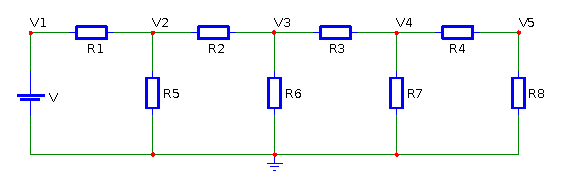
\includegraphics[width=12cm,angle=0]{./cap_linsis/pics/circuito_linear_8.eps}\label{circuitol8}
\end{center}
Complete a tabela abaixo representado a solução com 4 algarismos significativos:
\begin{center}
\begin{tabular}{|c|c|c|c|c|c|}
\hline
Caso & $V_1$ & $V_2$ & $V_3$ & $V_4$ & $V_5$\\
\hline
a & ~\hspace{40pt}~& ~\hspace{40pt}~& ~\hspace{40pt}~& ~\hspace{40pt}~& ~\hspace{40pt}~\\
\hline
b & & & & & \\
\hline
\end{tabular}
\end{center}
Então, refaça este problema reduzindo o sistema para apenas 4 incógnitas ($V_2$, $V_3$, $V_4$ e $V_5$).
\end{exer}
\begin{resp}
a)$V_5=98.44V$ b) $V_5=103.4V$
O problema com cinco incógnitas pode ser escrito na forma matricial conforme a seguir:
\begin{equation}\left[\begin{array}{ccccc}
1&0&0&0&0\\[.5cm]
\frac{1}{R_1}&-\left(\frac{1}{R_1}+\frac{1}{R_2}+\frac{1}{R_5}\right)&\frac{1}{R_2}&0&0\\[.5cm]
0&\frac{1}{R_2}&-\left(\frac{1}{R_2}+\frac{1}{R_3}+\frac{1}{R_6}\right)&\frac{1}{R_3}&0\\[.5cm]
0&0&\frac{1}{R_3}&-\left(\frac{1}{R_3}+\frac{1}{R_4}+\frac{1}{R_7}\right)&\frac{1}{R_4}\\[.5cm]
0&0&0&\frac{1}{R_4}&-\left(\frac{1}{R_4}+\frac{1}{R_8}\right)
\end{array}
\right]
\left[\begin{array}{c}
V_1\\[.65cm]
V_2\\[.65cm]
V_3\\[.65cm]
v_4\\[.65cm]
V_5
\end{array}
\right]=
\left[\begin{array}{c}
V\\[.65cm]
0\\[.65cm]
0\\[.65cm]
0\\[.65cm]
0
\end{array}
\right] \end{equation}
Este problema pode ser implementado no \verb+Scilab+ (para o item a) com o seguinte código:
\begin{verbatim}
R1=2, R2=2, R3=2, R4=2, R5=100, R6=100, R7=100, R8=50, V=127
A=[1      0                  0                  0                 0;
   1/R1  -(1/R1+1/R2+1/R5)   1/R2               0                 0;
   0      1/R2              -(1/R2+1/R3+1/R6)   1/R3              0;
   0      0                  1/R3             -(1/R3+1/R4+1/R7)   1/R4;
   0      0                  0                  1/R4             -(1/R4+1/R8)]
v=[V; 0; 0; 0; 0]
y=A\v
\end{verbatim}
O problema com quatro incógnitas pode ser escrito na forma matricial conforme a seguir:
\begin{equation}\left[\begin{array}{cccc}
-\left(\frac{1}{R_1}+\frac{1}{R_2}+\frac{1}{R_5}\right)&\frac{1}{R_2}&0&0\\[.5cm]
\frac{1}{R_2}&-\left(\frac{1}{R_2}+\frac{1}{R_3}+\frac{1}{R_6}\right)&\frac{1}{R_3}&0\\[.5cm]
0&\frac{1}{R_3}&-\left(\frac{1}{R_3}+\frac{1}{R_4}+\frac{1}{R_7}\right)&\frac{1}{R_4}\\[.5cm]
0&0&\frac{1}{R_4}&-\left(\frac{1}{R_4}+\frac{1}{R_8}\right)
\end{array}
\right]
\left[\begin{array}{c}
V_2\\[.65cm]
V_3\\[.65cm]
v_4\\[.65cm]
V_5
\end{array}
\right]=
\left[\begin{array}{c}
-\frac{V}{R1}\\[.65cm]
0\\[.65cm]
0\\[.65cm]
0
\end{array}
\right] \end{equation}
Cuja implementação pode ser feita conforme
\begin{verbatim}
A=[  -(1/R1+1/R2+1/R5)    1/R2               0                 0;
       1/R2              -(1/R2+1/R3+1/R6)   1/R3              0;
       0                  1/R3             -(1/R3+1/R4+1/R7)   1/R4;
       0                  0                  1/R4             -(1/R4+1/R8)]
v=[-V/R1; 0; 0; 0]
y=A\v
\end{verbatim}
\end{resp}
\begin{exer} Resolva o Problema~\ref{prob_circuito_resistores} pelos métodos de Jacobi e Gauss-Seidel.
\end{exer}
\begin{exer}(Interpolação) Resolva os seguintes problemas:
\begin{itemize}
\item[a)] Encontre o polinômio $P(x)=ax^2+bx+c$ que passa pelos pontos $(-1,-3)$, $(1,-1)$ e $(2,9)$.
\item[b)] Encontre os coeficientes $A$ e $B$ da função $f(x)=A\sin(x)+B\cos(x)$ tais que $f(1)=1.4$ e $f(2)=2.8$.
\item[c)] Encontre a função $g(x)=A_1\sin(x)+B_1\cos(x) + A_2\sin(2x)+B_2\cos(2x)$ tais que $f(1)=1$, $f(2)=2$, $f(3)=3$ e $f(4)=4$.
\end{itemize}
\end{exer}
\begin{resp}
Dica: $P(-1)=-3$, $P(1)=-1$ e $P(2)=9$ produzem três equações lineares para os coeficientes $a$, $b$ e $c$.
Resp: a) $P(x)=3x^2+x-5$, b) $A\approx 2.49$ e $B\approx -1.29$ c)$A_1\approx 1.2872058$, $A_2\approx - 4.3033034$, $B_1\approx 2.051533$ e $B_2\approx - 0.9046921$.
\end{resp}%%%% Extraído de ./cap_nlinsis/cap_nlinsis.tex
\chapter{Solução de sistemas de equações não lineares}\index{sistema de equações!não lineares}
\section{Método de  Newton para sistemas}\index{método de Newton!para sistemas}
\begin{exer} Faça o que se pede:
\begin{itemize}
\item[a)] Encontre o gradiente da função \begin{equation} f(x,y)=x^2y+\cos(xy)-4 \end{equation}
\item[b)] Encontre a matriz jacobiana associada à função
\begin{equation} F(x,y)=\left[\begin{array}{c}x\cos(x)+y\\ e^{-2x+y}\end{array} \right]. \end{equation}
\item[c)] Encontre a matriz jacobiana associada à função
\begin{equation}L(x)=\left[\begin{array}{c}
a_{11}x_1 + a_{12}x_2 +a_{13}x_3-y_1\\
a_{21}x_1 + a_{22}x_2 +a_{23}x_3-y_2\\
a_{31}x_1 + a_{32}x_2 +a_{33}x_3-y_3
\end{array}
 \right].\end{equation}
\end{itemize}
\end{exer}
\begin{resp}
$\nabla f = [2xy-y\sin(xy), x^2-x\sin(xy)]^T$
\begin{equation}J_F=\left[\begin{array}{cc}
\cos(x)-x\sin(x) & 1\\
-2e^{-2x+y} &e^{-2x+y}
\end{array}
\right]\end{equation}
\begin{equation} \left(J_L\right)_{ij}=a_{ij} \end{equation}
\end{resp}
\begin{exer} Encontre uma aproximação numérica para o seguinte problema não linear de três equações e três incógnitas:
\begin{eqnarray}
2x_1-x_2&=&\cos(x_1)\\
-x_1+2x_2-x_3&=&\cos(x_2)\\
-x_2+	x_3&=&\cos(x_3)
\end{eqnarray}
Partindo das seguintes aproximações iniciais:
\begin{itemize}
\item[a)] $x^{(0)}=[1,~1,~1]^T$
\item[b)] $x^{(0)}=[-0,5,~-2,~-3]^T$
\item[c)] $x^{(0)}=[-2,~-3,~-4]^T$
\item[d)] $x^{(0)}=[0,~0,~0]^T$
\end{itemize}
\end{exer}
\begin{resp}
  \construirResp
\end{resp}
\begin{exer}\label{prob_para_elipse}
 Encontre os pontos de intersecção entre a parábola $y=x^2+1$ e a elipse $x^2+y^2/4=1$ seguindo os seguintes passos:
\begin{itemize}
\item[a)] Faça um esboço das duas curvas e entenda o problema. Verifique que existem dois pontos de intersecção, um no primeiro quadrante e outro no segundo quadrante do plano $xy$.
\item[b)] A partir de seu esboço, encontre aproximações para $x$ e $y$ em cada ponto.
\item[c)] Escreva o problema na forma $F\left(\left[\begin{array}{c}x\\y\end{array}\right]\right)=\left[\begin{array}{c}0\\0\end{array}\right]$
\item[d)] Encontre a jacobiana $J_F$.
\item[e)] Construa a iteração do método de Newton.
\item[f)] Implemente no computador.
\item[g)] Resolva o sistema analiticamente e compare as respostas.
\end{itemize}
\end{exer}
\begin{resp}
As curvas possuem dois pontos de intersecção. A posição exata destes pontos de intersecção é dada por $\left(\sqrt{2\sqrt{3}-3},2\sqrt{3}-2\right)$ e $\left(-\sqrt{2\sqrt{3}-3},2\sqrt{3}-2\right)$. Use a solução exata para comparar com a solução aproximada obtida.
\end{resp}
\begin{exer} Encontre os pontos de intersecção entre a parábola $y=x^2$ e a curva $y=\cos(x)$ seguindo os seguintes passos:
\begin{itemize}
\item[a]) Faça um esboço das duas curvas, entenda o problema. Verifique que existem dois pontos de intersecção, um no primeiro quadrante e outro no segundo quadrante do plano $xy$.
\item[b]) A partir de seu esboço, encontre aproximações para $x$ e $y$ em cada ponto.
\item[c]) Escreva o problema na forma $F\left(\left[\begin{array}{c}x\\y\end{array}\right]\right)=\left[\begin{array}{c}0\\0\end{array}\right]$
\item[d]) Encontre a jacobiana $J_F$.
\item[e]) Construa a iteração do método de Newton.
\item[f]) Implemente no \ifisscilab\verb+Scilab+\fi\ifispython\verb+Python+\fi\ifisoctave\verb+Octave+\fi.
\item[g]) Transforme o sistema em um problema de uma única variável e compare com a resposta do Problema~\ref{1d:cosx2}.
%\item[h]) Refaça o item e, usando a função {\it derivative()} para aproximar a matriz jacobiana.
\end{itemize}
\end{exer}
\begin{resp}
 $\left(\pm 0.8241323, 0.6791941\right)$
\end{resp}
\begin{exer} Encontre uma aproximação com erro inferior a $10^{-5}$ em cada incógnita para a solução próxima da origem do sistema
\begin{eqnarray}
6x-2y+e^{z}&=&2\\
\sin(x)-y+z&=&0\\
\sin(x)+2y+3z&=&1
\end{eqnarray}
\end{exer}
\begin{resp}
$x\approx 0,259751, y\approx  0,302736, z\approx  0,045896$
\end{resp}
\begin{exer}(Entenda casos particulares)
\begin{itemize}
\item Considere a função $L(x)=Ax-b$, onde $A$ é uma matriz $n\times n$ inversível e $b$ um vetor coluna em $\mathbb{R}^n$. O que acontece quando aplicamos o método de Newton para encontrar as raízes de $L(x)$?
\item Mostre que o método de Newton-Raphson aplicado a uma função diferenciável do tipo $f:\mathbb{R}\to\mathbb{R}$ se reduz ao método de Newton estudado na primeira área.
\end{itemize}
\end{exer}
\begin{resp}
  \construirResp
\end{resp}
\begin{exer}\label{prob_bitang}Considere a função $f(x)=\frac{\sin(x)}{x+1}$, encontre a equação da reta que tangencia dois pontos da curva $y=f(x)$ próximos ao primeiro e segundo ponto de máximo no primeiro quadrante, respectivamente. Veja a Figura~\ref{pic:bitang}.
\end{exer}
\begin{resp}
  $y=mx+b$ com $m\approx - 0.0459710 $ e $b\approx 0.479237$
  Uma metodologia possível para resolver este problema é dada a seguir:
  Sejam $x_1$ e $x_2$ as abscissas dos dois pontos em que a reta tangencia a curva. A equação da reta bitangente assume a seguinte forma:
  \begin{equation} y=f(x_1) + m(x-x_1)  \end{equation}
  onde o coeficiente angular $m$ é dado por
  \begin{equation} m=\frac{f(x_2)-f(x_1)}{x_2-x_1} \end{equation}
  Da condição de tangência, temos que o coeficiente angular da reta, $m$, deve igual à derivada da função $f(x)$ nos dois pontos de tangência.
  \begin{equation} m=f'(x_1)=f'(x_2) \end{equation}
  E sabemos que:
  \begin{equation} f'(x)=\frac{\cos(x)}{1+x}-\frac{\sin(x)}{(1+x)^2}. \end{equation}
  Assim, podemos reescrever o problema como
  \begin{eqnarray}
\frac{\cos(x_1)}{1+x_1}-\frac{\sin(x_1)}{(1+x_1)^2}-\frac{\cos(x_2)}{1+x_2}+\frac{\sin(x_2)}{(1+x_2)^2}=0\\
\frac{\cos(x_1)}{1+x_1}-\frac{\sin(x_1)}{(1+x_1)^2}-\frac{f(x_2)-f(x_1)}{x_2-x_1}=0
\end{eqnarray}
Este é um sistema não linear de duas incógnitas.
Os valores iniciais para o método podem ser obtidos do gráfico buscando valores próximos aos dois primeiros pontos de máximos. Por exemplo: $x_1^{(0)}=1$ e $x_2^{(0)}=8$. Obtemos $x_1\approx 1,2464783$ e $x_2\approx 8,1782997$ e $m$ pode ser obtido através desses valores.
\end{resp}
\begin{exer}{(Estática)}\label{prob:dois_segmentos} Considere o sistema mecânico constituído de dois segmentos de mesmo comprimento $L$ presos entre si e a uma parede por articulações conforme a Figura~\ref{pic:dois_segmentos}.
O momento em cada articulação é proporcional à deflexão com constante de proporcionalidade $k$. Os segmentos são feitos de material homogêneo de peso $P$. A condição de equilíbrio pode ser expressa em termos dos ângulos $\theta_1$ e $\theta_2$ conforme:
\begin{eqnarray}
k\theta_1&=& \frac{3PL}{2}\cos\theta_1 + k\left(\theta_2-\theta_1\right)\\
k\left(\theta_2-\theta_1\right)&=& \frac{PL}{2}\cos\theta_2
\end{eqnarray}
Considere $P=100N$, $L=1m$ e calcule os ângulos $\theta_1$ e $\theta_2$ quando:
\begin{itemize}
\item[a)] $k=1000$ Nm/rad
\item[b)] $k=500$ Nm/rad
\item[c)] $k=100$ Nm/rad
\item[d)] $k=10$ Nm/rad
\end{itemize}
\noindent {\bf Obs:}Você deve escolher valores para iniciar o método. Como você interpretaria fisicamente a solução para produzir palpites iniciais satisfatórios? O que se altera entre o caso a e o caso d?
\end{exer}
\begin{resp}
$\left(0.1956550;0.2441719 \right)$, $\left(0.3694093;0.4590564\right) $, $\left( 0.9990712;1.1865168  \right)$ e $\left(1.4773606;1.5552232 \right)$
\end{resp}
\begin{exer}{(estática - problemas de três variáveis)} Considere, agora, o sistema mecânico semelhante ao do Problema~\ref{prob:dois_segmentos}, porém constituído de três segmentos de mesmo comprimento $L$ presos entre si e a uma parede por articulações.
O momento em cada articulação é proporcional à deflexão com constante de proporcionalidade $k$. Os segmentos são feitos de material homogêneo de peso $P$. A condição de equilíbrio pode ser expressa em termos dos ângulos $\theta_1$, $\theta_2$ e $\theta_3$ conforme:
\begin{eqnarray}
k\theta_1&=& \frac{5PL}{2}\cos\theta_1 + k\left(\theta_2-\theta_1\right)\\
k\left(\theta_2-\theta_1\right)&=& \frac{3PL}{2}\cos\theta_2+k\left(\theta_3-\theta_2\right)\\
k\left(\theta_3-\theta_2\right)&=& \frac{PL}{2}\cos\theta_3
\end{eqnarray}
Considere $P=10$N, $L=1$m e calcule os ângulos $\theta_1$, $\theta_2$ e $\theta_3$ quando:
\begin{itemize}
\item[a)] $k=1000$Nm/rad
\item[b)] $k=100$Nm/rad
\item[c)] $k=10$Nm/rad
\end{itemize}
\end{exer}
\begin{resp}
$\left(0.0449310; 0.0648872; 0.0698750  \right)$, $\left(0.3981385; 0.5658310; 0.6069019  \right)$, \\
$\left(1.1862966;1.4348545;1.480127  \right)$
\end{resp}
\begin{exer}  Considere o problema de encontrar os pontos de intersecção das curvas descritas por (ver Figura~\ref{pic:inter_curvas}):
\begin{eqnarray}
\frac{x^2}{8}+\frac{(y-1)^2}{5}&=&1\\~\\
\tan^{-1}(x)+x&=&y+y^3
\end{eqnarray}
 Com base no gráfico, encontre soluções aproximadas para o problema e use-as para iniciar o método de Newton-Raphson. Encontre as raízes com erro inferior a $10^{-5}$.
\end{exer}
\begin{resp}
$\left(-1,2085435, -1,0216674 \right)$ e $\left(2,7871115, 1,3807962\right)$
\ifisscilab
Exemplo de implementação:
\begin{verbatim}
function z=f(x,y)
    z=x^2/8+(y-1)^2/5-1
endfunction
function z=g(x,y)
    z=atan(x)+x-y-y^3
endfunction
contour([-3:.1:3],[-2:.1:4],f,[0 0])
contour([-3:.1:3],[-2:.1:4],g,[0 0])
function y=F(x)
    y(1)=f(x(1),x(2))
    y(2)=g(x(1),x(2))
endfunction
function y=JF(x)
    y(1,1)=x(1)/4
    y(1,2)=2*(x(2)-1)/5
    y(2,1)=1/(1+x(1)^2)+1
    y(2,2)=-1-3*x(2)^2
endfunction
//primeiro ponto
//x=[-1.2;-1.0]
//segundo ponto
//x=[2.8;1.4]
x=x-JF(x)\F(x)   // 4 vezes
\end{verbatim}
\fi
\end{resp}
\begin{exer} Considere o sistema de equações dado por
\begin{eqnarray}
\frac{(x-3)^2}{16}+\frac{(y-1)^2}{36}&=&1\\
\tanh(x)+x&=&2\sin y-0.01y^3
\end{eqnarray}
Usando procedimentos analíticos, determine uma região limitada do plano onde se encontram necessariamente todas as raízes do problema.
Encontre as raízes desse sistema com pelo menos quatro dígitos significativos corretos usando o método de Newton. Você deve construir o método de Newton indicando as funções envolvidas e calculando a matriz jacobiana analiticamente. Use que $\frac{d}{du}\tanh u = 1-\tanh^2u$, se precisar.
\end{exer}
\begin{resp}
 A primeira curva trata-se de uma elipse de centro $(3,1)$ e semi-eixos 4 e 6, portanto seus pontos estão contidos no retângulo $-1\leq x \leq 7$ e $-5\leq y \leq 7$.
As soluções são $\left( -0,5384844 , -1,7978634\right)$ e $\left(2,8441544, 6,9954443\right)$.
\ifisscilab
Uma possível implementação é
\begin{verbatim}
function z=f(x,y)
    z=(x-3)^2/16+(y-1)^2/36-1
endfunction
function z=g(x,y)
    z=atan(x)+x-sin(y)-0.01*y^3
endfunction
contour([-1:.1:7],[-5:.1:7],f,[0 0])
contour([-1:.1:7],[-5:.1:7],g,[0 0])
function y=F(x)
    y(1)=f(x(1),x(2))
    y(2)=g(x(1),x(2))
endfunction
function y=JF(x)
    y(1,1)=(x(1)-3)/8
    y(1,2)=(x(2)-1)/18
    y(2,1)=1/(1+x(1)^2)+1
    y(2,2)=-cos(x(2))-0.03*x(2)^2
endfunction 
//primeiro ponto
//x=[-.5;-2.0]
//segundo ponto
//x=[3;7]
x=x-JF(x)\F(x)   // 4 vezes
\end{verbatim}
\fi
\end{resp}
\begin{exer}(Otimização)\label{nlinsis:usinas} Uma indústria consome energia elétrica de três usinas fornecedoras. O custo de fornecimento em reais por hora como função da potência consumida em kW é dada pelas seguintes funções
\begin{eqnarray}
C_1(x)&=&10+.3x+10^{-4}x^2+3.4\cdot 10^{-9}x^4\\
C_2(x)&=&50+.25x+2\cdot 10^{-4}x^2+4.3\cdot 10^{-7}x^3\\
C_3(x)&=&500+.19x+5\cdot 10^{-4}x^2+1.1\cdot 10^{-7}x^4
\end{eqnarray}
Calcule a distribuição de consumo que produz custo mínimo quando a potência total consumida é $1500kW$. Dica: Denote por $x_1$, $x_2$ e $x_3$ as potências consumidas das usinas 1, 2 e 3, respectivamente.  O custo total será dado por $C(x_1,x_2,x_3)=C_1(x_1)+C_2(x_2)+C_3(x_3)$ enquanto o consumo total é $x_1+x_2+x_3=1500$. Isto é, queremos minimizar a função custo total dada por:
\begin{equation} C(x_1,x_2,x_3)=C_1(x_1)+C_2(x_2)+C_3(x_3) \end{equation}
restrita à condição
\begin{equation} G(x_1,x_2,x_3)=x_1+x_2+x_3-1500=0. \end{equation}
Pelos multiplicadores de Lagrange, temos que resolver o sistema dado por:
\begin{eqnarray}
\nabla C(x_1,x_2,x_3) &=& \lambda \nabla G(x_1,x_2,x_3)\\
G(x_1,x_2,x_3)&=&0
\end{eqnarray}
\end{exer}
\begin{resp}
 $(x_1,x_2,x_3)\approx (453,62,~ 901,94,~ 144,43)$
\end{resp}
\begin{exer} \label{nlinsis:prob_ajuste_eax} Encontre a função do tipo $f(x)=Ab^{x}$ que melhor aproxima os pontos $(0,~3,1)$, $(1,~4,4)$ e $(2,~6,7)$ pelo critério dos mínimos quadrados. Dica: Você deve encontrar os valores de $A$ e $b$ que minimizam o resíduo dado por
\begin{equation} R=\left[3,1-f(0)\right]^2+\left[4,4-f(1)\right]^2+\left[6,7-f(2)\right]^2. \end{equation}
{\bf Dica:} Para construir aproximações para resposta e iniciar o método, considere a função $f(x)=Ab^x$ que passa pelo primeiro e terceiro ponto.
\end{exer}
\begin{resp}
Inicialização do método: $A^{(0)}= 3,1$ e $b^{(0)}= \sqrt{\frac{6,7}{3,1}}$
$A\approx  3.0297384 $ e $b\approx 1.4835346$.
\end{resp}
\begin{exer}Encontre o valor máximo da função \begin{equation} f(x,y)=-x^4-y^6+3xy^3-x \end{equation} na região $(x,y)\in [-2,0]\times [-2,0]$
 seguindo os seguintes passos:
\begin{itemize}
  \item[a)] Defina a função $z=f(x,y)=-x^4-y^6+3xy^3-x$ e trace o gráfico de contorno na região.
  \item[b)] Com base no gráfico, encontre valores aproximados para as coordenadas $xy$ do ponto de máximo.
  \item[c)] Sabendo que o ponto de máximo acontece quando o gradiente é nulo, escreva o problema como um sistema de duas equações não lineares e duas incógnitas.
  \item[d)] Implemente o método de Newton.
\end{itemize}
\end{exer}
 \begin{resp}
 $f(-1,1579702, -1,2020694)\approx 2.376985$
\ifisscilab
Um exemplo de implementação no Scilab é:
\begin{verbatim}
deff('z=f(x,y)','z=-x^4-y^6+3*x*y^3-x')
contour([-2:.01:0],[-2:.01:0],f,[ 0:.2: 3])
deff('z=F(x)','z=[-4*x(1)^3+3*x(2)^3-1;-6*x(2)^5+9*x(1)*x(2)^2]')
deff('z=JF(x)','z=[-12*x(1)^2,9*x(2)^2;9*x(2)^2,-30*x(2)^4+18*x(1)*x(2)]')
x=[-1.2;-1.2]
x=x-JF(x)\F(x)
x=x-JF(x)\F(x)
x=x-JF(x)\F(x)
x=x-JF(x)\F(x)
mprintf('f(%f,%f)=%f',x(1),x(2),f(x(1),x(2)))
\end{verbatim}
\fi
\end{resp}
\begin{exer}A função $f(x,y,z)=\sin(x)+\sin(2y)+\sin(3z)$ possui um máximo quando $x=\pi/2$, $y=\pi/4$ e $z=\pi/6$. Calcule numericamente este ponto.
\end{exer}
\begin{resp}
  \construirResp
\end{resp}
\begin{exer}\label{prob_sis3} Encontre as raízes do problema
  \begin{eqnarray}
    3x-\cos(yz+z)-1/2&=&0\\
    4x^2-25y^2+0.4y+2&=&0\\
    e^{-xy}+2x-5z&=&10
  \end{eqnarray}
  no cubo $|x|<2, |y|<2, |z|<2.$
  Dica: Reduza a um problema de duas incógnitas e use recursos gráficos para aproximar as raízes na região.
\end{exer}
\begin{resp}
  $x\approx 0,2982646, y\approx -0,2990796, z\approx- 1,6620333$  e $x\approx -0,0691328, y\approx 0,2923039, z\approx -0,8235705$.
\end{resp}
\begin{exer}  Considere o seguinte sistema de equações não lineares:
\begin{eqnarray}
x_1-x_2&=&0\nonumber\\
-x_{j-1}+5(x_j+x_j^3)-x_{j+1}&=&10\exp(-j/3),~~ 2\leq j \leq 10\nonumber\\
x_{11}&=&1
\end{eqnarray}
\begin{itemize}
\item [a)] Escreva este sistema na forma $F(x)=0$ onde $x=\left[\begin{array}{c} x_1\\ x_2\\ \vdots \\ x_{11}\end{array}\right]$ e calcule analiticamente a matriz jacobiana $\frac{\partial (F_1,\ldots, F_{11})}{\partial (x_1,\ldots x_{11})}$. Dica: Use a regularidade nas expressões para abreviar a notação.
\item [b)] Construa a iteração para encontrar a única solução deste problema pelo método de Newton e, usando esse método, encontre uma solução aproximada com erro absoluto inferior a $10^{-4}$.
\end{itemize}
\end{exer}
\begin{resp}
\begin{equation}F\left(x\right)=\left[
\begin{array}{c}
x_1-x_2\\[.2cm]
-x_{1}+5(x_2+x_2^3)-x_{3}-10\exp(-2/3)\\[.2cm]
-x_{2}+5(x_3+x_3^3)-x_{4}-10\exp(-3/3)\\[.2cm]
-x_{3}+5(x_4+x_4^3)-x_{5}-10\exp(-4/3)\\[.2cm]
\vdots\\
-x_{9}+5(x_{10}+x_{10}^3)-x_{11}-10\exp(-10/3)\\[.2cm]
x_{11}-1
\end{array}\right] \end{equation}
\begin{equation}J_F(x)=\left[
\begin{array}{ccccccc}
1& -1 &0 &0 &0&\ldots & 0\\[.2cm]
-1&5(1+3x_2^2)& -1&0&0&\ldots & 0\\[.2cm]
0&-1&5(1+3x_3^2)& -1&0&\ldots & 0\\[.2cm]
0&0&-1&5(1+3x_4^2)& -1&\ldots & 0\\[.2cm]
\vdots &\vdots &\vdots &\vdots &&\ddots&\vdots\\[.2cm]
0&0&0&0&0&\cdots&1
\end{array}
\right]
\end{equation}
\ifisscilab
Exemplo de implementação no Scilab:
\begin{verbatim}
function y=F(x)
    y(1)=x(1)-x(2)
    for j=2:10
        y(j)=-x(j-1)+5*(x(j)+x(j)^3)-x(j+1)-10*exp(-j/3)
    end
    y(11)=x(11)-1
endfunction
function y=JF(x)
    y=zeros(11,11)
    y(1,1)=1
    y(1,2)=-1
    for j=2:10
        y(j,j-1)=-1
        y(j,j)=5*(1+3*x(j)^2)
        y(j,j+1)=-1
    end
    y(11,11)=1
endfunction
\end{verbatim}
\fi
Resposta final: 0,80447, 0,80447, 0,68686, 0,57124, 0,46535,
0,37061, 0,28883, 0,22433, 0,19443, 0,28667,  1
\end{resp}
\begin{exer} Considere a função
\begin{equation} f(x,y)=\frac{e^{-(x-1)^2-(y-2)^2}}{1+x^2+y^2} \end{equation}
\begin{itemize}
\item[a)] Encontre o valor máximo desta função.
\item[b)] Usando multiplicadores de Lagrange, encontre o valor máximo desta função restrito à condição \begin{equation} (x-1)^2+(y-2)^2=1. \end{equation}
\item[c)] Parametrize a circunferência para transformar o problema de máximo com restrição em um problema de uma única variável. Resolva usando as técnicas de equações lineares de uma variável.
\end{itemize}
\end{exer}
\begin{resp}
$f(0,8108792, 1,6217584)\approx 0,1950369$ e $f(0,5527864, 1,1055728 )\approx 0,1455298 $
\end{resp}
\stepcounter{section}%%%% Extraído de ./cap_interp/cap_interp.tex
\chapter{Interpolação}\index{aproximação!de funções}\label{cap:interp}
\section{Interpolação polinomial}\index{interpolação!polinomial}
\begin{exer}\label{exer:interp1}
Encontre o polinômio interpolador para o conjunto de pontos $\{(-2, -47)$, $(0, -3)$, $(1, 4)$, $(2, 41)\}$. Então, faça um gráfico com os pontos e o polinômio interpolador encontrado.
\end{exer}
\begin{resp}
  $p(x) = -3 + 2x + 5x^3$.
\end{resp}
\begin{exer}
  Encontre o polinômio interpolador para o conjunto de pontos $\{(-1, 1,25)$, $(0,5, 0,5)$, $(1, 1,25)$, $(1,25, 1,8125)\}$.
\end{exer}
\begin{resp}
  $p(x) = 0,25 + x^2$.
\end{resp}
\stepcounter{section}\stepcounter{section}\section{Aproximação de funções reais por polinômios interpoladores}\index{aproximação!de funções!por polinômios}
\begin{exer}
  Use as mesmas técnicas usadas o resultado do Exemplo~\ref{exemp_simpson} para obter uma aproximação do valor de:
  \begin{equation}
    \int_0^1 f(x)dx
  \end{equation}
através do polinômio interpolador que coincide com $f(x)$ nos pontos $x=0$ e $x=1$.
\end{exer}
\begin{resp}
  $\int_0^1 P(x)dx =\frac{f(0)+f(1)}{2}$, $\frac{1}{12}\max_{x\in[0,1]}|f''(x)|$
\end{resp}
\stepcounter{section}\section{Interpolação cúbica segmentada - spline}\index{interpolação!cúbica segmentada}\index{spline}
% \begin{exer} Considere o problema de encontrar as parâmetro $A$, $B$ e $\lambda$ tais que a função $f(x)=A+B e^{\lambda x}$ passa por três pontos dados.
% \begin{itemize}
% \item[a)] Verifique que se $A=1$, $B=2$ e $\lambda=-\ln(2)$ então $f(0)=3$, $f(1)=2$ e $f(2)=1.5$
% \item[b)] Encontre os valores de $A$, $B$ e $\lambda$ tais que $f(0)=3.1$, $f(1)=1.9$ e $f(2)=1.6$
% \item[c)] Encontre os valores de $A$, $B$ e $\lambda$ tais que $f(0)=2.9$, $f(1)=2.1$ e $f(2)=1.6$
% \item[d)] Compare os parâmetros para cada um dos três casos. Discuta a viabilidade do problema de ajustar curvas desse tipo a um conjunto de dados com erro experimental.
%
% {\bf Dica:} Calcule  número de condicionamento da matriz jacobiana associada ao problema no caso a.
% \end{itemize}
% \end{exer}
% \begin{resp}
% $1.5,1.6 ,- 1.3862944$ e $0.7666667 , 2.1333333 ,- 0.4700036$
% \end{resp}
% \begin{exer} Considere o problema de encontrar as parâmetros $A$, $B$, $\lambda_1$ e $\lambda_2$ tais que a função $f(x)=Ae^{\lambda_1 x}+B e^{\lambda_2 x}$ passa por quatro pontos dados.
% \begin{itemize}
% \item[a)] Verifique que função se $A=10$, $B=20$, $\lambda_1=\ln(2)$ e $\lambda_2=\ln(3)$ então $f(-1)=35/3$, $f(0)=30$, $f(1)=80$, $f(2)=220$
% \item[b)] Imagine que você desconheça os valores de $A$, $B$, $\lambda_1$ e $\lambda_2$ no item acima e deseja encontrá-los com base nos valores da função nos quatro pontos dados pelo método de Newton-Raphson com quatro incóginta. Descreva a função jacobiana envolvida e calcule o número de condicionamento quando as incógnitas são dadas conforme o item a.
% \item[c)] Implemente o método de Newton-Raphson a partir das condições iniciais dadas pelos valores numéricos aproximados de $A=10$, $B=20$, $\lambda_1=\ln(2)$ e $\lambda_2=\ln(3)$ (ou seja, a solução exata acrescida de erros de arredondamento). Discuta.
% \end{itemize}
% \end{exer}
% \begin{resp}
% O número de condicionamento é $k_2 \approx 10^9$.
% \end{resp}%%%% Extraído de ./cap_ajuste/cap_ajuste.tex
\chapter{Ajuste de curvas}\index{aproximação!de funções}\index{ajuste!por mínimos quadrados}
\section{Ajuste de uma reta}\index{ajuste!de uma reta}
\begin{exer}
  Sejam dados o conjunto de pontos $\{(0,23, -0,54)$, $(-0,30, -0,54)$, $(0,04, -0,57)\}$. Encontre a função $f(x) = a_1 + a_2x$ que melhor se ajusta no sentido de mínimos quadrados aos pontos dados. Faça, então, um gráfico com os pontos e o esboço da função ajustada.
\end{exer}
\begin{resp}
    $f(x) = -0,55 -0,01x$.
\end{resp}
\begin{exer}
  Seja dado o conjunto de pontos $\{(-0,35, 0,2)$, $(0,15, -0,5)$, $(0,23, 0,54)$, $(0,35, 0,7)\}$. Encontre a função $f(x) = a_1 + a_2x$ que melhor se ajusta no sentido de mínimos quadrados aos pontos dados. Faça, então, um gráfico com os pontos e o esboço da função ajustada.
\end{exer}
\begin{resp}
    $f(x) = 0,19 - 0,47x$.
\end{resp}
\begin{exer}
  Seja dado o conjunto de pontos $\{(-1,94, 1,02)$, $(-1,44, 0,59)$, $(0,93, -0,28)$, $(1,39, -1,04)\}$. Encontre a função $f(x) = a_1 + a_2x$ que melhor se ajusta no sentido de mínimos quadrados aos pontos dados. Então, responda cada item:
  \begin{enumerate}[a)]
  \item Encontre o valor de $f(1)$.
  \item Encontre o valor de $f(0,93)$.
  \item Encontre o valor de $|f(0,93) - (- 0,28)|$.
  \item Encontre o valor do resíduo $R = \sum_{j=1}^N (f(x_j)-y_j)^2$.
  \end{enumerate}
Forneça os valores calculados com $7$ dígitos significativo por arredondamento.
\end{exer}
\begin{resp}
    a)~$-0,6025387$; b)~$-0,5651848$; c)~$0,2851848$; d)~$0,1488041$.
\end{resp}
\section{Ajuste linear geral}\index{ajuste!linear}
\begin{exer}
  Encontre o polinômio $p(x) = a_1 + a_2x + a_3x^2$ que melhor se ajusta no sentido de mínimos quadrados aos pontos:
  \begin{center}
    \begin{tabular}{l|cccc}
      $i$ & $1$ & $2$ & $3$ & $4$ \\\hline
      $x_i$ & $-1,50$ & $-0,50$ & $1,25$ & $1,50$\\
      $y_i$ & $1,15$ & $-0,37$ & $0,17$ & $0,94$
  \end{tabular}
    \end{center}
\end{exer}
\begin{resp}
    $a_1 = -0,67112$, $a_2 = -0,12123$, $a_3 = 0,73907$.
\end{resp}
\begin{exer}Encontrar a parábola $y=ax^2+bx+c$ que melhor aproxima o seguinte conjunto de dados:
  \begin{center}
    \begin{tabular}{l|ccccc}
      $i$ & $1$ & $2$ & $3$ & $4$ & $5$ \\\hline
      $x_i$ & $0,01$ & $1,02$ & $2,04$ & $2,95$ & $3,55$\\
      $y_i$ & $1,99$ & $4,55$ & $7,20$ & $9,51$ & $10,82$
    \end{tabular}
  \end{center}
\end{exer}
\begin{resp}
    $y=-0,0407898x^2+ 2,6613293x+ 1,9364598$.
\end{resp}
\begin{exer} Dado o seguinte conjunto de dados
  \begin{center}
    \begin{tabular}{l|ccccccccccc}
      $x_i$ & $0,0$ & $0,1$ & $0,2$ & $0,3$ & $0,4$ & $0,5$ & $0,6$ & $0,7$ & $0,8$ & $0,9$ & $1,0$\\\hline
      $y_i$ & $31$ & $35$ & $37$ & $33$ & $28$ & $20$ & $16$ & $15$ & $18$ & $23$ & $31$
    \end{tabular}
  \end{center}
\begin{enumerate}[a)]
\item Encontre a função do tipo $f(x)=a+b\sin(2\pi x)+c\cos(2\pi x)$ que melhor aproxima os valores dados.
\item Encontre a função do tipo $f(x)=a+bx+cx^2+dx^3$ que melhor aproxima os valores dados.
\end{enumerate}
\end{exer}
\begin{resp}
    a) $a=25,638625$, $b=9,8591874$, $c=4,9751219$; b)$a=31,475524$, $b=65,691531$, $c=-272,84382$, $d=208,23621$.
\end{resp}
% \begin{exer}Encontre a partir de primeiros princípios a função do tipo $f(x)=bx+a$ que melhor aproxima os pontos:
%   \begin{equation}
%     (0,-0,1), (1,~2), (2,~3,7) ~ \text{e} ~(3,~7).
%   \end{equation}
% \end{exer}
% \begin{resp}
% \begin{eqnarray}
% E_q&=&[f(0)+0,1]^2+[f(1)-2]^2+[f(2)-3,7]^2+[f(3)-7]^2\\
% &=&[a+0,1]^2+[a+b-2]^2+[a+2b-3,7]^2+[a+3b-7]^2
% \end{eqnarray}
% Devemos encontrar os parâmetros $a$ $b$ que minimizam o erro, por isso, calculamos as derivadas parciais:
% \begin{eqnarray}
% \frac{\partial E_q}{\partial a}&=&2[a+0,1]+2[a+b-2]+2[a+2b-3,7]+2[a+3b-7]\\
% \frac{\partial E_q}{\partial b}&=&2[a+b-2]+4[a+2b-3,7]+6[a+3b-7]
% \end{eqnarray}
% O erro mínimo acontece quando as derivadas são nulas, ou seja:
% \begin{eqnarray}
% 8a+12b&=&25,2\\
% 12a+28b&=&60,8
% \end{eqnarray}
% Cuja solução é dada por $a=-0,3$ e $b=2,3$.
% Portanto a função que procuramos é $f(x)=-0,3 +2,3x$.
% \end{resp}
% \begin{exer} Encontre a função do tipo $f(x)=ax$ que melhor se aproxima dos seguintes pontos:
%   \begin{equation}
%     (0, -0,1), (1, 2), (2, 3,7) ~ \text{e} ~(3, 7).
%   \end{equation}
% \end{exer}
% \begin{resp}
% Defina \begin{equation} E_q=[f(x_1)-y_1]^2+[f(x_2)-y_2]^2+[f(x_3)-y_3]^2+[f(x_4)-y_4]^2 \end{equation}
% temos que
% \begin{eqnarray}
% E_q&=&[f(0)+0,1]^2+[f(1)-2]^2+[f(2)-3,7]^2+[f(3)-7]^2\\
% &=&[0,1]^2+[a-2]^2+[2a-3,7]^2+[3a-7]^2
% \end{eqnarray}
% Devemos encontrar o parâmetro $a$ que minimiza o erro, portanto, calculamos:
% \begin{eqnarray}
% \frac{\partial E_q}{\partial a}&=&2[a-2]+4[2a-3,7]+6[3a-7]=28a-60,8
% \end{eqnarray}
% Portanto o valor de $a$ que minimiza o erro é $a=\frac{60,8}{28}$.
% \ifisscilab
% \begin{verbatim}
% x=[0 1 2 3]'
% y=[-.1 2 3.7 7]'
% plot2d(x,y,style=-4)
% \end{verbatim}
% \fi
% \end{resp}
\stepcounter{section}%%%% Extraído de ./cap_derivacao/cap_derivacao.tex
\chapter{Derivação numérica}\index{derivação}
\section{Diferenças finitas}\index{diferenças finitas}
\begin{exer}
Use os esquemas numéricos de diferença finita regressiva de ordem 1, diferença finita progressiva de ordem 1 e diferença finita central de ordem 2 para aproximar as seguintes derivadas:
\begin{itemize}
\item[a)] $f'(x)$ onde $f(x)=\sen(x)$ e $x=2$.
\item[b)] $f'(x)$ onde $f(x)=e^{-x}$ e $x=1$.
\end{itemize}
Use $h=10^{-2}$ e $h=10^{-3}$ e compare com os valores obtidos através da avaliação numérica das derivadas exatas.
\end{exer}
\begin{resp}
  \begin{itemize}
\item[a)] $f'(x)$ onde $f(x)=\sen(x)$ e $x=2$ para $h=10^{-2}$ e $h=10^{-3}$, respectivamente.
\subitem Progressiva ordem 1: $-0,42069$ e $-0,41660$.
\subitem Regressiva ordem 1: $-0,41159$ e $-0,41569$.
\subitem Central ordem 2: $-0,41614$ e $-0,41615$.
\subitem Exata: $\cos(2)=-0,41615$
\item[b)] $f'(x)$ onde $f(x)=e^{-x}$ e $x=1$ para $h=10^{-2}$ e $h=10^{-3}$, respectivamente.
\subitem Progressiva ordem 1: $-0,36605$ e $-0,36788$.
\subitem Regressiva ordem 1: $-0,36972$ e $-0,36806$.
\subitem Central ordem 2: $-0,36789$ e $-0,36788$.
\subitem Exata: $-e^{-1}=-0,36788$
  \end{itemize}
 \end{resp}
\begin{exer}\label{ex1} Expanda a função suave $f(x)$ em um polinômio de Taylor adequado para obter as seguintes aproximações:
\begin{itemize}
\item[a)] $f'(x)=\frac{f(x+h)-f(x)}{h}+\mathcal{O}(h)$
\item[b)] $f'(x)=\frac{f(x)-f(x-h)}{h}+\mathcal{O}(h)$
\item[c)] $f'(x)=\frac{f(x+h)-f(x-h)}{2h}+\mathcal{O}(h^2)$
\end{itemize}
\end{exer}%resposta no texto
\begin{exer} Use a expansão da função $f(x)$ em torno de $x=0$ em polinômios de Taylor para encontrar os coeficientes $a_1$, $a_2$ e $a_3$ tais que
\begin{itemize}
\item[a)] $f'(0)=a_1f(0)+a_2f(h)+a_3f(2h) + \mathcal{O}(h^2)$
\item[b)] $f'(0)=a_1f(0)+a_2f(-h)+a_3f(-2h) + \mathcal{O}(h^2)$
\item[c)] $f'(0)=a_1f(-h_1)+a_2f(0)+a_3f(h_2) + \mathcal{O}(h^2),~~|h_1|, |h_2|=\mathcal{O}(h)$
\end{itemize}
\end{exer}
\begin{resp}
%  
\begin{itemize}
\item[a)] $f'(0)=\frac{-3f(0)+4f(h)-f(2h)}{2h} + \mathcal{O}(h^2)$
\item[b)] $f'(0)=\frac{3f(0)-4f(-h)+f(-2h)}{2h} + \mathcal{O}(h^2)$
\item[c)] $f'(0)=\frac{1}{h_1+h_2}l\left[-\frac{h_2}{h_1}f(-h_1) +\left(\frac{h_2}{h_1}-\frac{h_1}{h_2}\right)f(0)+ \frac{h_1}{h_2}f(h_2)\right]$
\end{itemize}    
%  
\end{resp}
\begin{exer} As tensões  na entrada, $v_i$, e saída, $v_o$, de um amplificador foram medidas em regime estacionário conforme tabela abaixo.
  \begin{center}
    \begin{tabular}{|c|c|c|c|c|c|c|c|c|c|c|}\hline
    0,0 &   0,50  &   1,00   &   1,50  &   2,00 &     2,50   &  3,00  &    3,50  &   4,00  &    4,50  &   5,00\\ \hline
    0,0  &  1,05  &  1,83  &  2,69  &  3,83 &   4,56 &   5,49 &   6,56  &  6,11 &   7,06  &  8,29\\ \hline 
    \end{tabular}
  \end{center}
onde  a primeira linha é a tensão de entrada em volts e a segunda linha é tensão de saída em volts.
Sabendo que o ganho é definido como \begin{equation} \frac{\partial v_o}{\partial v_i}. \end{equation} Calcule o ganho quando $v_i=1$ e $v_i=4.5$ usando as seguintes técnicas:
\begin{itemize}
\item[a)] Derivada primeira numérica de primeira ordem usando o próprio ponto e o próximo.
\item[b)] Derivada primeira numérica de primeira ordem usando o próprio ponto e o anterior.
\item[c)] Derivada primeira numérica de segunda ordem usando o ponto anterior e o próximo.
\item[d)] Derivada primeira analítica da função do tipo $v_0=a_1 v_i + a_3 v_i^3$ que melhor se ajusta aos pontos pelo critério dos mínimos quadrados.
\end{itemize}
\begin{center}
\begin{tabular}{|c|c|c|c|c|}\hline
 Caso &  a  &   b &   c   &   d \\ \hline
 $v_i=1$ &    & ~\hspace{50pt}~  &   & ~\hspace{50pt}~ \\ \hline
$v_i=4.5$ &~\hspace{50pt}~    &   &  ~\hspace{50pt}~   &\\ \hline
\end{tabular}
\end{center}
% \ifisscilab
% Dica:
% \begin{verbatim}
% y=[0 1.05 1.83 2.69 3.83 4.56 5.49 6.56 6.11 7.06 8.29]
% \end{verbatim}
% \fi
\end{exer}
\begin{resp}
\begin{equation}\begin{array}{|c|c|c|c|c|}\hline
 Caso &  a  &   b &   c   &   d \\ \hline
 v_i=1 & 1.72   & 1.56  &  1.64 & 1.86 \\ \hline
v_i=4.5 &2.46    & 1.90  &  2.18  &1.14  \\ \hline
\multicolumn{5}{c}{}
\end{array}
\end{equation}    
\end{resp}
\begin{exer}Estude o comportamento da derivada de $f(x)=e^{-x^2}$ no ponto $x=1,5$ quando $h$ fica pequeno.
\end{exer}
\begin{resp}
Segue a tabela com os valores da derivada para vários valores de $h$.
\begin{equation}
\begin{array}{|c|c|c|c|c|c|c|}\hline
h&10^{-2}&10^{-4}&10^{-6}&10^{-7}&10^{-8}&10^{-9}\\\hline
D_{+,h}f(1,5)& - 0,3125246&- 0,3161608 &- 0,3161973&- 0,3161976&- 0,3161977&- 0,3161977 \\\hline
\multicolumn{7}{c}{}
\end{array}  
\end{equation}  
\begin{equation}
\begin{array}{|c|c|c|c|c|c|c|}\hline
h&10^{-10}&10^{-11}&10^{-12}&10^{-13}&10^{-14}&10^{-15}\\\hline
D_{+,h}f(1,5)&- 0,3161976&- 0,3161971&- 0,3162332&- 0,3158585&- 0,3178013&- 0,3747003\\\hline
\multicolumn{7}{c}{}
\end{array}
\end{equation}
Observe que o valor exato é $-0,3161977$ e o $h$ ótimo é algo entre $10^{-8}$ e $10^{-9}$.        
\end{resp}
\section{Diferença finita para derivada segunda}\index{fórmula de diferenças finitas!central}
\begin{exer} Use a expansão da função $f(x)$ em torno de $x=0$ em polinômios de Taylor para encontrar os coeficientes $a_1$, $a_2$ e $a_3$ tais que
\begin{itemize}
\item[a)] $f''(0)=a_1f(0)+a_2f(h)+a_3f(2h) + \mathcal{O}(h)$
\item[b)] $f''(0)=a_1f(0)+a_2f(-h)+a_3f(-2h) + \mathcal{O}(h)$
\end{itemize}
\end{exer}
\begin{resp}
\begin{itemize}
\item[a)] $f''(0)=\frac{f(0)-2f(h)+f(2h)}{h^2}+\mathcal{O}(h)$
\item[b)] $f''(0)=\frac{f(0)-2f(-h)+f(-2h)}{h^2}+\mathcal{O}(h)$
\end{itemize}    
\end{resp}
\stepcounter{section}\section{Fórmulas de diferenças finitas}
\begin{exer}
Seja $\{x_0, x_1, x_2\}=\{0, h, 2h\}$ e $x^*=x_0=0$, obtenha uma regra unilateral de diferenciação para aproximar $f'(x_0)$.
\end{exer}%sem resposta
\begin{exer}
Seja $\{x_0, x_1, x_2\}=\{-h, 0, h\}$ e $x^*=x_1=0$, obtenha uma regra de diferenciação para aproximar $f''(x^*)$.
\end{exer}
\begin{resp}
 $f''(x^*)=\frac{f(x_0)-2f(x_1)+f(x_2)}{h^2}$ 
\end{resp}
\begin{exer}
Seja $\{x_0, x_1, \ldots, x_4\}=\{-2h, -h, 0, h, 2h\}$ e $x^*=0$, obtenha uma regra de diferenciação para aproximar $f'(x^*)$.
\end{exer}%sem resposta
\begin{exer}
Seja $[x_0,x_1,\ldots ,x_4]=[-2h,-h,0,h,2h]$ e $x^*=0$, obtenha uma regra de diferenciação para aproximar $f''(x^*)$.
\end{exer}%sem resposta
\begin{exer}
Seja $[x_0,x_1,\ldots ,x_4]=[0,h,3h,6h,10h]$ e $x^*=0$, obtenha uma regra de diferenciação para aproximar $f'(x^*)$.
\end{exer}%sem resposta
\stepcounter{section}\stepcounter{section}%%%% Extraído de ./cap_integracao/cap_integracao.tex
\chapter{Integração numérica}\index{integração} \label{cap:integracao}
\stepcounter{section}\stepcounter{section}% \section{Regras de Newton-Cotes}\index{integração numérica!regras de Newton-Cotes}
\begin{exer}Calcule numericamente as seguintes integrais:
  \begin{eqnarray}
    \text{a)}~\int_0^1e^{-x}\,dx & \text{b)}~\int_0^1x^2\,dx\\
    \text{c)}~\int_0^1x^3\,dx & \text{d)}~\int_0^1xe^{-x^2}\,dx\\
    \text{e)}~\int_0^1\frac{1}{x^2+1}\,dx &\text{e)}~\int_0^1\frac{x}{x^2+1}\;dx
  \end{eqnarray}
usando os métodos simples do ponto médio, Trapézio e Simpson. Calcule, também, o valor analítico destas integrais e o erro nas aproximações dadas pelas quadraturas numéricas.
\end{exer}
% \begin{resp}
%
%  \begin{center}
% \begin{tabular}{|c|c|c|c|c|}
% \hline
%   & exato & Ponto médio & Trapézio & Simpson \\
% \hline
%  & & & &\\[-.3cm]
% $\int_0^1e^{-x}dx$ &$1-e^{-1}\approx 0.6321206$& $ e^{-1/2}\approx 0.6065307$&$\frac{1+e^{-1}}{2}\approx 0.6839397$ &$\frac{1+4e^{-1/2}+e^{-1}}{6}\approx 0.6323337$\\[.2cm]
% \hline
%  & & & &\\[-.3cm]
% $\int_0^1x^2dx $ & $1/3\approx 0.3333333$& 0.25 & 0.5 & 0.3333333\\[.2cm]
% \hline
%  & & & &\\[-.3cm]
% $\int_0^1x^3dx $ & $1/4=0.25$ & 0.125 & 0.5 & 0.25\\[.2cm]
% \hline
%  & & & &\\[-.3cm]
% $\int_0^1xe^{-x^2}dx$  &$\frac{1}{2}\left(1-e^{-1}\right)\approx 0.3160603$ & 0.3894004  &  0.1839397 &   0.3209135  \\[.2cm]
% \hline
%  & & & &\\[-.3cm]
% $\int_0^1\frac{1}{x^2+1}dx$  & $\tan^{-1}(1)\approx 0.7853982$ &  0.8  &  0.75 &   0.7833333
%  \\[.2cm]
% \hline
%  & & & &\\[-.3cm]
% $\int_0^1\frac{x}{x^2+1}dx$  &$\frac{1}{2}\ln(2)\approx  0.3465736  $ & 0.4 & 0.25 & 0.35\\[.2cm]
% \hline
%  & & & &\\[-.3cm]
% $\int_0^1\frac{1}{x+1}dx$  & $\ln(2) \approx 0.6931472$ & 0.6666667  &  0.75 &   0.6944444  \\[.2cm]
% \hline
% \end{tabular}
% \end{center}
%
% \end{resp}
\begin{exer}
 Dê a interpretação geométrica dos métodos do ponto médio, trapézio e Simpson. A partir desta construção geométrica, deduza as fórmulas para aproximar
 \begin{equation} \int_a^bf(x)\;dx. \end{equation}
 Verifique que o método de Simpson pode ser entendido como uma média aritmética ponderada entre os métodos de trapézio e ponto médio. Encontre os pesos envolvidos. Explique o que são os métodos compostos.
 \end{exer}
\begin{resp}
\begin{equation}
  I_{Simpson}= \frac{1}{3} I_{Trap}+ \frac{2}{3}I_{PM}
\end{equation}
\end{resp}
\begin{exer}
Calcule numericamente o valor de $\int_2^5e^{4-x^2}\;dx$ usando os métodos compostos do ponto médio, trapézio e Simpson. Obtenha os resultados utilizando, em cada quadratura, o número de pontos indicado.
\begin{center}
\begin{tabular}{|c|c|c|c|c|}
\hline
n   & Ponto médio & Trapézios & Simpson \\
\hline
$3$ &~\hspace{40pt}~& ~\hspace{40pt}~& ~\hspace{40pt}\\
\hline
$5 $ & & & \\
\hline
$7 $ & & &\\
\hline
$9$  & & &\\
\hline
\end{tabular}
\end{center}
\end{exer}
\begin{resp}
    \begin{equation}
    \begin{array}{c|cccc}
        n   & \text{Ponto médio} & \text{Trapézios} & \text{Simpson} \\  \hline
        3 & 0.1056606  &  0.7503919  &  0.5005225  \\  \hline
        5 & 0.1726140 &   0.3964724  &  0.2784992   \\\hline
        7 & 0.1973663 &   0.3062023  &  0.2393551  \\ \hline
        9  &  0.2084204 &   0.2721145  &  0.2306618  \\ \hline
    \end{array}
    \end{equation}
\end{resp}
\stepcounter{section}\section{Regras compostas}\index{integração numérica!regras compostas}
\begin{exer}
Use as rotinas computacionais para calcular numericamente o valor das seguintes integrais usando o método composto dos trapézios para os seguintes números de pontos:
\begin{center}
  \begin{tabular}{|c|c|c|c|c|}
    \hline
    $n$   & $\displaystyle \int_{0}^1e^{-4x^2}\;dx$ & $\displaystyle \int_{0}^1\frac{1}{1+x^2}dx$ & $\displaystyle \int_{0}^1x^4(1-x)^4\;dx$ & $\displaystyle \int_{0}^1e^{-\frac{1}{x^2+1}}\;dx$  \\
    \hline
    $17$ & 0,4409931 & & ~\hspace{40pt}~& ~\hspace{40pt}~\\
    \hline
    $33$ & 0,4410288 &      & & \\
    \hline
    $65$ & 0,4410377  &   & &\\
    \hline
    $129$ & 0,4410400 &  & &\\
    \hline
    $257$ & 0,4410405 &  & &\\
    \hline
    $513$ & 0,4410406 & & &\\
    \hline
    $1025$ & 0,4410407 & 0,7853981 & 1,5873015873016$\E$-3  &4,6191723776309$\E$-3 \\
    \hline
  \end{tabular}
\end{center}
\end{exer}
\begin{exer}
O valor exato da integral imprópria $\int_0^1x\ln(x)\;dx$ é dado por
\begin{equation} \int_0^1x\ln(x)\;dx=\left.\left(\frac{x^2}{2}\ln x-\frac{x^2}{4}\right)\right|_0^1=-1/4. \end{equation}
Aproxime o valor desta integral usando a regra  de Simpson para $n=3$, $n=5$ e $n=7$. Como você avalia a qualidade do resultado obtido? Por que isso acontece.
\end{exer}
\begin{resp}
-0.2310491, -0.2452073, - 0.2478649.
\end{resp}
\begin{exer}
O valor exato da integral imprópria $\int_0^\infty e^{-x^2}\;dx$ é dado por $\frac{\sqrt{\pi}}{2}$.
Escreva esta integral como
\begin{equation} I=\int_0^1 e^{-x^2}\;dx+\int_0^1 u^{-2} e^{-1/u^2}du=\int_0^1 \left(e^{-x^2}+x^{-2}e^{-1/x^2}\right)\;dx \end{equation}
e aproxime seu valor usando o esquema de trapézios e Simpson para $n=5$, $n=7$ e $n=9$.
\end{exer}
\begin{exer}
Estamos interessados em avaliar numericamente a seguinte integral:
\begin{equation} \int_0^1 \ln(x)\sin(x)\;dx \end{equation}
cujo valor com 10 casas decimais corretas é $-.2398117420$.
\begin{enumerate}[a)]
\item Aproxime esta integral via Gauss-Legendre com $n=2$, $n=3$, $n=4$, $n=5$, $n=6$ e $n=7$.
\item Use a identidade
\begin{eqnarray}
\int_0^1 \ln(x)\sin(x)\;dx&=&\int_0^1 \ln(x)x\;dx+\int_0^1 \ln(x)\left[\sin(x)-x\right]\;dx\\
&=&\left.\left(\frac{x^2}{2}\ln x-\frac{x^2}{4}\right)\right|_0^1+\int_0^1 \ln(x)\left[\sin(x)-x\right]\;dx\\
&=&-\frac{1}{4}+\int_0^1 \ln(x)\left[\sin(x)-x\right]\;dx
\end{eqnarray}
e aproxime a integral $\int_0^1 \ln(x)\left[\sin(x)-x\right]\;dx$ numericamente via Gauss-Legendre com $n=2$, $n=3$, $n=4$, $n=5$, $n=6$ e $n=7$.
\item Compare os resultados e discuta levando em consideração as respostas às seguintes perguntas: 1)Qual função é mais bem-comportada na origem? 2)Na segunda formulação, qual porção da solução foi obtida analiticamente e, portanto, sem erro de truncamento?
\end{enumerate}
\end{exer}
\begin{resp}
    a)-0.2472261,  -0.2416451,  -0.2404596,  -0.2400968,  -0.2399563,  -0.2398928.
    b)-0.2393727,  -0.2397994,  -0.2398104,  -0.2398115,  -0.2398117,  -0.2398117.
\end{resp}
\section{Método de Romberg}\index{integração numérica!método de Romberg}
\begin{exer}
Para cada integrando, encontre a função $I(h)=a_0+a_1h+a_2h^2+a_3h^3+a_4h^4$ que melhor se ajusta aos dados, onde $h=\frac{1}{n-1}$. Discuta os resultados com base no teorema envolvido na construção do método de Romberg.
\end{exer}
\begin{resp}
\begin{equation} a)I(h)=4.41041\cdot 10^{-1} - 8.49372\cdot 10^{-12}h - 1.22104\cdot 10^{-2}h^2 - 1.22376\cdot 10^{-7}h^3 + 8.14294\cdot 10^{-3}h^4 \end{equation}
		\begin{equation} b)I(h)=7.85398\cdot 10^{-1} - 1.46294\cdot 10^{-11}h - 4.16667\cdot 10^{-2}h^2 - 2.16110\cdot 10^{-7}h^3 + 4.65117\cdot 10^{-6}h^4 \end{equation}
		\begin{equation} c)I(h)=1.58730\cdot 10^{-3} - 9.68958\cdot 10^{-10}h + 2.03315\cdot 10^{-7}h^2 - 1.38695\cdot 10^{-5}h^3 + 2.97262\cdot 10^{-4}h^4 \end{equation}
		\begin{equation} d)I(h)=4.61917\cdot 10^{-1} + 3.83229\cdot 10^{-12}h + 2.52721\cdot 10^{-2}h^2 + 5.48935\cdot 10^{-8}h^3 + 5.25326\cdot 10^{-4}h^4 \end{equation}
\end{resp}
\begin{exer}
 Calcule os valores da quadratura de Romberg de $R_{1,1}$ até $R_{4,4}$ para $\int_0^\pi \sin(x)\;dx$. Não use rotinas prontas neste problema.
\begin{center}
\begin{tabular}{|c|c|c|c|}
\hline
~\hspace{40pt}~ & ~\hspace{40pt}~& ~\hspace{40pt}~& ~\hspace{40pt}~\\
\hline
 & & &\\
\hline
&&&\\
\hline
&&&\\
\hline
\end{tabular}
\end{center}
\end{exer}
\begin{resp}
\begin{center}
\begin{tabular}{|c|c|c|c|}
\hline
~\hspace{40pt}~& ~\hspace{40pt}~& ~\hspace{40pt}~&\\
\hline
1.5707963  &  2.0943951 &&\\
\hline
1.8961189  &  2.0045598 &   1.9985707  &   \\
\hline
1.9742316  &  2.0002692 &   1.9999831 &   2.0000055  \\
\hline
\end{tabular}
\end{center}
\end{resp}
\begin{exer}
Sem usar rotinas prontas, use o método de integração de Romberg para obter a aproximação $R_{3,3}$ das seguintes integrais:
\begin{enumerate}[a)]
\item $\int_{0}^1 e^{-x^2}\;dx$
\item $\int_{0}^2 \sqrt{2-\cos(x)}\;dx$
\item $\int_{0}^2 \frac{1}{\sqrt{2-\cos(x)}}\;dx$
\end{enumerate}
\end{exer}
\begin{resp}
  a)~0.7468337; b)~2.4606311; c)~1.6595275.
\end{resp}
\begin{exer}
Encontre uma expressão para $R_{2,2}$ em termos de $f(x)$ e verifique que o método de Romberg $R_{2,2}$ é equivalente ao método de Simpson.
\end{exer}
\begin{exer}
Considere o problema de aproximar numericamente o valor de
\begin{equation} \int_0^{100} \left(e^{\frac{1}{2}\cos(x)}-1\right)\;dx \end{equation}
pelo método de Romberg. Usando rotinas prontas, faça o que se pede.
\begin{enumerate}[a)]
\item Calcule $R(6,k),~~ k=1,\ldots,6$ e observe os valores obtidos.
\item Calcule $R(7,k),~~ k=1,\ldots,6$ e observe os valores obtidos.
\item Calcule $R(8,k),~~ k=1,\ldots,6$ e observe os valores obtidos.
\item Discuta os resultados anteriores e proponha uma estratégia mais eficiente para calcular o valor da integral.
\end{enumerate}
\end{exer}
\begin{resp}
  $R(6,6)=- 10.772065$, $R(7,7)=5.2677002$, $R(8,8)=6.1884951$, $R(9,9)=6.0554327$, $R(10,10)=6.0574643$. O valor desta integral com oito dígitos corretos é aproximado por  $6.0574613$.
\end{resp}
\section{Ordem de precisão}\index{integração numérica!ordem de precisão}
\begin{exer}
Encontre os pesos $w_1$, $w_2$ e $w_3$ tais que o esquema de quadratura dado por
\begin{equation} \int_{0}^{1}f(x)\;dx\approx w_1f(0)+w_2f(1/2)+w_3 f(1) \end{equation}
apresente máxima ordem de exatidão. Qual é a ordem obtida?.
\end{exer}
\begin{resp}
 $w_1=1/6$, $w_2=2/3$, $w_3=1/6$. O esquema construído é o de Simpson e a ordem de exatidão é 3.
\end{resp}
\begin{exer}
Encontre a ordem de exatidão do seguinte método de integração:
\begin{equation} \int_{-1}^1f(x)\;dx\approx \frac{2}{3}\left[f\left(\frac{-\sqrt{2}}{2}\right)+f(0)+f\left(\frac{\sqrt{2}}{2}\right)\right] \end{equation}
\end{exer}
\begin{resp}
3
\end{resp}
\begin{exer}
Encontre a ordem de exatidão do seguinte método de integração:
\begin{equation} \int_{-1}^1f(x)\;dx=-\frac{1}{210}f'(-1)+\frac{136}{105} f(-1/2) - \frac{62}{105} f(0) + \frac{136}{105}f(1/2) +\frac{1}{210}f'(1) \end{equation}
\end{exer}
\begin{resp}
5
\end{resp}
\begin{exer} Encontre os pesos $w_1$, $w_2$ e $w_3$ tais que o método de integração
\begin{equation} \int_0^1 f(x)\;dx \approx w_1 f(1/3)  + w_2f(1/2) + w_3f(2/3) \end{equation}
tenha ordem de exatidão máxima. Qual é a ordem obtida?.
\end{exer}
\begin{resp}
$\int_0^1 f(x)\;dx \approx \frac{3}{2} f(1/3)  -2f(1/2) + \frac{3}{2}f(2/3)$ com ordem 3.
\end{resp}
\begin{exer}
Quantos pontos são envolvidos no esquema de quadratura $R_{3,2}$? Qual é a ordem do erro deste esquema de quadratura? Qual é a ordem de exatidão desta quadratura?.
\end{exer}
\begin{resp}
 5, 4, 3
\end{resp}
\section{Quadratura de Gauss-Legendre}\index{quadratura numérica!Gauss-Legendre}
\begin{exer}Encontre aproximações para a integral
\begin{equation} \int_{-1}^1 x^4e^{x^5}dx \end{equation}
usando a quadratura de Gauss-Legendre com 2, 3, 4 e 5 pontos. Então, compare com o seu valor exato.
\end{exer}
\begin{resp}
  \begin{center}
    \begin{tabular}{l|ccc}
      n& G-L& Exato& Erro Absoluto\\hline
      2& 0,2227 & \multirow{4}{*}{0,4701} & $2,47\E-01$\\
      3& 0,4157 & & $5,44\E-02$\\
      4& 0,4437 & & $2,64\E-02$\\
      5& 0,4616 & & $8,47\E-03$
    \end{tabular}
  \end{center}
\end{resp}
\begin{exer} Encontre aproximações para as seguintes integrais via Gauss-Legendre com 4 e 5 pontos:
\begin{enumerate}[a)]
\item $\displaystyle \int_0^1 e^{-x^4}dx$
\item $\displaystyle \int_1^4 \log(x+e^x)dx$
\item $\displaystyle \int_0^1 e^{-x^2}dx$
\end{enumerate}
\end{exer}
% \begin{exer}Calcule numericamente o valor das seguintes integrais usando a quadratura de Gauss-Legendre para os seguintes valores de $n$:
% \begin{center}
% \begin{tabular}{|c|c|c|c|c|}
% \hline
% n   & $\int_{0}^1e^{-4x^2}dx$ & $\int_{0}^1\frac{1}{1+x^2}dx$ & $\int_{0}^1x^4(1-x)^4dx$ & $\int_{0}^1e^{-\frac{1}{x^2+1}}dx$  \\
% \hline
% $2$ & ~\hspace{40pt}~& & ~\hspace{40pt}~& ~\hspace{40pt}~\\
% \hline
% $3$ && && \\
% \hline
% $4 $  & &      & & \\
% \hline
% $5 $  & &      & & \\
% \hline
% $8 $  & &   & &\\
% \hline
% $10$   & &  & &\\
% \hline
% $12$   & &  & &\\
% \hline
% $14$   & & & &\\
% \hline
% $16$   &0.4410407  &0.7853982 &0.0015873 & 0.4619172 \\
% \hline
% \end{tabular}
% \end{center}
% \end{exer}
\stepcounter{section}\section{Exercícios finais}
% \begin{exer}
%  Dados os valores da função $f(x)$, $f(2)=2$, $f(3)=4$ e $f(4)=8$, calcule o valor aproximado de
%  \begin{equation} \int_2^4f(x)dx \end{equation}
%  pelos métodos simples de ponto médio, trapézio e Simpson.
% \end{exer}
% \begin{resp}
%
%     $-0.2310491$, $-0.2452073$, $-0.2478649$.
%
% \end{resp}
\begin{exer} Considere o problema de calcular numericamente a integral $I=\int_{-1}^1f(x)dx$ quando $f(x)=\frac{\cos(x)}{\sqrt{|x|}}$.
\begin{enumerate}[a)]
\item O que acontece quando se aplica diretamente a quadratura gaussiana com um número impar de abscissas?
\item Calcule o valor aproximado por quadratura gaussiana com $n=2$, $n=4$, $n=6$ e $n=8$.
\item Calcule o valor aproximado da integral removendo a singularidade
\begin{eqnarray}
I&=&\int_{-1}^1\frac{\cos(x)}{\sqrt{|x|}}dx=\int_{-1}^1\frac{\cos(x)-1}{\sqrt{|x|}}dx+\int_{-1}^1\frac{1}{\sqrt{|x|}}dx \\
&=&\int_{-1}^1\frac{\cos(x)-1}{\sqrt{|x|}}dx+2\int_{0}^1\frac{1}{\sqrt{x}}dx=\int_{-1}^1\frac{\cos(x)-1}{\sqrt{|x|}}dx+4
\end{eqnarray}
e aplicando quadratura gaussiana com $n=2$, $n=4$, $n=6$ e $n=8$.
\item Calcule o valor aproximado da integral removendo a singularidade, considerando a paridade da função
\begin{eqnarray}
I&=&4+\int_{-1}^1\frac{\cos(x)-1}{\sqrt{|x|}}dx=4+2\int_{0}^1\frac{\cos(x)-1}{\sqrt{x}}dx=4+\sqrt{2}\int_{-1}^1\frac{\cos\left(\frac{1+u}{2}\right)-1}{\sqrt{1+u}}du
\end{eqnarray}
e aplicando quadratura gaussiana com $n=2$, $n=4$, $n=6$ e $n=8$.
\item Expandindo a função $\cos(x)$ em série de Taylor, truncando a série depois  do $n$-ésimo  termos não nulo e integrando analiticamente. \\
\item Aproximando a função $\cos(x)$ pelo polinômio de Taylor  de grau 4 dado por \begin{equation} P_4(x)=1-\frac{x^2}{2}+\frac{x^4}{24} \end{equation}
e escrevendo
\begin{eqnarray}I&=&\int_{-1}^1\frac{\cos(x)}{\sqrt{|x|}}dx=\int_{-1}^1\frac{\cos(x)-P_4(x)}{\sqrt{|x|}}dx+\int_{-1}^1\frac{P_4(x)}{\sqrt{|x|}}dx\\
&=&2\underbrace{\int_{0}^1\frac{\cos(x)-P_4(x)}{\sqrt{x}}dx}_{\text{Resolver numericamente}}+2\underbrace{\int_{0}^1\left(x^{-1/2}-\frac{x^{3/2}}{2}+\frac{x^{7/2}}{24}\right)dx}_{\text{Resolver analiticamente}}
\end{eqnarray}
\end{enumerate}
\end{exer}
\begin{resp}
\begin{center}
\begin{tabular}{|c|c|c|c|c|c|}
\hline
n   & b& c&d&e&f\\
\hline
$2$ & 2.205508&  3.5733599 &3.6191866&$3.6185185$&$3.618146$\\
\hline
$4$ &2.5973554&  3.6107456&3.6181465&$3.6180970$&$3.6180970$\\
\hline
$6$ &2.7732372&  3.6153069&3.6181044&$3.6180970$&$3.6180970$\\
\hline
$8$ &2.880694&  3.6166953&3.6180989&$3.6180970$&$3.6180970$\\
\hline
\end{tabular}
\end{center}
{\bf Solução do item e:}
Como \begin{equation} \cos(x)=1+\sum_{n=1}^\infty(-1)^n\frac{x^{2n}}{(2n)!} \end{equation}
temos
\begin{equation} \frac{1-\cos(x)}{\sqrt{x}}=-\sum_{n=1}^\infty(-1)^{n}\frac{x^{2n-1/2}}{(2n)!},~~x\geq0 \end{equation}
Logo, podemos integrar
\begin{eqnarray}
I&=&4+2\int_{0}^1\frac{\cos(x)-1}{\sqrt{|x|}}dx=4-2\sum_{n=1}^\infty(-1)^{n}\int_0^1\frac{x^{2n-1/2}}{(2n)!}dx\\
&=&4-2\sum_{n=1}^\infty(-1)^{n}\frac{1}{(2n)!(2n+1/2)}
\end{eqnarray}
{\bf Solução do item f)}
\begin{eqnarray}2\int_{0}^1\left(x^{-1/2}-\frac{x^{3/2}}{2}+\frac{x^{7/2}}{24}\right)dx=2\left(2-\frac{1}{5}+\frac{1}{54}\right)=\frac{977}{270}
\end{eqnarray}
\begin{eqnarray}2\int_{0}^1\frac{\cos(x)-P_4(x)}{\sqrt{x}}dx=\sqrt{2}\int_{-1}^1\frac{\cos\left(\frac{1+u}{2}\right)-P_4\left(\frac{1+u}{2}\right)}{\sqrt{1+u}}du
\end{eqnarray}
\end{resp}
\begin{exer}Calcule numericamente o valor das seguintes integrais com um erro relativo inferior a $10^{-4}$.
\begin{enumerate}[a)]
\item $\displaystyle\int_0^1\frac{\sin(\pi x)}{x}dx$
\item $\displaystyle\int_0^1\frac{\sin(\pi x)}{x(1-x)}dx$
%\item[c)]  $\displaystyle\int_0^1\frac{\cos(\pi x)}{\sqrt{x(1-x)}}dx$
\item $\displaystyle \int_0^1\frac{\sin\left(\frac{\pi}{2} x\right)}{\sqrt{x(1-x)}}dx$
\item $\displaystyle \int_0^1\ln(x) \cos(x) dx$
\end{enumerate}
\end{exer}
\begin{exer}Calcule as integrais $\int_0^{1}\frac{e^x}{|x|^{1/4}}dx$ e $\int_0^1\frac{e^{-x}}{|x|^{4/5}}dx$ usando procedimentos analíticos e numéricos.
\end{exer}
\begin{exer} Use a técnica de integração por partes para obter a seguinte identidade envolvendo integrais impróprias:
\begin{equation} I=\int_0^\infty \frac{\cos(x)}{1+x}dx =\int_0^\infty \frac{\sin(x)}{(1+x)^2}dx. \end{equation}
Aplique as técnicas estudadas para aproximar o valor de I e explique por que a integral da direita é mais bem comportada.
\end{exer}
\begin{exer} Resolva a  equação
\begin{equation} x+\int_0^x e^{-y^2}dy=5 \end{equation}
com 5 dígitos significativos.
\end{exer}
\begin{resp}
  $4,1138$
\end{resp}
\begin{exer}(Ciência dos materiais) O calor específico (molar) de um sólido pode ser aproximado pela teoria de Debye usando a seguinte expressão
\begin{equation} C_V=9Nk_B\left(\frac{T}{T_D}\right)^3\int_0^{T_D/T} \frac{y^4e^y}{(e^y-1)^2}dy \end{equation}
onde $N$ é a constante de Avogrado dado por $N=6,022\times 10^{23}$ e $k_B$ é a constante de Boltzmann dada por $k_B=1,38\times 10^{-23}$. $T_D$ é temperatura de Debye do sólido.
\begin{enumerate}[a)]
\item Calcule o calor específico do ferro em quando $T=200K$, $T=300K$ e $T=400K$ supondo $T_D=470K$.
\item Calcule a temperatura de Debye de um sólido cujo calor específico a temperatura de $300K$ é $24J/K/mol$. Dica: aproxime a integral por um esquema numérico com um número fixo de pontos.
\item Melhore sua cultura geral: A lei de Dulong-Petit para o calor específico dos sólidos precede a teoria de Debye. Verifique que a equação de Debye é consistente com Dulong-Petit, ou seja: \begin{equation} \lim_{T\to \infty}C_v=3Nk_B. \end{equation} Dica: use $e^y\approx 1+y$ quando $y\approx 0$
\end{enumerate}
\end{exer}
\begin{resp}
  a)~19,2; 22,1; 23,3; b)~513,67K
\end{resp}
\begin{exer} Explique por quê quando um método simples tem estimativa de erro de truncamento local de ordem $h^n$, então o método composto associado tem estimativa de erro de ordem $h^{n-1}$.
\end{exer}
\begin{exer} Encontre os pesos $w_1$ e $w_2$ e as abcissas $x_1$ e $x_2$ tais que
\begin{equation} \int_{-1}^1f(x)=w_1f(x_1)+w_2f(x_2) \end{equation}
quando $f(x)=x^k, ~k=0,1,2,3$, isto é, o método que apresente máxima ordem de exatidão possível com dois pontos.
Use esse método para avaliar o valor da integral das seguintes integrais e compare com os valores obtidos para Simpson e trapézio, bem como com o valor exato.
\begin{enumerate}[a)]
\item $\displaystyle \int_{-1}^1\left(2+x-5x^2+x^3\right)dx$
\item $\displaystyle \int_{-1}^1e^{x}dx$
\item $\displaystyle \int_{-1}^1\frac{dx}{\sqrt{x^2+1}}$
\end{enumerate}
\end{exer}
\begin{resp}
  $\displaystyle \int_{-1}^1f(x)dx=f\left(-\frac{\sqrt{3}}{3}\right)+f\left(\frac{\sqrt{3}}{3}\right)$
\end{resp}
\begin{exer} Encontre os pesos $w_1$, $w_2$ e $w_3$ tais que o método de integração
\begin{equation} \int_{-1}^1 f(x)dx \approx w_1 f\left(-\frac{\sqrt{3}}{3}\right)  + w_2f(0) + w_3f\left(\frac{\sqrt{3}}{3}\right) \end{equation}
tenha ordem de exatidão máxima. Qual é a ordem obtida?.
\end{exer}
\begin{resp}
  $w_1=w_3=1$ e $w_2=0$ com ordem 3.
\end{resp}%%%% Extraído de ./cap_pvi/cap_pvi.tex
\chapter{Problemas de valor inicial}\index{problema de valor inicial}
\stepcounter{section}\section{Método de Euler}\index{método!de Euler}\label{sec:euler}
\begin{exer} Resolva o problema de valor inicial a seguir envolvendo uma equação não autônoma\index{equação diferencial!não autônoma}, isto é, quando a função $f(t,u)$ depende explicitamente do tempo. Use passo $h=0,1$ e $h=0,01$. Depois compare com a solução exata dada por $u(t)=2e^{-t}+t-1$ nos intantes $t=0$, $t=1$, $t=2$ e $t=3$.
  \begin{equation}
   \begin{split}
    u'(t)&=-u(t)+t,\\
    u(0)&=1.
   \end{split}
  \end{equation}
\end{exer}
\begin{resp}
% O esquema recursivo de Euler fica dado por:
% \begin{eqnarray}
%   u^{(k+1)}&=&u^{(k)}+h(-u^{(k)}+t^{(k)}),\\
%   u^{(1)}&=&1.
% \end{eqnarray}
\begin{center}
  \begin{tabular}{|c|c|c|c|}\hline
    $t$ &  Exato & Euler~~ $h=0,1$ & Euler~~ $h=0,01$\\\hline
    $0$ &  $1$ & $1$ & $1$\\\hline
    $1$ &   $2e^{-1}\approx 0,7357589$ & $0,6973569$   &   $0,7320647$  \\\hline
    $2$ &   $2e^{-2}+1\approx  1,2706706$ & $ 1,2431533 $   &  $ 1,2679593$     \\\hline
    $3$ &   $2e^{-3}+2\approx 2,0995741$  & $ 2,0847823$ & $2,0980818$   \\\hline
  \end{tabular}
\end{center}
\end{resp}
\begin{exer} Resolva o prolema de valor inicial envolvendo uma equação não linear\index{Problema de valor inicial!não linear} usando passo $h=0,1$ e $h=0,01$.
 \begin{equation}
  \begin{split}
    u'(t)&=\cos(u(t)),\\
    u(0)&=0.
  \end{split}
 \end{equation}
Depois compare com a solução exata dada por
\begin{equation}u(t)=\tan^{-1} \left( \frac {e^{2t}-1}{{2 e^t}}
 \right).
\end{equation}
nos intantes $t=0$, $t=1$, $t=2$ e $t=3$.
\end{exer}
\begin{resp}
%  \begin{eqnarray}
%   u^{(k+1)}&=&u^{(k)}+h\cos(u^{(k)})\\
%   u^{(1)}&=&0
% \end{eqnarray}
% Comparação:
\begin{center}
  \begin{tabular}{|c|c|c|c|}\hline
    $t$ &  Exato & Euler~~ $h=0,1$ & Euler~~ $h=0,01$\\\hline
    $0$ &  $0$ & $0$ & $0$\\\hline
    $1$ &   $0,8657695 $ & $ 0.8799602$   &   $0.8671764 $  \\\hline
    $2$ &   $1,3017603 $ & $ 1.3196842 $   &  $  1.3035243$     \\\hline
    $3$ &   $1,4713043 $  & $ 1.4827638 $ & $1.4724512 $   \\\hline
  \end{tabular}
\end{center}
\end{resp}
\begin{exer} Resolva a seguinte problema de valor inicial linear com passo $h=10^{-4}$ via método de Euler e compare a solução obtida com o valor exato $y(t)=e^{\sin(t)}$ em $t=2$:
 \begin{equation}
  \begin{split}
    y'(t)&=\cos(t)y(t)\\
    y(0)&=1.
  \end{split}
 \end{equation}
\end{exer}
\begin{resp}
 Aproximação via Euler: $2,4826529 $, exata: $e^{\sin(2)}\approx 2,4825777 $. Erro relativo aproximado: $ 3\times 10^{-5}$.
\end{resp}
\stepcounter{section}\stepcounter{section}\section{Solução de equações e sistemas de ordem superior}
\begin{exer}Resolva o problema de valor inicial dado por
\begin{eqnarray}
x'&=& -2x + \sqrt{y}\\
y'&=& x - y\\
x(0)&=&0\\
y(0)&=&2\\
\end{eqnarray}
com passo $h=2\cdot 10^{-1}$ $h=2\cdot 10^{-2}$, $h=2\cdot 10^{-3}$ e $h=2\cdot 10^{-4}$ para obter aproximações para $x(2)$ e $y(2)$.
\end{exer}
\begin{resp}
 \begin{center}
 \begin{tabular}{|l|l|l|l|l|l|}%\label{pvi:tab_euler}
\hline
   h                   & &$2\cdot 10^{-2}$&$2\cdot 10^{-2}$&$2\cdot 10^{-3}$&$2\cdot 10^{-4}$\\
   \hline
 \multirow{2}{*}{Euler}&x&0,4302019&0,4355057&0,4358046&0,4358324\\
                       &y& 0,6172935&0,6457760&0,6486383&0,6489245\\
  \hline
 \multirow{2}{*}{Euler mod,}&x&  0,4343130&0,4358269&0,4358354&0,4358355\\
                       &y& 0,6515479&0,6489764&0,6489566&0,6489564 \\
   \hline
 \end{tabular}
\end{center}
\end{resp}
\begin{exer} Considere o problema de segunda order dado por:
\begin{eqnarray}
 x''(t)+x'(t)+\sin(x(t))=1,
\end{eqnarray}
sujeito às condições iniciais dadas por:
\begin{eqnarray}
x(0)&=&2,\\
x'(0)&=&0.
\end{eqnarray}
Resolva numericamente para obter o valor de $x(0,5)$, $x(1)$, $x(1,5)$ e $x(2)$ com passo $h=10^{-2}$ e $h=10^{-3}$ via método de Euler modificado.
\end{exer}
\begin{resp} \begin{center}
 \begin{tabular}{|l|l|l|l|l|l|}%\label{pvi:tab_euler}
\hline
   h&&$t=0,5$&$t=1,0$&$t=1,5$&$t=2,0$\\
   \hline
   \multirow{2}{*}{$10^{-3}$} &x & 1,9023516 &1,6564208&1,3124281&0,9168299\\
		              &y'& -0,3635613&-0,6044859&-0,7564252& -0,8072298\\
   \hline
   \multirow{2}{*}{$10^{-4}$} &x & 1,9023552 & 1,6564243 & 1,3124309 & 0,9168319\\
		              &y'& -0,3635670&-0,6044930&-0,7564334& -0,8072397 \\
   \hline
   \end{tabular}
\end{center}
\end{resp}
\section{Erro de truncamento}\index{Ordem! de precisão}\index{Erro! de truncamento}\label{sec:erro_truncamento}
\begin{exer}Aplique o método de Euler e o método de Euler melhorado para resolver o problema de valor inicial dado por
\begin{eqnarray}
u'&=& -2u + \sqrt{u}\\
u(0)&=&1
\end{eqnarray}
com passo $h=10^{-1}$, $h=10^{-2}$, $h=10^{-3}$, $h=10^{-4}$ e $h=10^{-5}$ para obter aproximações para $u(1)$. Compare com a solução exata dada do problema dada por $u(t) =  \left({1+2 e^{-t}+e^{-2 t}}\right)/{4}$ através do erro relativo e observe a ordem de precisão do método.
\end{exer}
\begin{resp}
\begin{center}
 \begin{tabular}{|l|l|l|l|l|l|l|l|}%\label{pvi:tab_euler}
\hline
   h&$10^{-1}$&$10^{-2}$&$10^{-3}$&$10^{-4}$&$10^{-5}$\\
   \hline
   Euler & 0,4495791 & 0,4660297 & 0,4675999 & 0,4677562 & 0,4677718\\
   \hline
   $\varepsilon_{rel}$ &9,1e-03 &  8,9e-04  & 8,9e-05&   8,9e-06 &  8,9e-07\\
   \hline
  Euler mod, & 0,4686037 & 0,4677811 & 0,4677736 & 0,4677735 & 0,4677735\\
   \hline
   $\varepsilon_{rel}$ & 1,8e-03 & 1,6e-05 & 1,6e-07 & 1,6e-09 & 1,6e-11\\
   \hline
   \end{tabular}
\end{center}
A solução exata vale $u(1)=\frac{1+2e^{-1}+e^{-2}}{4}= \left(\frac{1+e^{-1}}{2}\right)^2\approx 0.467773541395$.
\end{resp}
\begin{exer}Resolva o problema de valor inicial dado por
\begin{eqnarray}
u'&=& \cos(tu(t))\\
u(0)&=&1\\
\end{eqnarray}
com passo $h=10^{-1}$, $h=10^{-2}$, $h=10^{-3}$, $h=10^{-4}$ e $h=10^{-5}$ para obter aproximações para $u(2)$
\end{exer}
\begin{resp}
\begin{center}
 \begin{tabular}{|l|l|l|l|l|l|l|l|}%\label{pvi:tab_euler}
\hline
   h&$10^{-1}$&$10^{-2}$&$10^{-3}$&$10^{-4}$&$10^{-5}$\\
   \hline
   Euler & 1,1617930 & 1,1395726 & 1,1374484 & 1,1372369 & 1,1372157\\
   \hline
  Euler mod & 1,1365230 & 1,1372075 & 1,1372133 & 1,1372134 & 1,1372134\\
   \hline
   \end{tabular}
\end{center}
\end{resp}
\section{Métodos de Runge-Kutta explícitos}\label{sec:sec_RK}\index{método!de Runge-Kutta exlícito}
\begin{exer} Aplique o esquema de Runge-Kutta segunda ordem com dois estágios cujos coeficientes são dados na tabela a seguir
 \begin{tabular}{c|cc}
  $0$ &   &   \\
  $\frac{2}{3}$ & $\frac{2}{3}$ &   \\  \hline
    & $\frac{1}{4}$ & $\frac{3}{4}$
\end{tabular}
para resolver o problema de valor inicial dado por:
\begin{eqnarray}
x'(t)&=&\sin(x(t)),\\
x(0)&=&2.
\end{eqnarray}
para $t=2$ com $h=1e-1$, $h=1e-2$ e $h=1e-3$. Expresse sua resposta com oito dígitos significativos corretos.
\end{exer}
\begin{resp}
 $2,9677921$, $2,9682284$ e $2,9682325$.
\end{resp}
\begin{exer}Resolva pelo método de Euler, Euler melhorado, Runge-Kutta clássico três estágios e Runge-Kutta clássico quatro estágios o problema de valor inicial tratados nos  exercícios resolvidos \ref{exeresol:exeresol1} e \ref{exeresol:exeresol1_euler_melhorado} dado por:
\begin{eqnarray}
     u'(t)&=& -0,5u(t)+2+t\\
            u(0) &=&  8
\end{eqnarray}
Usando os seguintes passos: $h=1$, $h=10^{-1}$, $h=10^{-2}$ e $h=10^{-3}$ e compare a solução aproximada em $t=1$ com as soluções obtidas com a solução exata dada por:
\begin{equation}
     u(t) = 2t+8e^{-t/2} \Longrightarrow u(1)=2+8e^{-1/2} \approx 6,85224527770107
\end{equation}
\end{exer}
\begin{resp}
\begin{center}
 \begin{tabular}{|l|l|l|l|l|}%\label{pvi:tab_euler}
\hline
Euler & 6,0000000 & 6,7898955 & 6,8461635 & 6,8516386\\
\hline
$\varepsilon_{rel}$ & 1,2e-01 & 9,1e-03 & 8,9e-04 & 8,9e-05\\
\hline
Euler mod, & 7,0000000 & 6,8532949 & 6,8522554 & 6,8522454\\
\hline
$\varepsilon_{rel}$ & 2,2e-02 & 1,5e-04 & 1,5e-06 & 1,5e-08\\
\hline
RK$_3$ & 6,8333333 & 6,8522321 & 6,8522453 & 6,8522453\\
\hline
$\varepsilon_{rel}$ & 2,8e-03 & 1,9e-06 & 1,9e-09 & 1,8e-12\\
\hline
RK$_4$ & 6,8541667 & 6,8522454 & 6,8522453 & 6,8522453\\
\hline
$\varepsilon_{rel}$ & 2,8e-04 & 1,9e-08 & 1,9e-12 & 1,3e-15\\
\hline
\end{tabular}
\end{center}
% Veja o gráfico da solução para $h=1, 0.5, 0.1, 0.05$:
% \begin{figure}
% \includegraphics[width=\textwidth]{euler.eps}
% \end{figure}
\end{resp}
\begin{exer}Aplique o método de Euler, o método de Euler melhorado, o método clássico de Runge-Kutta três estágios e o método clássico de Runge-Kutta quatro estágios para resolver o problema de valor inicial dado por
\begin{eqnarray}
u'&=& u + t\\
u(0)&=&1
\end{eqnarray}
com passo $h=1$, $h=10^{-1}$, $h=10^{-2}$ e $h=10^{-3}$  para obter aproximações para $u(1)$. Compare com a solução exata dada do problema dada por $u(t) =  2e^t-t-1$ através do erro relativo e observe a ordem de precisão do método. Expresse a sua resposta com oito dígitos significativos para a solução e 2 dígitos significativos para o erro relativo.
\end{exer}
\begin{resp}
\begin{center}
 \begin{tabular}{|l|l|l|l|l|}%\label{pvi:tab_euler}
\hline
Euler & 2,0000000 & 3,1874849 & 3,4096277 & 3,4338479\\
\hline
$\varepsilon_{rel}$ & 4,2e-01 & 7,2e-02 & 7,8e-03 & 7,9e-04\\
\hline
Euler mod & 3,0000000 & 3,4281617 & 3,4364737 & 3,4365628\\
\hline
$\varepsilon_{rel}$ & 1,3e-01 & 2,4e-03 & 2,6e-05 & 2,6e-07\\
\hline
RK$_3$ & 3,3333333 & 3,4363545 & 3,4365634 & 3,4365637\\
\hline
$\varepsilon_{rel}$ & 3,0e-02 & 6,1e-05 & 6,5e-08 & 6,6e-11\\
\hline
RK$_4$ & 3,4166667 & 3,4365595 & 3,4365637 & 3,4365637\\
\hline
$\varepsilon_{rel}$ & 5,8e-03 & 1,2e-06 & 1,3e-10 & 1,2e-14\\
\hline
\end{tabular}
\end{center}
\end{resp}
\stepcounter{section}\stepcounter{section}\stepcounter{section}\stepcounter{section}\section{Método de Adams-Moulton}\index{Método!de Adams-Moulton}\label{sec:Adams_Moulton}
\begin{exer}
Encontre o método de Adams-Moulton para $s=0$.
\end{exer}
\begin{resp}
 \begin{equation}
  y^{(n)}=y^{(n)}+hf\left(t^{(n)},u(t^{(n)}\right)
 \end{equation}
Este esquema é equivalente ao método de Euler Implícito.
 \end{resp}
\begin{exer}
Encontre o método de Adams-Moulton para $s=1$.
\end{exer}
\begin{resp}
 \begin{equation}
  y^{(n+1)}=y^{(n)}+\frac{h}{2}\left[f\left(t^{(n+1)},u(t^{(n+1)})\right)+f\left(t^{(n)},u(t^{(n)})\right)\right]
 \end{equation}
 Este esquema é equivalente ao método trapezoidal.
 \end{resp}
 \begin{exer} Repita o Problema~\ref{exeresol:exersol_moulton_nl} usando Adams-Moulton com 3 passos e inicilizando com Runge-Kutta quarta ordem clássico.
  \end{exer}
\begin{resp}
 $0,37517345$ e  $0,37512543$.
\end{resp}
% \section{Método BDF}
% \begin{exer}
% Mostre que o método BDF com $s=1$ é o método de Euler implícito.
% \end{exer}
% \begin{exer}
% Mostre que o método BDF com $s=2$ é
% \begin{eqnarray}
%   u_{n+2} -\frac{4}{3} u_{n+1} + \frac{1}{3}u^{(n)} &= \frac{2}{3}h f_{n+2}
% \end{eqnarray}
% \end{exer}
\stepcounter{section}\stepcounter{section}\stepcounter{section}\section{Estratégia preditor-corretor}\index{preditor-corretor}
\begin{exer} Construa o esquema preditor corretor combinando Adams-Moulton de quarta ordem e Adams-Bashforth de quarta ordem.
\end{exer}
\begin{resp}
\begin{eqnarray}
\tilde{u}^{(n+1)}&=&u^{(n)} + \frac{h}{24} \left[-9f(t^{(n-3)},u^{(n-3)}) + 37f(t^{(n-2)},u^{(n-2)}) - 59 f(t^{(n-1)},u^{(n-1)})  + 55f(t^{(n)},u^{(n)})\right],\\
u^{(n+1)}&=&u^{(n)} + \frac{h}{24} \left[f(t^{(n-2)},u^{(n-2)})-5f(t^{(n-1)},u^{(n-1)})+19f(t^{(n)},u^{(n)})+9 f(t^{(n+1)},\tilde{u}^{(n+1)})\right].
\end{eqnarray}
 \end{resp}
 \begin{exer} Seja o problema de valor inicial dado por:
\begin{eqnarray}
  u'(t)  &=& \sqrt{u(t)+1} \\
  u(0) &=& 0
\end{eqnarray} Resolva numericamente esse problema pelo método de Adams-Bashforth de segunda ordem e pelo método preditor corretor combinando Adams-Bashforth de segunda order com Adams-Moulton de segunda ordem. Compare a solução obtida para $t=10$ com a solução exata dada por:
\begin{equation} u(t)=\frac{t^2}{4}+t. \end{equation}
 Inicialize os métodos empregando Runge-Kuta de segunda ordem.
\end{exer}
\begin{resp}
 Adams-Bashforth: 34,99965176,~~ Preditor-corretor: 34,99965949,~~  Exato: 35
\end{resp}
\stepcounter{section}\stepcounter{section}\stepcounter{section}\section{Exercícios finais}
\begin{exer} Considere o problema de valor inicial dado por
\begin{eqnarray}
\frac{d u(t)}{dt} &=& -u(t) + e^{-t} \\
u(0)&=&0
\end{eqnarray}
Resolva analiticamente este problema usando as técnicas elementares de equações diferenciais ordinárias. A seguir encontre aproximações numéricas usando os métodos de Euler, Euler modificado, Runge-Kutta clássico e Adams-Bashforth de ordem 4 conforme pedido nos itens.
\begin{itemize}
\item[a)]  Construa uma tabela apresentando valores com 7 algarismos significativos para comparar a solução analítica com as aproximações numéricas produzidas pelos métodos sugeridos. Construa também uma tabela para o erro absoluto obtido por cada método numérico em relação à solução analítica. Nesta última tabela, expresse o erro com 2 algarismos significativos em formato científico. Dica: $format('e',8)$ para a segunda tabela.
\begin{center}
\begin{tabular}{|c|c|c|c|c|c|}
\hline
&0,5&1,0&1,5&2,0&2,5\\
\hline
Analítico&&&&&\\
\hline
Euler&&&&&\\
\hline
Euler modificado&&&&&\\
\hline
Runge-Kutta clássico&&&&&\\
\hline
Adams-Bashforth ordem 4&&&&&\\
\hline
\end{tabular}
\end{center}
\begin{center}
\begin{tabular}{|c|c|c|c|c|c|}
\hline
&0,5&1,0&1,5&2,0&2,5\\
\hline
Euler&&&&&\\
\hline
Euler modificado&&&&&\\
\hline
Runge-Kutta clássico&&&&&\\
\hline
Adams-Bashforth ordem 4&&&&&\\
\hline
\end{tabular}
\end{center}
\item[b)] Calcule o valor produzido por cada um desses método para $u(1)$ com passo $h=0,1$, $h=0,05$, $h=0,01$, $h=0,005$ e $h=0,001$. Complete a tabela com os valores para o erro absoluto encontrado.
\begin{center}
\begin{tabular}{|c|c|c|c|c|c|}
\hline
&0,1&0,05&0,01&0,005&0,001\\
\hline
Euler&&&&&\\
\hline
Euler modificado&&&&&   \\
\hline
Runge-Kutta clássico&&&&&\\
\hline
Adams-Bashforth ordem 4&&&&&\\
\hline
\end{tabular}
\end{center}
\end{itemize}
\end{exer}
\begin{resp}
\begin{center}
\begin{tabular}{|c|c|c|c|c|c|}
\hline
&0,5&1,0&1,5&2,0&2,5\\
\hline
Analítico&  0,3032653 &   0,3678794  &  0,3346952  &  0,2706706 &   0,2052125  \\
\hline
Euler& 0,3315955 &   0,3969266 &   0,3563684 &   0,2844209  &  0,2128243\\
\hline
Euler modificado &0,3025634 &   0,3671929 &   0,3342207 &   0,2704083  &  0,2051058 \\
\hline
Runge-Kutta clássico& 0,3032649  &  0,3678790  &  0,3346949  &  0,2706703  &  0,2052124\\
\hline
Adams-Bashforth ordem 4& 0,3032421  &  0,3678319 &   0,3346486  &  0,2706329  &  0,2051848  \\
\hline
\end{tabular}
\end{center}
\begin{center}
\begin{tabular}{|c|c|c|c|c|c|}
\hline
&0,5&1,0&1,5&2,0&2,5\\
\hline
Euler& 2,8e-2  &  2,9e-2  &  2,2e-2  &  1,4e-2 &   7,6e-3\\
\hline
Euler modificado& 7,0e-4  &  6,9e-4   & 4,7e-4 &   2,6e-4 &   1,1e-4\\
\hline
Runge-Kutta clássico& 4,6e-7 &   4,7e-7    &3,5e-7  &  2,2e-7 &   1,2e-7\\
\hline
Adams-Bashforth ordem 4&  2,3e-5 &   4,8e-5  &  4,7e-5  &  3,8e-5  &  2,8e-5 \\
\hline
\end{tabular}
\end{center}
\begin{center}
\begin{tabular}{|c|c|c|c|c|c|}
\hline
&0,1&0,05&0,01&0,005&0,001\\
\hline
Euler&2,9e-2  &  5,6e-3 &   2,8e-3 &   5,5e-4 &   2,8e-4\\
\hline
Euler modificado&6,9e-4 &   2,5e-5  &  6,2e-6 &   2,5e-7 &   6,1e-8   \\
\hline
Runge-Kutta clássico& 4,7e-7 &   6,9e-10 &   4,3e-11   & 6,8e-14  &  4,4e-15\\
\hline
Adams-Bashforth ordem 4&4,8e-5 &   9,0e-8 &   5,7e-9 &   9,2e-12 &   5,8e-13  \\
\hline
\end{tabular}
\end{center}
\end{resp}
\begin{exer} Considere o seguinte modelo para o crescimento de uma colônia de bactérias, baseado na equação logística (ver \eqref{eq:logistica})
\begin{equation} u'(t)=\alpha u(t) \left(A-u(t)\right) \end{equation}
onde $u(t)$ indica a densidade de bactérias em unidades arbitrárias na colônia e $\alpha$ e $A$ são constantes positivas.
Pergunta-se: % Solução $ u(t)=\frac{Au_0}{(A-u_0)e^{-A\alpha at}+u_0}$
\begin{itemize}
\item[a)] Se $A=10$ e $\alpha=1$ e $u(0)=1$, use métodos numéricos para obter aproximação para $u(t)$ em $t=5\cdot 10^{-2}$, $t=\cdot 10^{-1}$, $t=5\cdot 10^{-1}$ e $t=1$.
\item[b)] Se $A=10$ e $\alpha=1$ e $u(0)=1$, use métodos numéricos para obter tempo necessário para que a população dobre?
\item[c)] Se $A=10$ e $\alpha=1$ e $u(0)=4$, use métodos numéricos para obter tempo necessário para que a população dobre?
\end{itemize}
\end{exer}
\begin{resp}
\begin{itemize}
 \item [a)] $1,548280989603$,   $2,319693166841$,    $9,42825618574$ e  $9,995915675174$.
 \item [b)] $0,081093021622$.
 \item [c)] $0,179175946923$.
 \end{itemize}
Obs: A solução analitica do problema de valor inicial é dada por:
 \begin{equation} u(t)=\frac{Au_0}{(A-u_0)e^{-A\alpha at}+u_0} \end{equation}
 Os valores exatos para os itens b e c são:$\frac{1}{10}\ln\left(\frac{9}{4}\right)$ e $\frac{1}{10}\ln\left(6\right)$.
\end{resp}
\begin{exer} Considere o seguinte modelo para a evolução da velocidade de um objeto em queda:
\begin{equation} v'=g-\alpha v^2 \end{equation}
Sabendo que $g=9,8$ e $\alpha=10^{-2}$ e $v(0)=0$. Pede-se a velocidade ao tocar o solo e o instante quando isto acontece, dado que a altura inicial era 100.
\end{exer}
\begin{resp}
O valor exato é $\sqrt{\frac{g}{\alpha}\left[1-e^{{-200\alpha}}\right]}\approx 29,109644835142$ em $t=\frac{1}{\sqrt{g\alpha}}\tanh^{-1}\left(\sqrt{1-e^{{-200\alpha}}}\right)\approx 2,3928380185497$
\end{resp}
\begin{exer} Considere o seguinte modelo para o oscilador não linear de Van der Pol:
\begin{equation} u''(t) - \alpha (A-u(t)^2)u'(t) + w_0^2u(t)=0 \end{equation}
onde $A$, $\alpha$ e $w_0$ são constantes positivas.
\begin{itemize}
\item[a)] Encontre a frequência e a amplitude de oscilações quando $w_0=1$, $\alpha=.1$ e $A=10$. (Teste diversas condições iniciais)
\item[b)] Estude a dependência da frequência e da amplitude com os parâmetros  $A$, $\alpha$ e $w_0$. (Teste diversas condições iniciais)
\item[c)] Que diferenças existem entre esse oscilador não linear e o oscilador linear?
\end{itemize}
\end{exer}
\begin{exer} Considere o seguinte modelo para um oscilador não linear:
\begin{eqnarray}
u''(t)-\alpha(A-z(t))u'(t)+w_0^2 u(t)&=&0\\
Cz'(t)+z(t)&=&u(t)^2
\end{eqnarray}
onde $A$, $\alpha$, $w_0$ e $C$ são constantes positivas.
\begin{itemize}
\item[a)] Encontre a frequência e a amplitude de oscilações quando $w_0=1$, $\alpha=.1$, $A=10$ e $C=10$. (Teste diversas condições iniciais)
\item[b)] Estude a dependência da frequência e da amplitude com os parâmetros  $A$, $\alpha$, $w_0$ e $C$. (Teste diversas condições iniciais)
\end{itemize}
\end{exer}
\begin{exer} Considere o seguinte modelo para o controle de temperatura em um processo químico:
\begin{eqnarray}
CT'(t)+T(t)&=&\kappa P(t)+T_{ext}\\
P'(t)&=&\alpha(T_{set}-T(t))
\end{eqnarray}
onde $C$, $\alpha$ e $\kappa$ são constantes positivas e $P(t)$ indica o potência do aquecedor. Sabendo que $T_{set}$ é a temperatura desejada, interprete o funcionamento esse sistema de controle. Faça o que se pede:
\begin{itemize}
\item[a)] Calcule a solução quando a temperatura externa $T_{ext}=0$, $T_{set}=1000$, $C=10$, $\kappa=.1$ e $\alpha=.1$. Considere condições iniciais nulas.
\item[b)] Quanto tempo demora o sistema para atingir a temperatura 900K?
\item[c)] Refaça os dois primeiros itens com $\alpha=0,2$ e $\alpha=1$
\item[b)] Faça testes para verificar a influência de $T_{ext}$, $\alpha$ e $\kappa$ na temperatura final.
\end{itemize}
\end{exer}
\begin{exer} Considere a equação do pêndulo dada por:
\begin{equation} \frac{d^2\theta(t)}{dt^2}+\frac{g}{l}\sin(\theta(t))=0 \end{equation}
onde $g$ é o módulo da aceleração da gravidade e $l$ é o comprimento da haste.
\begin{itemize}
\item[a)] Mostre analiticamente que a energia total do sistema dada por
\begin{equation} \frac{1}{2}\left(\frac{d\theta(t)}{dt}\right)^2-\frac{g}{l}\cos(\theta(t)) \end{equation}
é mantida constante.
\item[b)] Resolva numericamente esta equação para $g=9,8m/s^2$ e $l=1m$ e as seguintes condições iniciais:
\subitem i. $\theta(0)=0,5$ e $\theta'(0)=0$.
\subitem ii. $\theta(0)=1,0$ e $\theta'(0)=0$.
\subitem iii. $\theta(0)=1,5$ e $\theta'(0)=0$.
\subitem iv. $\theta(0)=2,0$ e $\theta'(0)=0$.
\subitem v. $\theta(0)=2,5$ e $\theta'(0)=0$.
\subitem vi. $\theta(0)=3,0$ e $\theta'(0)=0$.
\end{itemize}
Em todos os casos, verifique se o método numérico reproduz a lei de conservação de energia e calcule período e amplitude.
\end{exer}
\begin{exer} Considere o modelo simplificado de FitzHugh-Nagumo para o potencial elétrico sobre a membrana de um neurônio:
\begin{eqnarray}
\frac{d V}{dt}& = &  V-V^3/3 - W +  I  \\
\frac{d W}{dt} & = & 0,08(V+0,7 - 0,8W)
\end{eqnarray}
onde $I$ é a corrente de excitação.
\begin{itemize}
\item Encontre o único estado estacionário $\left(V_0,W_0\right)$ com $I=0$.
\item Resolva numericamente o sistema com condições iniciais dadas por $\left(V_0,W_0\right)$ e
\subitem $I=0$
\subitem $I=0,2$
\subitem $I=0,4$
\subitem $I=0,8$
\subitem $I=e^{-t/200}$
\end{itemize}
\end{exer}%%%% Extraído de ./cap_pvc/cap_pvc.tex
\chapter{Problemas de valores de contorno}\index{Problemas de valores de contorno}
\section{Método de diferenças finitas}
\begin{exer}
 Considere o seguinte problema de valor de contorno para a equação de calor no estado estacionário:
\begin{equation}\left\{\begin{array}{l}-u_{xx}=32,~~ 0<x<1.\\
u(0)=5\\
u(1)=10\end{array}
\right.
\end{equation}
Defina $u_j=u(x_j)$ onde $x_j={(j-1)}{h}$ e $j=1,\ldots,5$. Aproxime a derivada segunda por um esquema de segunda ordem e transforme a equação diferencial em um sistema de equações lineares. Escreva este sistema linear na forma matricial e resolva-o. Faça o mesmo com o dobro de subintervalos, isto é, com malha de 9 pontos. 
\end{exer}
\begin{resp}
 \begin{equation}\left[
  \begin{array}{ccccc}
         1 & 0& 0& 0& 0\\
         -1 & 2 & -1 &0&0\\
         0&-1 & 2 & -1 &0\\
         0&0&-1 & 2 & -1 \\
         0 & 0& 0& 0& 1\\
        \end{array}
\right]
\left[
  \begin{array}{c}
     u_1\\ u_2\\u_3\\u_4 \\ u_5
   \end{array}
\right]
=
\left[
  \begin{array}{c}
     5\\ 2\\2\\2 \\ 10
   \end{array}
\right]
\end{equation}
Solução:  [5, 9.25, 11.5, 11.75, 10]    
\begin{equation}\left[
  \begin{array}{ccccccccc}
         1 & 0& 0& 0& 0& 0& 0& 0& 0\\
         -1 & 2 & -1 &0&0& 0& 0& 0& 0\\
         0&-1 & 2 & -1 &0& 0& 0& 0& 0\\
         0&0&-1 & 2 & -1 & 0& 0& 0& 0\\
         0&0&0&-1 & 2 & -1 & 0& 0& 0\\
         0&0&0&0&-1 & 2 & -1 & 0& 0\\
         0&0&0&0&0&-1 & 2 & -1 & 0\\
         0&0&0&0&0&0&-1 & 2 & -1\\
         0 & 0& 0& 0& 0& 0& 0& 0& 1\\
        \end{array}
\right]
\left[
  \begin{array}{c}
     u_1\\ u_2\\u_3\\u_4 \\u_5\\ u_6\\u_7\\u_8\\u_9
   \end{array}
\right]
=
\left[
  \begin{array}{c}
     5\\ 0.5\\0.5\\0.5\\ 0.5\\0.5\\0.5\\0.5 \\ 10
   \end{array}
\right]
\end{equation}
Solução:  $[5, 7.375, 9.25, 10.625, 11.5, 11.875, 11.75, 1.125, 10]$
\end{resp}
\begin{exer} Considere o seguinte problema de valor de contorno para a equação de calor no estado estacionário:
\begin{equation}\left\{\begin{array}{l}-u_{xx}=200e^{-(x-1)^2},~~ 0<x<2.\\
u(0)=120\\
u(2)=100\end{array}
\right.
\end{equation}
Defina $u_j=u(x_j)$ onde $x_j={(j-1)}{h}$ e $j=1,\ldots,21$. Aproxime a derivada segunda por um esquema de segunda ordem e transforme a equação diferencial em um sistema de equações lineares. Resolva o sistema linear obtido.
\end{exer}
\begin{resp}
120.    133.56    146.22    157.83    168.22    177.21    184.65    190.38    194.28    196.26    196.26    194.26    190.28    184.38    176.65    167.21  156.22    143.83    130.22    115.56    100.    
\end{resp}
\begin{exer} Considere o seguinte problema de valor de contorno para a equação de calor no estado estacionário:
\begin{equation}\left\{\begin{array}{l}-u_{xx}=200e^{-(x-1)^2},~~ 0<x<2.\\
u'(0)=0\\
u(2)=100\end{array}
\right.
\end{equation}
Defina $u_j=u(x_j)$ onde $x_j={(j-1)}{h}$ e $j=1,\ldots,21$. Aproxime a derivada segunda por um esquema de segunda ordem, a derivada primeira na fronteira por um esquema de primeira ordem e transforme a equação diferencial em um sistema de equações lineares. Resolva o sistema linear obtido.
\end{exer}
\begin{resp}
391.13    391.13    390.24    388.29    385.12    380.56    374.44    366.61    356.95    345.38    331.82    316.27    298.73    279.27    257.99    234.99    210.45    184.5    157.34    129.11    100.    
\end{resp}
\begin{exer} Considere o seguinte problema de valor de contorno para a equação de calor no estado estacionário com um termo não linear de radiação:
\begin{equation}\left\{\begin{array}{l}-u_{xx}=100- \frac{u^4}{10000},~~ 0<x<2.\\
u(0)=0\\
u(2)=10\end{array}
\right.
\end{equation}
Defina $u_j=u(x_j)$ onde $x_j={(j-1)}{h}$ e $j=1,\ldots,21$. Aproxime a derivada segunda por um esquema de segunda ordem e transforme a equação diferencial em um sistema de equações não lineares. Resolva o sistema  obtido. Expresse  a solução com dois algarismos depois do separador decimal. Dica: Veja problema 38 da lista 2, seção de sistemas não lineares.
\end{exer}
\begin{resp}
0.,    6.57,    12.14,    16.73,    20.4,    23.24,    25.38,    26.93 ,   28,    28.7,    29.06,    29.15,    28.95,    28.46, 27.62 ,   26.36,    24.59,    22.18,    19.02,    14.98,    10.    
\end{resp}
\begin{exer} Considere o seguinte problema de valor de contorno para a equação de calor no estado estacionário com um termo não linear de radiação e um termo de convecção:
\begin{equation}\left\{\begin{array}{l}-u_{xx}+3u_x=100- \frac{u^4}{10000},~~ 0<x<2.\\
u'(0)=0\\
u(2)=10\end{array}
\right.
\end{equation}
Defina $u_j=u(x_j)$ onde $x_j={(j-1)}{h}$ e $j=1,\ldots,21$. Aproxime a derivada segunda por um esquema de segunda ordem, a derivada primeira na fronteira por um esquema de primeira ordem, a derivada primeira no interior por um esquema de segunda ordem e transforme a equação diferencial em um sistema de equações não lineares. Resolva o sistema  obtido.
\end{exer}
\begin{resp}
$u(0)=31.62$, $u(1)=31,50$, $u(1,9)=18,17$.    
\end{resp}
\begin{exer} Considere o seguinte problema de valor de contorno:
\begin{equation}\left\{\begin{array}{l}-u''+2u'=e^{-x}- \frac{u^2}{100},~~ 1<x<4.\\
u'(1)+u(1)=2\\
u'(4)=-1\end{array}
\right.
\end{equation}
Defina $u_j=u(x_j)$ onde $x_j=1+{(j-1)}{h}$ e $j=1,\ldots,101$. Aproxime a derivada segunda por um esquema de segunda ordem, a derivada primeira na fronteira por um esquema de primeira ordem, a derivada primeira no interior por um esquema de segunda ordem e transforme a equação diferencial em um sistema de equações não lineares. Resolva o sistema  obtido.
\end{exer}
\begin{resp}
$u(1)=1,900362$, $u(2,5)=1.943681$, $u(4)=1,456517$.    
\end{resp}%%%% Extraído de ./cap_scilab/cap_scilab.tex
\addtocounter{chapter}{1}%%%% Extraído de ./cap_octave/cap_octave.tex
\addtocounter{chapter}{1}%%%% Extraído de ./cap_python/cap_python.tex
\addtocounter{chapter}{1}%%%% Extraído de respostas.tex
%Este trabalho está licenciado sob a Licença Creative Commons Atribuição-CompartilhaIgual 3.0 Não Adaptada. Para ver uma cópia desta licença, visite https://creativecommons.org/licenses/by-sa/3.0/ ou envie uma carta para Creative Commons, PO Box 1866, Mountain View, CA 94042, USA.

\chapter*{Resposta dos Exercícios}
\addcontentsline{toc}{chapter}{Respostas dos Exercícios}
\fancyhead[RE]{Cálculo Numérico}
\fancyhead[LO]{RESPOSTAS DOS EXERCÍCIOS}
\fancyhead[LE,RO]{\thepage}

Recomendamos ao leitor o uso criterioso das respostas aqui apresentadas. Devido a ainda muito constante atualização do livro, as respostas podem conter imprecisões e erros.
\shipoutAnswer

\end{document}